% ============================================================
%  main.tex  –  MSc Research Proposal (Final Complete Version)
%  University of Nairobi · Department of Electrical &
%  Information Engineering
%
%  Addressing Heatwaves, Air Pollution, and Human Health
%  in West and East Africa:
%  High-Frequency Sensor Monitoring and AI-Driven Analysis
%
%  Lennox Kahati · FEE6/49465/2025
%  March 2026
% ============================================================
\documentclass[12pt,a4paper]{report}

% ── Geometry ────────────────────────────────────────────────
\usepackage[a4paper,
            top=2.5cm, bottom=2.5cm,
            left=3.5cm, right=2.5cm]{geometry}

% ── Typography ──────────────────────────────────────────────
\usepackage[protrusion=false,expansion=false]{microtype}
\usepackage{setspace}
\usepackage[T1]{fontenc}
\usepackage[utf8]{inputenc}

% ── Graphics & Colour ───────────────────────────────────────
\usepackage{graphicx}
\usepackage[dvipsnames,svgnames,table]{xcolor}

% ── Tables ──────────────────────────────────────────────────
\usepackage{booktabs}
\usepackage{longtable}
\usepackage{array}
\usepackage{multirow}
\usepackage{tabularx}

% ── Maths ───────────────────────────────────────────────────
\usepackage{amsmath}

% ── Landscape ───────────────────────────────────────────────
\usepackage{pdflscape}

% ── Lists ───────────────────────────────────────────────────
\usepackage{enumitem}

% ── Captions ────────────────────────────────────────────────
\usepackage{caption}

% ── Float placement (H) ────────────────────────────────────
\usepackage{float}

% ── Gantt Chart ─────────────────────────────────────────────
\usepackage{pgfgantt}

% ── Headers & Footers ───────────────────────────────────────
\usepackage{fancyhdr}

% ── TOC Formatting ──────────────────────────────────────────
\usepackage{tocloft}

% ── Chapter / Section Titles ────────────────────────────────
\usepackage{titlesec}

% ── Hyperlinks (load last) ──────────────────────────────────
\usepackage[hidelinks,
            pdftitle={MSc Proposal – Heatwaves and Air Pollution in Africa},
            pdfauthor={Lennox Kahati}]{hyperref}

% ── Bibliography ────────────────────────────────────────────
\usepackage[square,numbers,sort&compress]{natbib}

% ── Appendices ──────────────────────────────────────────────
\usepackage[toc,page]{appendix}

% ============================================================
%  FORMATTING
% ============================================================

\onehalfspacing
\setlength{\parindent}{0pt}
\setlength{\parskip}{6pt plus 2pt minus 1pt}

\titleformat{\chapter}[display]
  {\normalfont\large\bfseries}
  {CHAPTER \thechapter}
  {0.5ex}
  {\large\bfseries\MakeUppercase}
  []
\titlespacing*{\chapter}{0pt}{-10pt}{24pt}

\titleformat{\section}{\normalfont\bfseries\normalsize}{\thesection}{1em}{}
\titleformat{\subsection}{\normalfont\bfseries\normalsize}{\thesubsection}{1em}{}

\pagestyle{fancy}
\fancyhf{}
\fancyhead[L]{\small\nouppercase{\leftmark}}
\fancyhead[R]{\thepage}
\renewcommand{\headrulewidth}{0.4pt}

\fancypagestyle{plain}{%
  \fancyhf{}
  \fancyfoot[C]{\thepage}
  \renewcommand{\headrulewidth}{0pt}%
}

\newcommand{\sigline}[1][6cm]{\underline{\hspace{#1}}}

% ============================================================

% --- AQMRG TIKZ SETTINGS ---
\usepackage{tikz}
\usepackage{pgfplots}
\pgfplotsset{compat=1.18}
\usetikzlibrary{shapes.geometric, arrows.meta, positioning, fit, backgrounds, calc, decorations.markings, patterns, shapes.multipart, matrix, chains, scopes, shadows}
\pgfplotsset{compat=1.18}
\tikzset{
    sysblock/.style={rectangle, draw=#1, fill=#1!12, rounded corners=3pt, minimum width=2.6cm, minimum height=0.9cm, align=center, font=\sffamily\small, line width=0.6pt, drop shadow={opacity=0.1, shadow xshift=1pt, shadow yshift=-1pt}},
    sysdb/.style={cylinder, draw=#1, fill=#1!12, shape border rotate=90, aspect=0.3, minimum width=1.8cm, minimum height=1cm, align=center, font=\sffamily\small, line width=0.6pt, drop shadow={opacity=0.1, shadow xshift=1pt, shadow yshift=-1pt}},
    sysarrow/.style={-{Stealth[length=2.5mm]}, thick, gray!80, line width=0.8pt},
    sysdarrow/.style={{Stealth[length=2.5mm]}-{Stealth[length=2.5mm]}, thick, gray!80, line width=0.8pt},
    sysannot/.style={font=\sffamily\scriptsize\itshape, text=softgray, align=center},
    systier/.style={font=\sffamily\footnotesize\bfseries, text=#1!80!black, inner sep=5pt},
    syscontainer/.style={rectangle, fill=#1!5, draw=#1!20, rounded corners=8pt, dashed, line width=0.5pt, inner sep=15pt}
}
\definecolor{edgeblue}{RGB}{59,130,246}
\definecolor{flaskgreen}{RGB}{16,185,129}
\definecolor{kafkaorange}{RGB}{245,158,11}
\definecolor{influxpurple}{RGB}{139,92,246}
\definecolor{reactcyan}{RGB}{6,182,212}
\definecolor{dangered}{RGB}{239,68,68}
\definecolor{codebg}{RGB}{15,23,42}
\definecolor{softgray}{RGB}{148,163,184}
\definecolor{darkslate}{RGB}{30,41,59}
\definecolor{emerald}{RGB}{16,185,129}
\definecolor{amber}{RGB}{245,158,11}
\definecolor{rose}{RGB}{244,63,94}
\definecolor{indigo}{RGB}{99,102,241}

\begin{document}

% ============================================================
%  TITLE PAGE
% ============================================================
\begin{titlepage}
\centering

\IfFileExists{uon_logo.png}{%
  \includegraphics[width=0.22\textwidth]{uon_logo.png}\\[0.4cm]
}{%
  \framebox[3cm]{\rule{0pt}{3cm}\small\centering UoN Logo}\\[0.4cm]
}

{\Large\textbf{UNIVERSITY OF NAIROBI}}\\[0.3cm]
{\normalsize FACULTY OF ENGINEERING}\\[0.2cm]
{\normalsize DEPARTMENT OF ELECTRICAL AND INFORMATION ENGINEERING}\\[1.4cm]

\rule{\linewidth}{0.6pt}\\[0.4cm]
{\large\bfseries
  Addressing Heatwaves, Air Pollution, and Human Health in\\
  West and East Africa:\\[0.25cm]
  High-Frequency Sensor Monitoring and AI-Driven Analysis
}\\[0.4cm]
\rule{\linewidth}{0.6pt}\\[1.2cm]

{\large\bfseries MSc Proposal}\\[1.4cm]

{\large\underline{Lennox Kahati}}\\[0.35cm]
{\large\underline{FEE6/49465/2025}}\\[0.35cm]
{\large\underline{[BSc. Electrical and Electronics Engineering (UoN)]}}\\[1.4cm]

\begin{minipage}{0.82\textwidth}
\centering\normalsize
A Research Proposal Submitted in Partial Fulfilment of the
Requirements for the Award of Master of Science Degree in
\underline{Nuclear Science and Technology} at the Department of
Electrical and Information Engineering of the University of Nairobi.
\end{minipage}\\[1.6cm]

{\large March, 2026}
\end{titlepage}

% ============================================================
%  FRONT MATTER
% ============================================================
\pagenumbering{roman}
\setcounter{page}{1}

\chapter*{APPROVALS}
\addcontentsline{toc}{chapter}{APPROVALS}
\markboth{APPROVALS}{APPROVALS}

\textbf{Supervisors' Approval}

This Research Proposal is submitted with our approval as University Supervisors:

\vspace{1.0cm}
\noindent
1)\quad\textbf{Dr.~Supervisor1}\\
\hspace*{1em}Department of Electrical and Information Engineering, University of Nairobi

\vspace{0.5cm}
\noindent
Signature \sigline[7cm]\quad Date \sigline[4cm]

\vspace{1.1cm}
\noindent
2)\quad\textbf{Dr.~Supervisor2}\\
\hspace*{1em}Department of Electrical and Information Engineering, University of Nairobi

\vspace{0.5cm}
\noindent
Signature \sigline[7cm]\quad Date \sigline[4cm]

\vspace{1.4cm}
\textbf{Administrative Approval}

\vspace{0.4cm}
\noindent
1)\quad Department of Electrical and Information Engineering\\
\hspace*{1em}Chairman:

\vspace{0.5cm}
\noindent
Signature \sigline[7cm]\quad Date \sigline[4cm]

\vspace{1.0cm}
\noindent
2)\quad Faculty Postgraduate Studies Committee (FPSC)\\
\hspace*{1em}Chairman:

\vspace{0.5cm}
\noindent
Signature \sigline[7cm]\quad Date \sigline[4cm]

\vspace{1.0cm}
\noindent
3)\quad Faculty of Engineering\\
\hspace*{1em}Dean:

\vspace{0.5cm}
\noindent
Signature \sigline[7cm]\quad Date \sigline[4cm]

\chapter*{DECLARATION OF ORIGINALITY}
\addcontentsline{toc}{chapter}{DECLARATION OF ORIGINALITY}
\markboth{DECLARATION OF ORIGINALITY}{DECLARATION OF ORIGINALITY}

\begin{tabular}{@{}ll}
\textbf{NAME OF STUDENT:}          & Lennox Kahati \\[4pt]
\textbf{REGISTRATION NUMBER:}      & FEE6/49465/2025 \\[4pt]
\textbf{FACULTY/SCHOOL/INSTITUTE:} & Engineering \\[4pt]
\textbf{DEPARTMENT:}               & Electrical \& Information Engineering \\[4pt]
\textbf{COURSE NAME:}              & Master of Science in Nuclear Science and Technology \\[4pt]
\textbf{TITLE OF WORK:}            & Addressing Heatwaves, Air Pollution, and Human Health \\
                                   & in West and East Africa: High-Frequency Sensor \\
                                   & Monitoring and AI-Driven Analysis \\
\end{tabular}

\vspace{1cm}
\begin{enumerate}[leftmargin=*, label=\arabic*.]
  \item I understand what plagiarism is and I am aware of the university policy in this regard.
  \item I declare that this research proposal is my original work and has not been submitted elsewhere for examination, award of a degree, or publication. Where other people's work, or my own work, has been used, this has properly been acknowledged and referenced in accordance with the University of Nairobi's requirements.
  \item I have not sought or used the services of any professional agencies to produce this work.
  \item I have not allowed, and shall not allow, anyone to copy my work with the intention of passing it off as his/her own work.
  \item I understand that any false claim in respect of this work shall result in disciplinary action, in accordance with the university anti-plagiarism policy.
\end{enumerate}

\vspace{1cm}
Lennox Kahati,\quad FEE6/49465/2025

\vspace{0.7cm}
\noindent
Signature: \sigline[8cm]\qquad Date: \sigline[4cm]

\chapter*{ACKNOWLEDGEMENT}
\addcontentsline{toc}{chapter}{ACKNOWLEDGEMENT}
\markboth{ACKNOWLEDGEMENT}{ACKNOWLEDGEMENT}
The development of this research proposal has been made possible through the support and guidance of many individuals and institutions, to whom I am sincerely grateful. First and foremost, I give thanks to God for the strength, wisdom, and perseverance throughout this academic journey. I am deeply indebted to my academic supervisors, Dr.~Supervisor1 and Dr.~Supervisor2, for their invaluable guidance, constructive feedback, and expert direction in shaping this proposal. Their commitment to research excellence has been a constant source of inspiration. I also wish to acknowledge the Department of Electrical and Information Engineering, University of Nairobi, for providing the academic environment and resources necessary for this work. Special thanks to the faculty members who offered advice and encouragement during seminars and consultations. I gratefully acknowledge the institutions and researchers whose published work forms the foundation of this proposal. Their contributions to the fields of IoT, AI, and environmental monitoring have been instrumental in defining the scope and methodology of this study. Finally, I express heartfelt gratitude to my family and friends for their unwavering moral support, patience, and encouragement throughout this process. Any errors or omissions in this proposal remain entirely my own responsibility.

\tableofcontents
\listoffigures
\listoftables

% ── Include Acronyms from separate file ─────────────────────
% ============================================================
%  acronym.tex – Abbreviations and Acronyms
% ============================================================
\chapter*{ABBREVIATIONS AND ACRONYMS}
\addcontentsline{toc}{chapter}{ABBREVIATIONS AND ACRONYMS}
\markboth{ABBREVIATIONS AND ACRONYMS}{ABBREVIATIONS AND ACRONYMS}

\begin{tabular}{@{}ll}
AI        & Artificial Intelligence \\
ANN       & Artificial Neural Network \\
API       & Application Programming Interface \\
AQI       & Air Quality Index \\
BiLSTM    & Bidirectional Long Short-Term Memory \\
CNN       & Convolutional Neural Network \\
CO        & Carbon Monoxide \\
CO$_2$   & Carbon Dioxide \\
DL        & Deep Learning \\
DPSIR     & Driver-Pressure-State-Impact-Response \\
DT        & Decision Tree \\
GANs      & Generative Adversarial Networks \\
GIS       & Geographic Information System \\
GPR       & Gaussian Process Regression \\
GRU       & Gated Recurrent Unit \\
HVI       & Heat Vulnerability Index \\
IoT       & Internet of Things \\
LoRaWAN   & Long Range Wide Area Network \\
LSTM      & Long Short-Term Memory \\
LULC      & Land Use and Land Cover \\
MAE       & Mean Absolute Error \\
ML        & Machine Learning \\
MQTT      & Message Queuing Telemetry Transport \\
NO$_2$   & Nitrogen Dioxide \\
O$_3$    & Ozone \\
PM        & Particulate Matter \\
PM$_{10}$ & Particulate Matter $\leq$10\,$\mu$m \\
PM$_{2.5}$ & Particulate Matter $\leq$2.5\,$\mu$m \\
PRISMA    & Preferred Reporting Items for Systematic Reviews and Meta-Analyses \\
R$^2$    & Coefficient of Determination (R-squared) \\
RF        & Random Forest \\
RMSE      & Root Mean Square Error \\
SDG       & Sustainable Development Goal \\
SHAP      & SHapley Additive exPlanations \\
SVM       & Support Vector Machine \\
SVR       & Support Vector Regression \\
UHI       & Urban Heat Island \\
XAI       & Explainable Artificial Intelligence \\
XGBoost   & Extreme Gradient Boosting \\
\end{tabular}

\chapter*{ABSTRACT}
\addcontentsline{toc}{chapter}{ABSTRACT}
\markboth{ABSTRACT}{ABSTRACT}
Rapid urbanization in Africa has intensified extreme heat events and air pollution, posing serious health risks to vulnerable populations. This proposal outlines a cloud-based, AI-enhanced monitoring platform that integrates real-time environmental data (PM$_{2.5}$, PM$_{10}$, CO$_2$, NO$_2$, O$_3$, temperature, humidity, wind) with health records and socio-economic indicators. Using Llama2 for anomaly detection and forecasting, the system will generate timely alerts, vulnerability maps, and policy briefs. Key objectives include deploying sensor networks in target cities (Accra, Ghana and Nairobi, Kenya), correlating pollution and heat with hospital data, building local technical capacity, and producing replicable heat action plans. The initiative aims to improve health resilience, guide adaptive urban planning, and foster digital transformation in West and East Africa.

% ============================================================
%  MAIN MATTER
% ============================================================
\pagenumbering{arabic}
\newcommand{\figMethodologyArch}{%
\begin{figure}[H]
\centering
\scalebox{0.88}{%
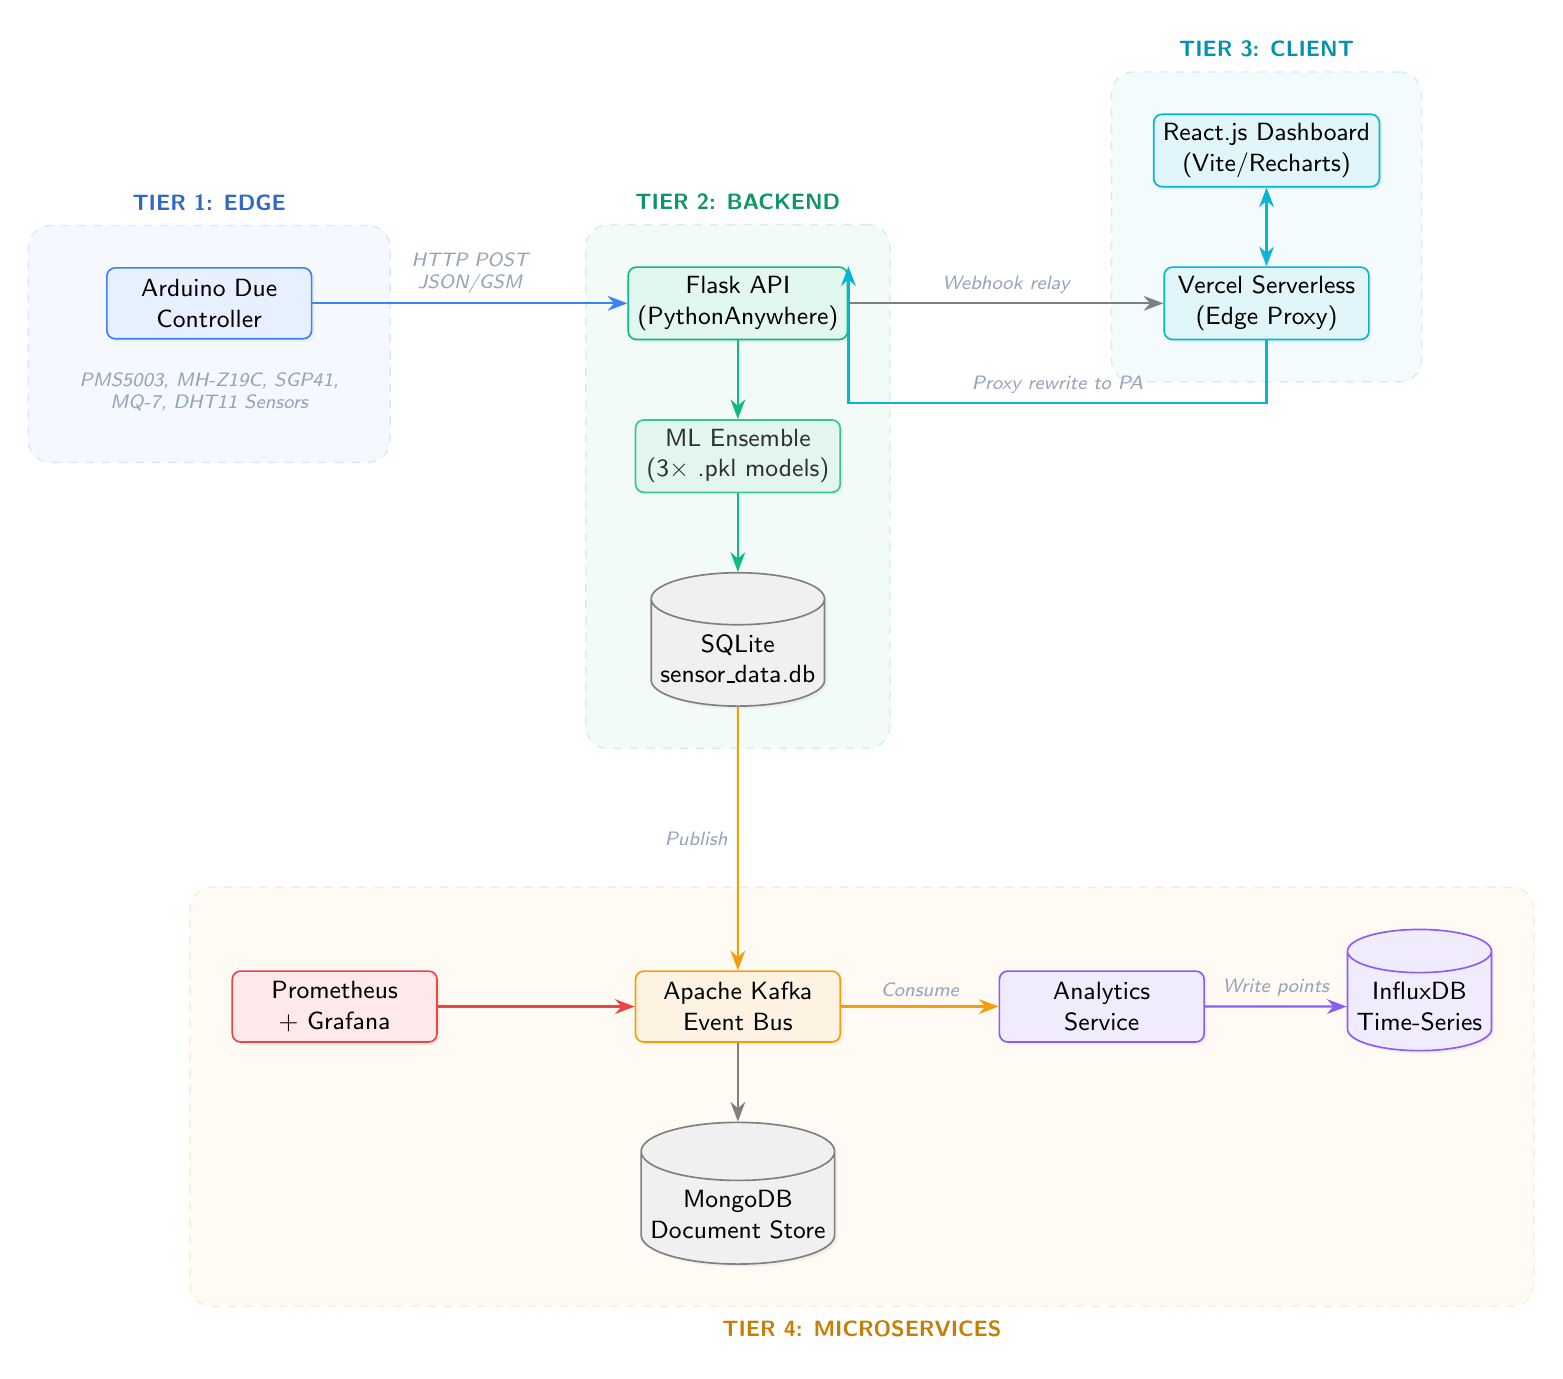
\begin{tikzpicture}[node distance=1.5cm and 2.5cm]

\node[sysblock=edgeblue] (arduino) {Arduino Due\\Controller};
\node[below=0.3cm of arduino, sysannot] (sensors) {PMS5003, MH-Z19C, SGP41,\\MQ-7, DHT11 Sensors};

\node[sysblock=flaskgreen, right=4cm of arduino] (flask) {Flask API\\(PythonAnywhere)};
\node[sysblock=flaskgreen, below=1cm of flask, opacity=0.8] (ml) {ML Ensemble\\(3$\times$ .pkl models)};
\node[sysdb=gray, below=1cm of ml] (sqlite) {SQLite\\sensor\_data.db};

\node[sysblock=reactcyan, right=4cm of flask] (vercel) {Vercel Serverless\\(Edge Proxy)};
\node[sysblock=reactcyan, above=1cm of vercel] (react) {React.js Dashboard\\(Vite/Recharts)};

\node[sysblock=kafkaorange, below=8cm of flask] (kafka) {Apache Kafka\\Event Bus};
\node[sysblock=influxpurple, right=2cm of kafka] (analytics) {Analytics\\Service};
\node[sysdb=influxpurple, right=1.8cm of analytics] (influx) {InfluxDB\\Time-Series};
\node[sysdb=gray, below=1cm of kafka] (mongo) {MongoDB\\Document Store};
\node[sysblock=dangered, left=2.5cm of kafka] (prom) {Prometheus\\+ Grafana};

\draw[sysarrow, edgeblue] (arduino) -- node[above, sysannot] {HTTP POST\\JSON/GSM} (flask);
\draw[sysarrow, flaskgreen] (flask) -- (ml);
\draw[sysarrow, flaskgreen] (ml) -- (sqlite);
\draw[sysarrow, gray] (flask) -- node[above, sysannot] {Webhook relay} (vercel);
\draw[sysdarrow, reactcyan] (vercel) -- (react);
\draw[sysarrow, reactcyan] (vercel.south) -- ++(0,-0.8) -| node[near start, above, sysannot] {Proxy rewrite to PA} (flask.north east);
\draw[sysarrow, kafkaorange] (sqlite.south) -- node[left, sysannot] {Publish} (kafka.north);
\draw[sysarrow, kafkaorange] (kafka) -- node[above, sysannot] {Consume} (analytics);
\draw[sysarrow, influxpurple] (analytics) -- node[above, sysannot] {Write points} (influx);
\draw[sysarrow, gray] (kafka) -- (mongo);
\draw[sysarrow, dangered] (prom) -- (kafka);

\begin{scope}[on background layer]
    \node[syscontainer=edgeblue, fit=(arduino) (sensors), label={[systier=edgeblue]above:TIER 1: EDGE}] {};
    \node[syscontainer=flaskgreen, fit=(flask) (ml) (sqlite), label={[systier=flaskgreen]above:TIER 2: BACKEND}] {};
    \node[syscontainer=reactcyan, fit=(vercel) (react), label={[systier=reactcyan]above:TIER 3: CLIENT}] {};
    \node[syscontainer=kafkaorange, fit=(kafka) (analytics) (influx) (mongo) (prom), label={[systier=kafkaorange]below:TIER 4: MICROSERVICES}] {};
\end{scope}

\end{tikzpicture}%
}
\caption{Complete AQMRG platform architecture showing the multi-tier data flow. Tiers are logically grouped by role, spanning from edge sensing to cloud-hosted analytics and event streaming via Apache Kafka.}
\label{fig:arch}
\end{figure}
}

\newcommand{\figMethodologyLifecycle}{%
\begin{figure}[H]
\centering
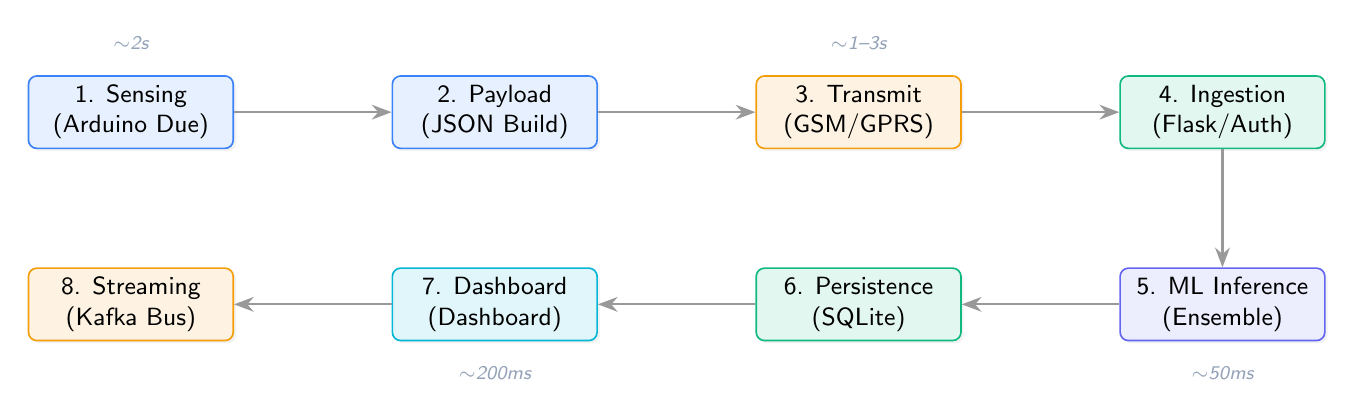
\begin{tikzpicture}[node distance=1cm and 2cm]

\node[sysblock=edgeblue] (p1) {1. Sensing\\(Arduino Due)};
\node[sysblock=edgeblue, right=of p1] (p2) {2. Payload\\(JSON Build)};
\node[sysblock=amber, right=of p2] (p3) {3. Transmit\\(GSM/GPRS)};
\node[sysblock=flaskgreen, right=of p3] (p4) {4. Ingestion\\(Flask/Auth)};

\node[sysblock=indigo, below=1.5cm of p4] (p5) {5. ML Inference\\(Ensemble)};
\node[sysblock=flaskgreen, left=of p5] (p6) {6. Persistence\\(SQLite)};
\node[sysblock=reactcyan, left=of p6] (p7) {7. Dashboard\\(Dashboard)};
\node[sysblock=kafkaorange, left=of p7] (p8) {8. Streaming\\(Kafka Bus)};

\draw[sysarrow] (p1) -- (p2);
\draw[sysarrow] (p2) -- (p3);
\draw[sysarrow] (p3) -- (p4);
\draw[sysarrow] (p4) -- (p5);
\draw[sysarrow] (p5) -- (p6);
\draw[sysarrow] (p6) -- (p7);
\draw[sysarrow] (p7) -- (p8);

\node[sysannot, above=0.2cm of p1] {$\sim$2s};
\node[sysannot, above=0.2cm of p3] {$\sim$1--3s};
\node[sysannot, below=0.2cm of p5] {$\sim$50ms};
\node[sysannot, below=0.2cm of p7] {$\sim$200ms};

\end{tikzpicture}
\caption{End-to-end data lifecycle in a compact snaking layout. Timing annotations indicate typical systemic latency from physical sensing to global dashboard availability.}
\label{fig:lifecycle}
\end{figure}
}

\newcommand{\figMethodologyDeploy}{%
\begin{figure}[H]
\centering
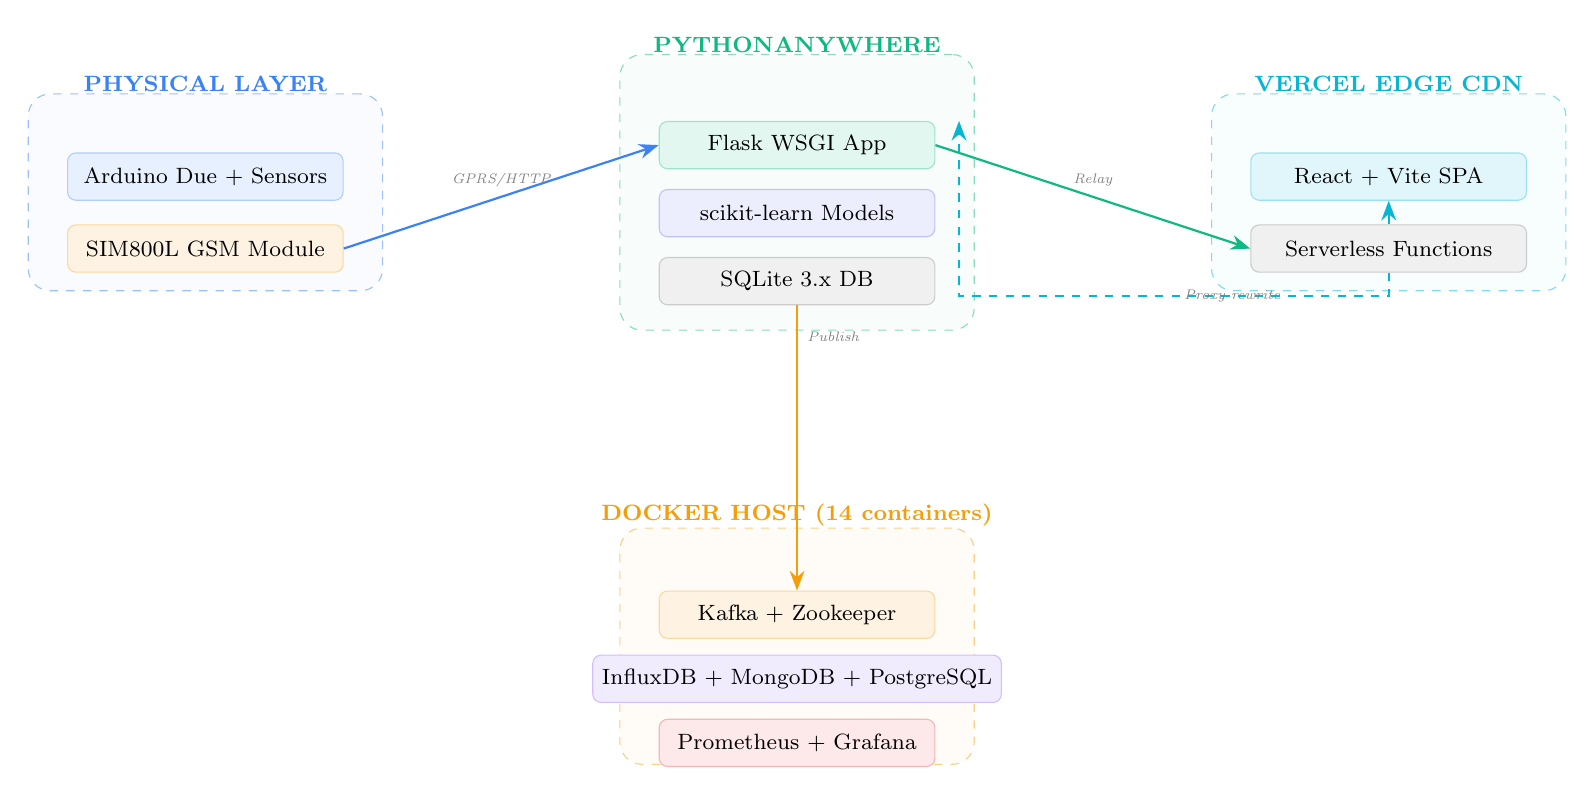
\begin{tikzpicture}[
    every node/.style={font=\small},
    cloudbox/.style={rectangle, draw, rounded corners=8pt, minimum width=4.5cm, minimum height=2cm, align=center, dashed, draw=#1!50, fill=#1!3},
    innerblock/.style={rectangle, draw, rounded corners=3pt, minimum width=3.5cm, minimum height=0.6cm, align=center, font=\footnotesize, fill=#1!12, draw=#1!40},
    arrow/.style={-{Stealth[length=2.5mm]}, thick}
]

\node[cloudbox=edgeblue, minimum height=2.5cm] (physical) at (0,0) {};
\node[above=-0.1cm of physical.north, font=\footnotesize\bfseries, text=edgeblue] {PHYSICAL LAYER};
\node[innerblock=edgeblue] (ard) at (0, 0.2) {Arduino Due + Sensors};
\node[innerblock=amber, below=0.3cm of ard] (gsm) {SIM800L GSM Module};

\node[cloudbox=flaskgreen, minimum height=3.5cm, right=3cm of physical] (pacloud) {};
\node[above=-0.1cm of pacloud.north, font=\footnotesize\bfseries, text=flaskgreen] {PYTHONANYWHERE};
\node[innerblock=flaskgreen] (flaskd) at ([yshift=0.6cm]pacloud.center) {Flask WSGI App};
\node[innerblock=indigo, below=0.25cm of flaskd] (mld) {scikit-learn Models};
\node[innerblock=gray, below=0.25cm of mld] (sqld) {SQLite 3.x DB};

\node[cloudbox=reactcyan, minimum height=2.5cm, right=3cm of pacloud] (vercelcloud) {};
\node[above=-0.1cm of vercelcloud.north, font=\footnotesize\bfseries, text=reactcyan] {VERCEL EDGE CDN};
\node[innerblock=reactcyan] (reactd) at ([yshift=0.2cm]vercelcloud.center) {React + Vite SPA};
\node[innerblock=gray, below=0.3cm of reactd] (sless) {Serverless Functions};

\node[cloudbox=kafkaorange, minimum height=3cm, below=2.5cm of pacloud] (docker) {};
\node[above=-0.1cm of docker.north, font=\footnotesize\bfseries, text=kafkaorange] {DOCKER HOST (14 containers)};
\node[innerblock=kafkaorange] (kd) at ([yshift=0.4cm]docker.center) {Kafka + Zookeeper};
\node[innerblock=influxpurple, below=0.2cm of kd] (idb) {InfluxDB + MongoDB + PostgreSQL};
\node[innerblock=dangered, below=0.2cm of idb] (obd) {Prometheus + Grafana};

\draw[arrow, edgeblue] (gsm.east) -- node[above, font=\tiny\itshape, text=gray] {GPRS/HTTP} (flaskd.west);
\draw[arrow, flaskgreen] (flaskd.east) -- node[above, font=\tiny\itshape, text=gray] {Relay} (sless.west);
\draw[arrow, reactcyan] (sless) -- (reactd);
\draw[arrow, kafkaorange] (sqld.south) -- ++(0,-0.4) -| node[near start, right, font=\tiny\itshape, text=gray] {Publish} (kd.north);
\draw[arrow, reactcyan, dashed] (sless.south) -- ++(0,-0.3) -| node[near start, right, font=\tiny\itshape, text=gray] {Proxy rewrite} ([xshift=0.3cm]flaskd.north east);

\end{tikzpicture}
\caption{Physical deployment topology showing the four hosting environments: a field-deployed Arduino node, PythonAnywhere's managed Python hosting, Vercel's edge CDN, and a Docker Compose cluster for microservices.}
\label{fig:deploy}
\end{figure}
}

\newcommand{\figMethodologyWiring}{%
\begin{figure}[H]
\centering
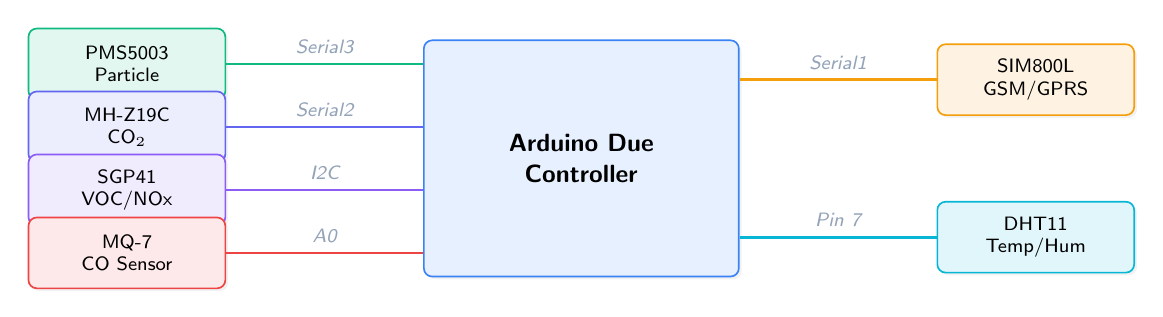
\begin{tikzpicture}[
    node distance=1cm and 2.5cm,
    sensor/.style={sysblock=#1, minimum width=2.5cm, font=\sffamily\scriptsize},
    bus/.style={draw=#1, thick, line width=1pt}
]

\node[sysblock=edgeblue, minimum width=4cm, minimum height=3cm] (mcu) {\textbf{Arduino Due}\\\textbf{Controller}};

\node[sensor=flaskgreen, left=of mcu, yshift=1.2cm] (pms) {PMS5003\\Particle};
\node[sensor=indigo, left=of mcu, yshift=0.4cm] (mhz) {MH-Z19C\\CO$_2$};
\node[sensor=influxpurple, left=of mcu, yshift=-0.4cm] (sgp) {SGP41\\VOC/NOx};
\node[sensor=dangered, left=of mcu, yshift=-1.2cm] (mq7) {MQ-7\\CO Sensor};

\node[sensor=amber, right=of mcu, yshift=1cm] (gsm) {SIM800L\\GSM/GPRS};
\node[sensor=reactcyan, right=of mcu, yshift=-1cm] (dht) {DHT11\\Temp/Hum};

\draw[bus=flaskgreen] (pms.east) -- node[above, sysannot] {Serial3} (mcu.west |- pms.east);
\draw[bus=indigo] (mhz.east) -- node[above, sysannot] {Serial2} (mcu.west |- mhz.east);
\draw[bus=influxpurple] (sgp.east) -- node[above, sysannot] {I2C} (mcu.west |- sgp.east);
\draw[bus=dangered] (mq7.east) -- node[above, sysannot] {A0} (mcu.west |- mq7.east);
\draw[bus=amber] (gsm.west) -- node[above, sysannot] {Serial1} (mcu.east |- gsm.west);
\draw[bus=reactcyan] (dht.west) -- node[above, sysannot] {Pin 7} (mcu.east |- dht.west);

\end{tikzpicture}
\caption{Hardware wiring topology. Sensor modules connect to the Arduino Due via diverse interfaces (UART, I2C, Analog, Digital), with the SIM800L module providing cellular connectivity.}
\label{fig:wiring}
\end{figure}
}

\newcommand{\figMethodologyPayload}{%
\begin{figure}[H]
\centering
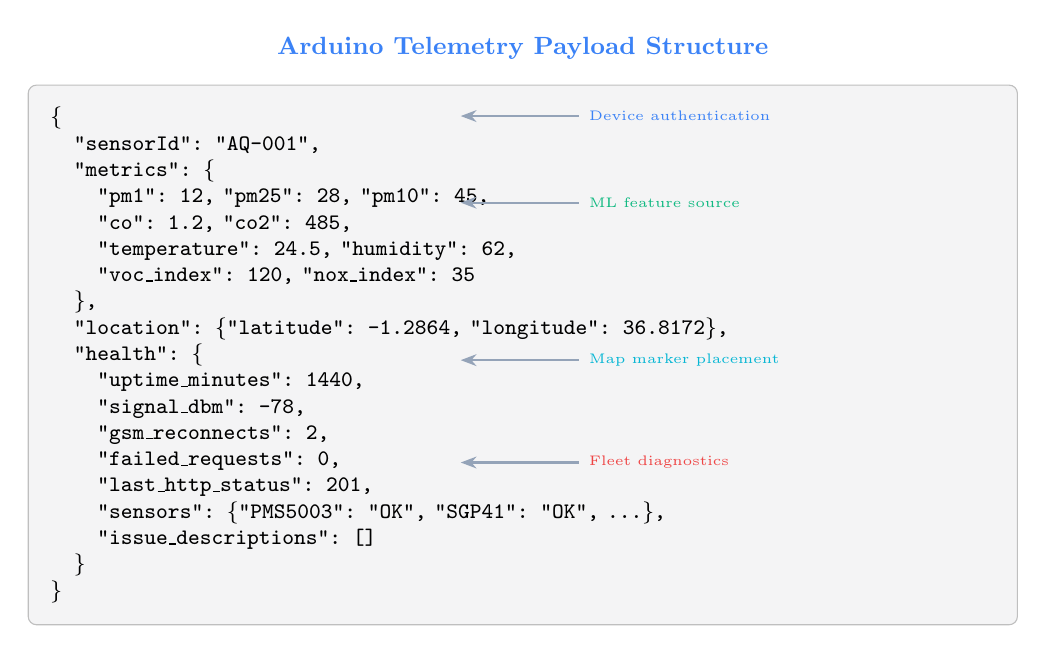
\begin{tikzpicture}[
    every node/.style={font=\footnotesize},
    jsonblock/.style={rectangle, draw=gray!50, fill=darkslate!5, rounded corners=3pt, minimum width=5cm, align=left, inner sep=8pt}
]

\node[jsonblock, text width=12cm] (json) {
\texttt{\{}\\
\quad\texttt{"sensorId": "AQ-001",}\\
\quad\texttt{"metrics": \{}\\
\quad\quad\texttt{"pm1": 12, "pm25": 28, "pm10": 45,}\\
\quad\quad\texttt{"co": 1.2, "co2": 485,}\\
\quad\quad\texttt{"temperature": 24.5, "humidity": 62,}\\
\quad\quad\texttt{"voc\_index": 120, "nox\_index": 35}\\
\quad\texttt{\},}\\
\quad\texttt{"location": \{"latitude": -1.2864, "longitude": 36.8172\},}\\
\quad\texttt{"health": \{}\\
\quad\quad\texttt{"uptime\_minutes": 1440,}\\
\quad\quad\texttt{"signal\_dbm": -78,}\\
\quad\quad\texttt{"gsm\_reconnects": 2,}\\
\quad\quad\texttt{"failed\_requests": 0,}\\
\quad\quad\texttt{"last\_http\_status": 201,}\\
\quad\quad\texttt{"sensors": \{"PMS5003": "OK", "SGP41": "OK", ...\},}\\
\quad\quad\texttt{"issue\_descriptions": []}\\
\quad\texttt{\}}\\
\texttt{\}}
};

\node[above=0.2cm of json, font=\small\bfseries, text=edgeblue] {Arduino Telemetry Payload Structure};

\draw[{Stealth[length=2mm]}-, thick, softgray] ([xshift=5.5cm, yshift=-0.4cm]json.north west) -- ++(1.5,0) node[right, font=\tiny, text=edgeblue] {Device authentication};
\draw[{Stealth[length=2mm]}-, thick, softgray] ([xshift=5.5cm, yshift=-1.5cm]json.north west) -- ++(1.5,0) node[right, font=\tiny, text=flaskgreen] {ML feature source};
\draw[{Stealth[length=2mm]}-, thick, softgray] ([xshift=5.5cm, yshift=-3.5cm]json.north west) -- ++(1.5,0) node[right, font=\tiny, text=reactcyan] {Map marker placement};
\draw[{Stealth[length=2mm]}-, thick, softgray] ([xshift=5.5cm, yshift=-4.8cm]json.north west) -- ++(1.5,0) node[right, font=\tiny, text=dangered] {Fleet diagnostics};

\end{tikzpicture}
\caption{Structure of the JSON telemetry payload transmitted from the Arduino Due to the Flask backend. Annotations indicate which downstream subsystem consumes each section.}
\label{fig:payload}
\end{figure}
}

\newcommand{\figMethodologyFirmwareFsm}{%
\begin{figure}[H]
\centering
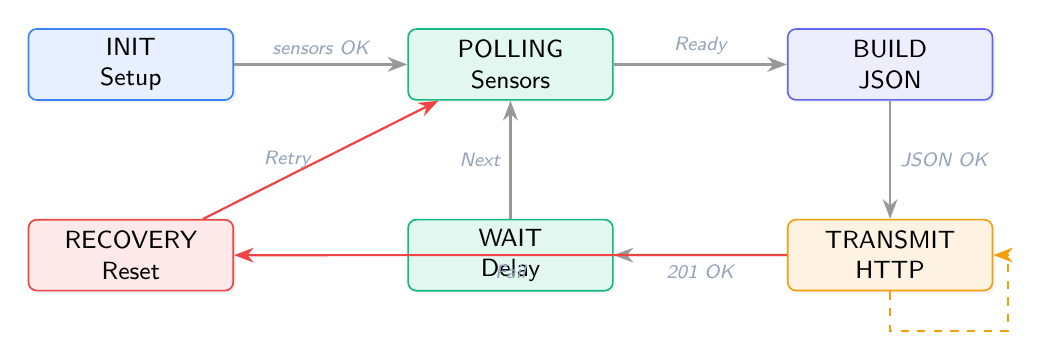
\begin{tikzpicture}[node distance=1.2cm and 2.2cm]

\node[sysblock=edgeblue] (init) {INIT\\Setup};
\node[sysblock=flaskgreen, right=of init] (sensor) {POLLING\\Sensors};
\node[sysblock=indigo, right=of sensor] (build) {BUILD\\JSON};
\node[sysblock=amber, below=1.5cm of build] (gsm) {TRANSMIT\\HTTP};
\node[sysblock=flaskgreen, below=1.5cm of sensor] (wait) {WAIT\\Delay};
\node[sysblock=dangered, below=1.5cm of init] (error) {RECOVERY\\Reset};

\draw[sysarrow] (init) -- node[above, sysannot] {sensors OK} (sensor);
\draw[sysarrow] (sensor) -- node[above, sysannot] {Ready} (build);
\draw[sysarrow] (build) -- node[right, sysannot] {JSON OK} (gsm);
\draw[sysarrow] (gsm) -- node[below, sysannot] {201 OK} (wait);
\draw[sysarrow] (wait) -- node[left, sysannot] {Next} (sensor);
\draw[sysarrow, dangered] (gsm.west) -- node[below, sysannot] {Fail} (error);
\draw[sysarrow, dangered] (error) -- node[left, sysannot] {Retry} (sensor);

\draw[sysarrow, dashed, amber] (gsm.south) -- ++(0,-0.5) -- ++(1.5,0) |- (gsm.east);

\end{tikzpicture}
\caption{Firmware state machine governing the operational lifecycle of the edge node, including polling cycles and fault recovery logic.}
\label{fig:firmware_fsm}
\end{figure}
}

\newcommand{\figMethodologyAppFactory}{%
\begin{figure}[H]
\centering
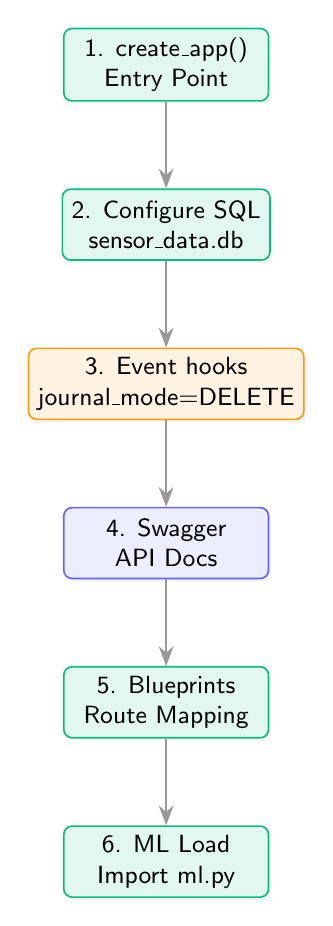
\begin{tikzpicture}[node distance=1.1cm]

\node[sysblock=flaskgreen] (s1) {1. create\_app()\\Entry Point};
\node[sysblock=flaskgreen, below=of s1] (s2) {2. Configure SQL\\sensor\_data.db};
\node[sysblock=amber, below=of s2] (s3) {3. Event hooks\\journal\_mode=DELETE};
\node[sysblock=indigo, below=of s3] (s4) {4. Swagger\\API Docs};
\node[sysblock=flaskgreen, below=of s4] (s5) {5. Blueprints\\Route Mapping};
\node[sysblock=emerald, below=of s5] (s6) {6. ML Load\\Import ml.py};

\draw[sysarrow] (s1) -- (s2);
\draw[sysarrow] (s2) -- (s3);
\draw[sysarrow] (s3) -- (s4);
\draw[sysarrow] (s4) -- (s5);
\draw[sysarrow] (s5) -- (s6);

\end{tikzpicture}
\caption{Flask application factory initialization flow. The system utilizes a singleton pattern for ML model loading during the WSGI server startup phase.}
\label{fig:app_factory}
\end{figure}
}

\newcommand{\figMethodologyErd}{%
\begin{figure}[H]
\centering
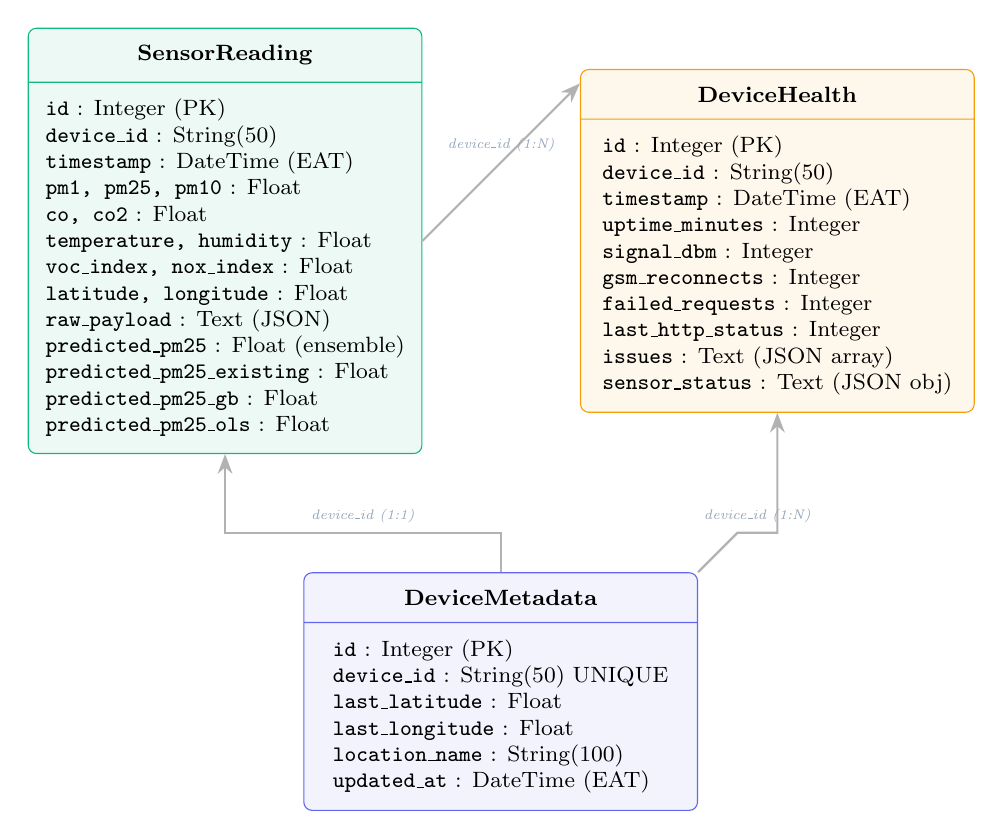
\begin{tikzpicture}[
    every node/.style={font=\small},
    entity/.style={rectangle split, rectangle split parts=2, draw=#1, fill=#1!8, rounded corners=3pt, minimum width=5cm, align=left, font=\footnotesize, inner sep=6pt},
    arrow/.style={-{Stealth[length=2.5mm]}, thick, gray!60},
    rel/.style={font=\tiny\itshape, text=softgray}
]

\node[entity=flaskgreen] (sr) {
    \textbf{SensorReading}
    \nodepart{second}
    \texttt{id} : Integer (PK)\\
    \texttt{device\_id} : String(50)\\
    \texttt{timestamp} : DateTime (EAT)\\
    \texttt{pm1, pm25, pm10} : Float\\
    \texttt{co, co2} : Float\\
    \texttt{temperature, humidity} : Float\\
    \texttt{voc\_index, nox\_index} : Float\\
    \texttt{latitude, longitude} : Float\\
    \texttt{raw\_payload} : Text (JSON)\\
    \texttt{predicted\_pm25} : Float (ensemble)\\
    \texttt{predicted\_pm25\_existing} : Float\\
    \texttt{predicted\_pm25\_gb} : Float\\
    \texttt{predicted\_pm25\_ols} : Float
};

\node[entity=amber, right=2cm of sr] (dh) {
    \textbf{DeviceHealth}
    \nodepart{second}
    \texttt{id} : Integer (PK)\\
    \texttt{device\_id} : String(50)\\
    \texttt{timestamp} : DateTime (EAT)\\
    \texttt{uptime\_minutes} : Integer\\
    \texttt{signal\_dbm} : Integer\\
    \texttt{gsm\_reconnects} : Integer\\
    \texttt{failed\_requests} : Integer\\
    \texttt{last\_http\_status} : Integer\\
    \texttt{issues} : Text (JSON array)\\
    \texttt{sensor\_status} : Text (JSON obj)
};

\node[entity=indigo, below=1.5cm of sr, xshift=3.5cm] (dm) {
    \textbf{DeviceMetadata}
    \nodepart{second}
    \texttt{id} : Integer (PK)\\
    \texttt{device\_id} : String(50) UNIQUE\\
    \texttt{last\_latitude} : Float\\
    \texttt{last\_longitude} : Float\\
    \texttt{location\_name} : String(100)\\
    \texttt{updated\_at} : DateTime (EAT)
};

\draw[arrow] (sr.east) -- node[above, rel] {device\_id (1:N)} ([yshift=2cm]dh.west);
\draw[arrow] (dm.north) -- ++(0,0.5) -| node[near start, above, rel] {device\_id (1:1)} (sr.south);
\draw[arrow] (dm.north east) -- ++(0.5,0.5) -| node[near start, above, rel] {device\_id (1:N)} (dh.south);

\end{tikzpicture}
\caption{Entity-Relationship diagram for the SQLite database. Each \texttt{SensorReading} stores raw sensor data plus all four prediction columns. \texttt{DeviceHealth} provides per-submission hardware diagnostics, and \texttt{DeviceMetadata} maintains persistent geographic identity per device.}
\label{fig:erd}
\end{figure}
}

\newcommand{\figMethodologyIngest}{%
\begin{figure}[H]
\centering
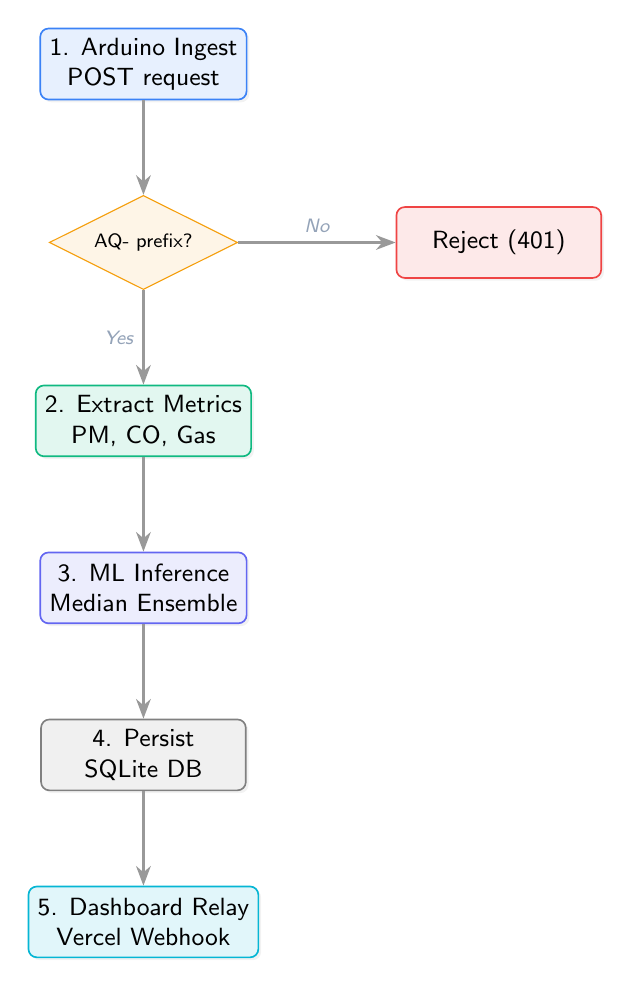
\begin{tikzpicture}[node distance=1.2cm]

\node[sysblock=edgeblue] (s1) {1. Arduino Ingest\\POST request};
\node[diamond, draw=amber, fill=amber!10, below=of s1, aspect=2, align=center, font=\sffamily\scriptsize] (d1) {AQ- prefix?};
\node[sysblock=dangered, right=2cm of d1] (reject) {Reject (401)};
\node[sysblock=flaskgreen, below=of d1] (s2) {2. Extract Metrics\\PM, CO, Gas};
\node[sysblock=indigo, below=of s2] (s3) {3. ML Inference\\Median Ensemble};
\node[sysblock=gray, below=of s3] (s4) {4. Persist\\SQLite DB};
\node[sysblock=reactcyan, below=of s4] (s5) {5. Dashboard Relay\\Vercel Webhook};

\draw[sysarrow] (s1) -- (d1);
\draw[sysarrow] (d1) -- node[above, sysannot] {No} (reject);
\draw[sysarrow] (d1) -- node[left, sysannot] {Yes} (s2);
\draw[sysarrow] (s2) -- (s3);
\draw[sysarrow] (s3) -- (s4);
\draw[sysarrow] (s4) -- (s5);

\end{tikzpicture}
\caption{Ingestion pipeline logic flow. Each request is validated, passed through the ML ensemble, and asynchronously relayed to the live dashboard within the HTTP cycle.}
\label{fig:ingest}
\end{figure}
}

\newcommand{\figMethodologyTrainingPipeline}{%
\begin{figure}[H]
\centering
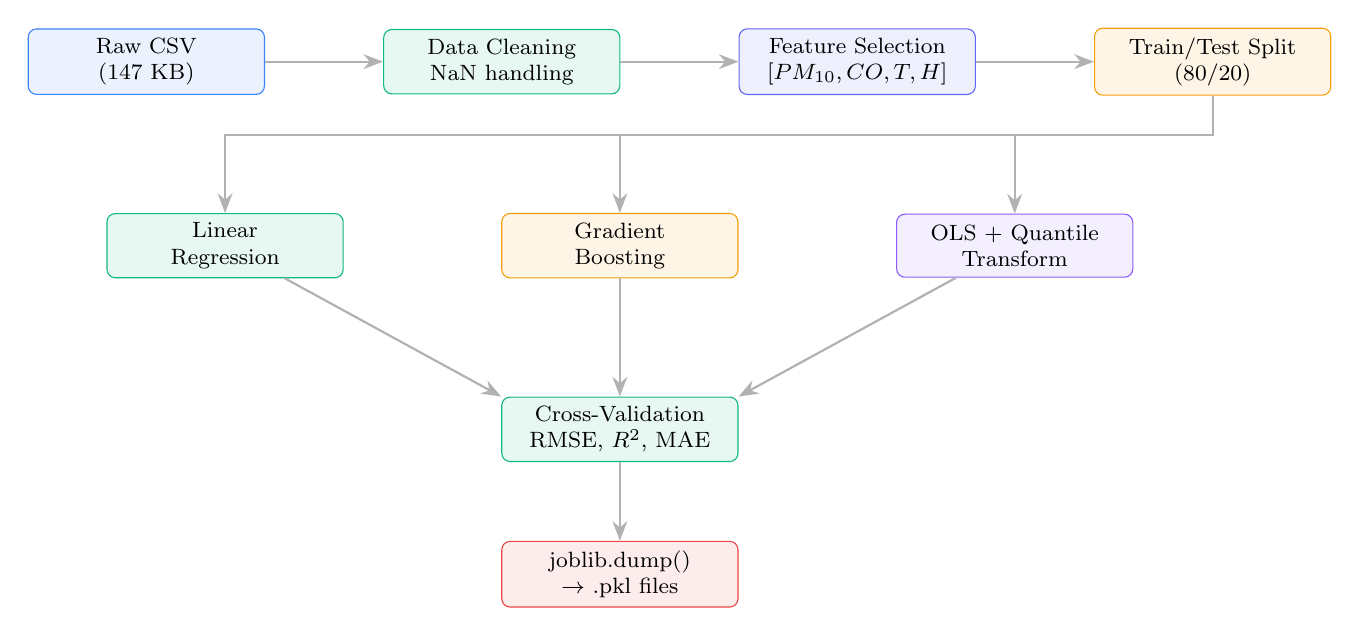
\begin{tikzpicture}[
    every node/.style={font=\small},
    block/.style={rectangle, draw=#1, fill=#1!10, rounded corners=3pt, minimum width=3cm, minimum height=0.8cm, align=center, font=\footnotesize},
    arrow/.style={-{Stealth[length=2.5mm]}, thick, gray!60}
]

\node[block=edgeblue] (raw) {Raw CSV\\(147 KB)};
\node[block=flaskgreen, right=1.5cm of raw] (clean) {Data Cleaning\\NaN handling};
\node[block=indigo, right=1.5cm of clean] (feat) {Feature Selection\\$[PM_{10}, CO, T, H]$};
\node[block=amber, right=1.5cm of feat] (split) {Train/Test Split\\(80/20)};

\node[block=flaskgreen, below=1.5cm of raw, xshift=1cm] (lr) {Linear\\Regression};
\node[block=kafkaorange, right=2cm of lr] (gb) {Gradient\\Boosting};
\node[block=influxpurple, right=2cm of gb] (ols) {OLS + Quantile\\Transform};

\node[block=emerald, below=1.5cm of gb] (eval) {Cross-Validation\\RMSE, $R^2$, MAE};
\node[block=dangered, below=1cm of eval] (serial) {joblib.dump()\\$\rightarrow$ .pkl files};

\draw[arrow] (raw) -- (clean);
\draw[arrow] (clean) -- (feat);
\draw[arrow] (feat) -- (split);

\draw[arrow] (split.south) -- ++(0,-0.5) -| (lr.north);
\draw[arrow] (split.south) -- ++(0,-0.5) -| (gb.north);
\draw[arrow] (split.south) -- ++(0,-0.5) -| (ols.north);

\draw[arrow] (lr) -- (eval.north west);
\draw[arrow] (gb) -- (eval);
\draw[arrow] (ols) -- (eval.north east);
\draw[arrow] (eval) -- (serial);

\end{tikzpicture}
\caption{ML training pipeline: raw CSV data undergoes cleaning and feature selection before being split into training/test sets. Three distinct algorithms are trained, cross-validated, and serialized for production deployment.}
\label{fig:training_pipeline}
\end{figure}
}

\newcommand{\figMethodologyMlpipeline}{%
\begin{figure}[H]
\centering
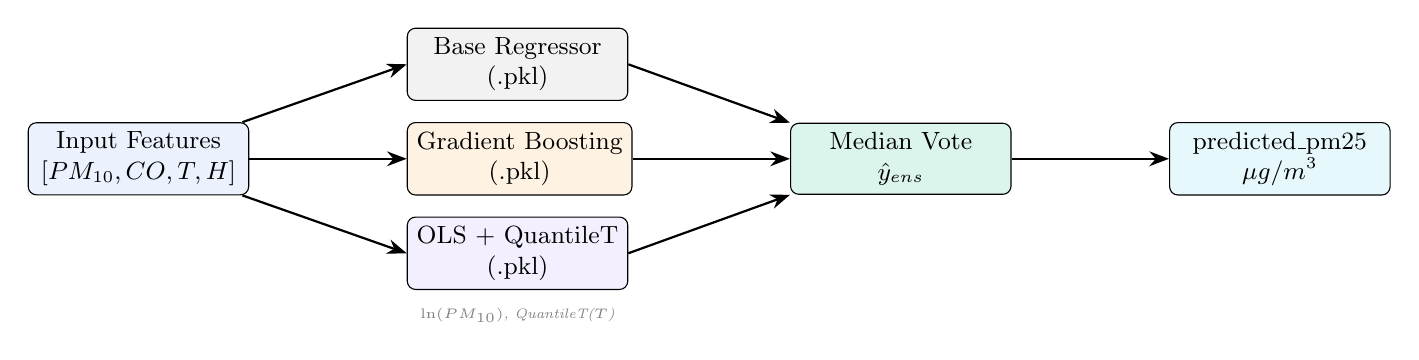
\begin{tikzpicture}[
    node distance=0.6cm and 1.5cm,
    every node/.style={font=\small},
    block/.style={rectangle, draw, rounded corners=3pt, minimum width=2.8cm, minimum height=0.8cm, align=center},
    arrow/.style={-{Stealth[length=2.5mm]}, thick}
]

\node[block, fill=edgeblue!10] (input) {Input Features\\$[PM_{10}, CO, T, H]$};

\node[block, fill=gray!10, right=2cm of input, yshift=1.2cm] (m1) {Base Regressor\\(.pkl)};
\node[block, fill=kafkaorange!12, right=2cm of input] (m2) {Gradient Boosting\\(.pkl)};
\node[block, fill=influxpurple!10, right=2cm of input, yshift=-1.2cm] (m3) {OLS + QuantileT\\(.pkl)};

\node[block, fill=flaskgreen!15, right=2cm of m2] (median) {Median Vote\\$\hat{y}_{ens}$};

\node[block, fill=reactcyan!10, right=2cm of median] (out) {predicted\_pm25\\$\mu g/m^3$};

\draw[arrow] (input) -- (m1.west);
\draw[arrow] (input) -- (m2.west);
\draw[arrow] (input) -- (m3.west);
\draw[arrow] (m1.east) -- (median.north west);
\draw[arrow] (m2.east) -- (median.west);
\draw[arrow] (m3.east) -- (median.south west);
\draw[arrow] (median) -- (out);

\node[below=0.1cm of m3, font=\tiny\itshape, text=gray] {$\ln(PM_{10})$, QuantileT($T$)};

\end{tikzpicture}
\caption{ML ensemble inference pipeline. Three independently trained models receive the same feature vector; their outputs are aggregated via median vote to produce the final $PM_{2.5}$ prediction.}
\label{fig:mlpipeline}
\end{figure}
}

\newcommand{\figMethodologyEnsembleLogic}{%
\begin{figure}[H]
\centering
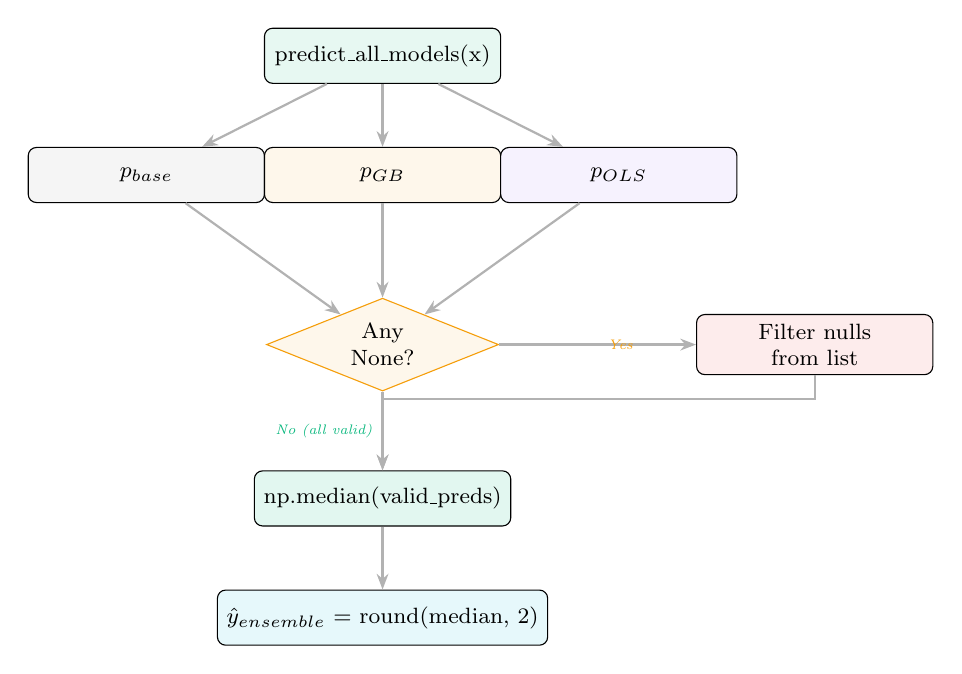
\begin{tikzpicture}[
    every node/.style={font=\small},
    block/.style={rectangle, draw, rounded corners=3pt, minimum width=3cm, minimum height=0.7cm, align=center, font=\footnotesize},
    decision/.style={diamond, draw=amber, fill=amber!8, minimum width=1.5cm, aspect=2.5, align=center, font=\footnotesize},
    arrow/.style={-{Stealth[length=2mm]}, thick, gray!60}
]

\node[block, fill=flaskgreen!10] (call) {predict\_all\_models(x)};
\node[block, fill=gray!8, below=0.8cm of call, xshift=-3cm] (p1) {$p_{base}$};
\node[block, fill=kafkaorange!8, below=0.8cm of call] (p2) {$p_{GB}$};
\node[block, fill=influxpurple!8, below=0.8cm of call, xshift=3cm] (p3) {$p_{OLS}$};

\node[decision, below=1.2cm of p2] (check) {Any\\None?};
\node[block, fill=dangered!10, right=2.5cm of check] (filter) {Filter nulls\\from list};

\node[block, fill=emerald!12, below=1cm of check] (median) {np.median(valid\_preds)};
\node[block, fill=reactcyan!10, below=0.8cm of median] (result) {$\hat{y}_{ensemble}$ = round(median, 2)};

\draw[arrow] (call) -- (p1);
\draw[arrow] (call) -- (p2);
\draw[arrow] (call) -- (p3);
\draw[arrow] (p1) -- (check);
\draw[arrow] (p2) -- (check);
\draw[arrow] (p3) -- (check);
\draw[arrow] (check) -- node[right, font=\tiny\itshape, text=amber] {Yes} (filter);
\draw[arrow] (filter.south) -- ++(0,-0.3) -| (median);
\draw[arrow] (check) -- node[left, font=\tiny\itshape, text=flaskgreen] {No (all valid)} (median);
\draw[arrow] (median) -- (result);

\end{tikzpicture}
\caption{Ensemble aggregation decision logic. Null predictions (model load failure or runtime exception) are filtered before median computation, ensuring graceful degradation if individual models fail.}
\label{fig:ensemble_logic}
\end{figure}
}

\newcommand{\figMethodologyComponentTree}{%
\begin{figure}[H]
\centering
\scalebox{0.9}{%
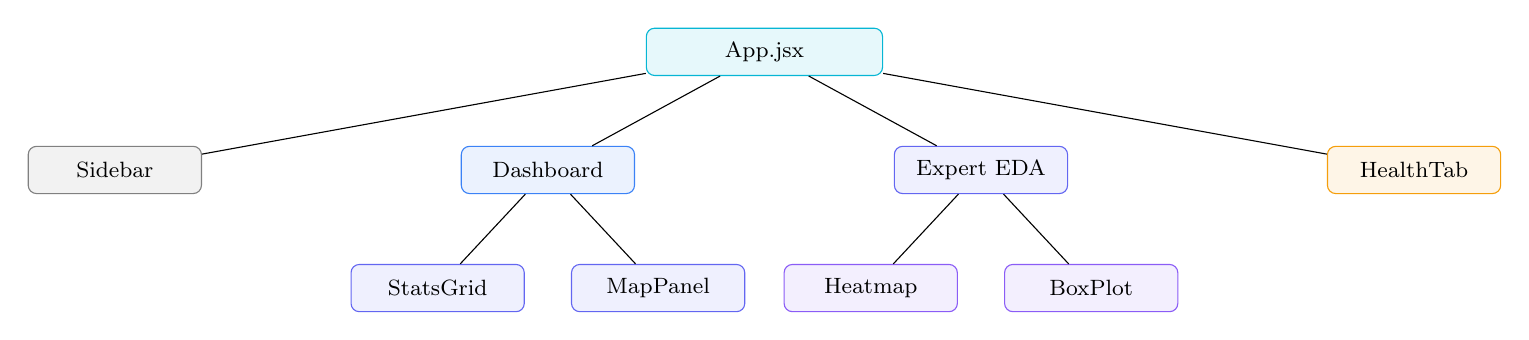
\begin{tikzpicture}[
    sysblock/.style={rectangle, draw=#1, fill=#1!10, rounded corners=3pt, minimum width=2.2cm, minimum height=0.6cm, align=center, font=\footnotesize},
    level 1/.style={sibling distance=5.5cm},
    level 2/.style={sibling distance=2.8cm, level distance=1.5cm},
    level 3/.style={sibling distance=1.8cm, level distance=1.5cm}
]

\node[sysblock=reactcyan, minimum width=3cm] (app) {App.jsx}
    child { node[sysblock=gray] {Sidebar} }
    child { node[sysblock=edgeblue] {Dashboard}
        child { node[sysblock=indigo] {StatsGrid} }
        child { node[sysblock=indigo] {MapPanel} }
    }
    child { node[sysblock=indigo] {Expert EDA}
        child { node[sysblock=influxpurple] {Heatmap} }
        child { node[sysblock=influxpurple] {BoxPlot} }
    }
    child { node[sysblock=amber] {HealthTab} };

\end{tikzpicture}%
}
\caption{Modular React.js component hierarchy. The architecture separates structural layout components from specialized visualization and diagnostic panels.}
\label{fig:component_tree}
\end{figure}
}

\newcommand{\figMethodologyPollFsm}{%
\begin{figure}[H]
\centering
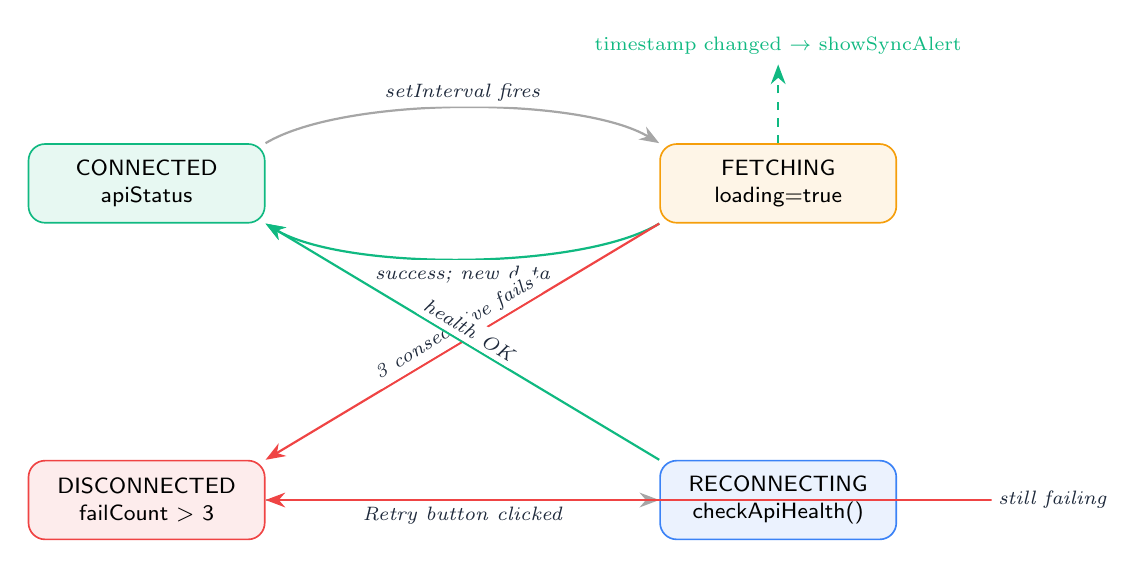
\begin{tikzpicture}[
    every node/.style={font=\small},
    state/.style={rectangle, draw=#1, fill=#1!10, rounded corners=6pt, minimum width=3cm, minimum height=1cm, align=center, font=\sffamily\footnotesize, line width=0.6pt},
    arrow/.style={-{Stealth[length=2.5mm]}, thick, gray!70, line width=0.8pt},
    annot/.style={font=\scriptsize\itshape, text=darkslate, fill=white, inner sep=2pt, rounded corners=1pt}
]

\node[state=flaskgreen] (conn) {CONNECTED\\apiStatus};
\node[state=amber, right=5cm of conn] (fetch) {FETCHING\\loading=true};
\node[state=dangered, below=3cm of conn] (disc) {DISCONNECTED\\failCount $>$ 3};
\node[state=edgeblue, below=3cm of fetch] (retry) {RECONNECTING\\checkApiHealth()};

% CONNECTED -> FETCHING (top, curved)
\draw[arrow] (conn.north east) .. controls +(1,0.6) and +(-1,0.6) .. node[above, annot] {setInterval fires} (fetch.north west);

% FETCHING -> CONNECTED (bottom, curved)
\draw[arrow, flaskgreen] (fetch.south west) .. controls +(-1,-0.6) and +(1,-0.6) .. node[below, annot] {success; new data} (conn.south east);

% FETCHING -> DISCONNECTED (diagonal)
\draw[arrow, dangered] (fetch.south west) -- node[annot, pos=0.5, sloped, above] {3 consecutive fails} (disc.north east);

% DISCONNECTED -> RECONNECTING
\draw[arrow] (disc) -- node[below, annot] {Retry button clicked} (retry);

% RECONNECTING -> CONNECTED
\draw[arrow, flaskgreen] (retry.north west) -- node[annot, pos=0.5, sloped, above] {health OK} (conn.south east);

% RECONNECTING -> DISCONNECTED (loop back)
\draw[arrow, dangered] (retry.east) -- ++(1.2,0) |- node[near start, annot, right] {still failing} (disc.east);

% Sync alert annotation
\draw[arrow, dashed, emerald] (fetch.north) -- ++(0,1) node[above, font=\scriptsize, text=emerald] {timestamp changed $\rightarrow$ showSyncAlert};

\end{tikzpicture}
\caption{Dashboard connection state machine. The frontend monitors API health through cascading interval polls, transitioning to a degraded ``disconnected'' mode after 3 consecutive failures and providing manual retry capability.}
\label{fig:poll_fsm}
\end{figure}
}

\newcommand{\figMethodologyIntelligenceMonitor}{%
\begin{figure}[H]
\centering
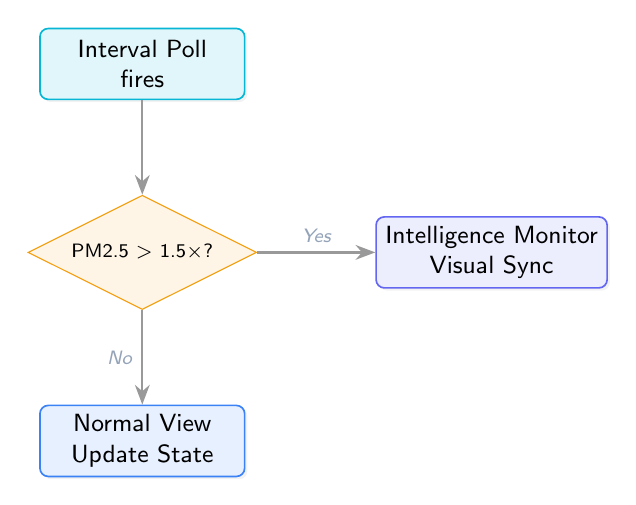
\begin{tikzpicture}[node distance=1.2cm]

\node[sysblock=reactcyan] (start) {Interval Poll\\fires};
\node[diamond, draw=amber, fill=amber!10, below=of start, aspect=2, align=center, font=\sffamily\scriptsize] (d1) {PM2.5 $>$ 1.5$\times$?};
\node[sysblock=indigo, right=1.5cm of d1] (alert) {Intelligence Monitor\\Visual Sync};
\node[sysblock=edgeblue, below=of d1] (pass) {Normal View\\Update State};

\draw[sysarrow] (start) -- (d1);
\draw[sysarrow] (d1) -- node[above, sysannot] {Yes} (alert);
\draw[sysarrow] (d1) -- node[left, sysannot] {No} (pass);

\end{tikzpicture}
\caption{Intelligence Monitor logic flow for real-time anomaly detection and visual state synchronisation.}
\label{fig:intelligence_monitor}
\end{figure}
}

\newcommand{\figMethodologyEdaFlow}{%
\begin{figure}[H]
\centering
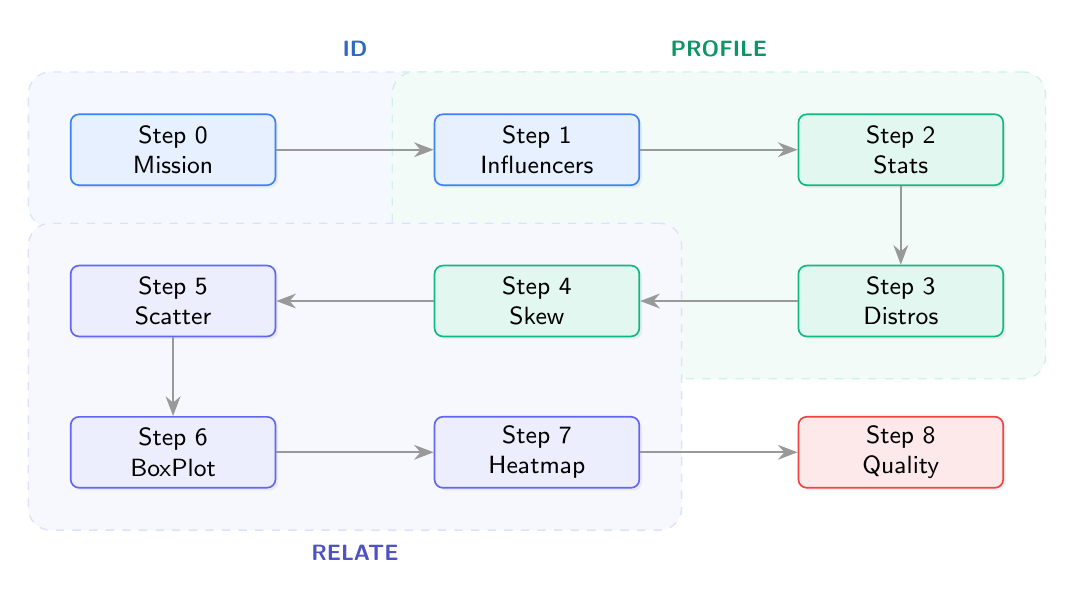
\begin{tikzpicture}[node distance=1cm and 2cm]

\node[sysblock=edgeblue] (s0) {Step 0\\Mission};
\node[sysblock=edgeblue, right=of s0] (s1) {Step 1\\Influencers};
\node[sysblock=flaskgreen, right=of s1] (s2) {Step 2\\Stats};

\node[sysblock=flaskgreen, below=of s2] (s3) {Step 3\\Distros};
\node[sysblock=flaskgreen, left=of s3] (s4) {Step 4\\Skew};
\node[sysblock=indigo, left=of s4] (s5) {Step 5\\Scatter};

\node[sysblock=indigo, below=of s5] (s6) {Step 6\\BoxPlot};
\node[sysblock=indigo, right=of s6] (s7) {Step 7\\Heatmap};
\node[sysblock=dangered, right=of s7] (s8) {Step 8\\Quality};

\draw[sysarrow] (s0) -- (s1);
\draw[sysarrow] (s1) -- (s2);
\draw[sysarrow] (s2) -- (s3);
\draw[sysarrow] (s3) -- (s4);
\draw[sysarrow] (s4) -- (s5);
\draw[sysarrow] (s5) -- (s6);
\draw[sysarrow] (s6) -- (s7);
\draw[sysarrow] (s7) -- (s8);

\begin{scope}[on background layer]
    \node[syscontainer=edgeblue, fit=(s0) (s1), label={[systier=edgeblue]above:ID}] {};
    \node[syscontainer=flaskgreen, fit=(s2) (s3) (s4), label={[systier=flaskgreen]above:PROFILE}] {};
    \node[syscontainer=indigo, fit=(s5) (s6) (s7), label={[systier=indigo]below:RELATE}] {};
\end{scope}

\end{tikzpicture}
\caption{The 9-step guided EDA workflow. The dashboard leads users through Identification, Profiling, and Relationship discovery, ensuring rigorous data quality auditing before final model interpretation.}
\label{fig:eda_flow}
\end{figure}
}

\newcommand{\figMethodologyMitigation}{%
\begin{figure}[H]
\centering
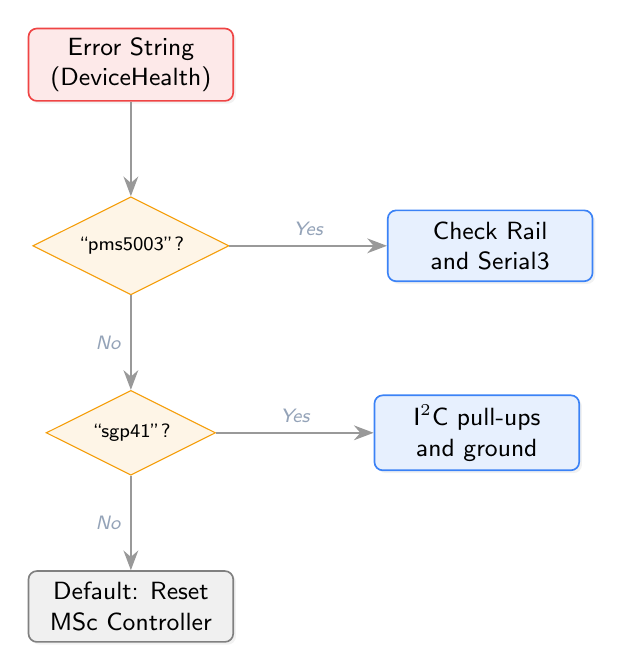
\begin{tikzpicture}[node distance=1.2cm]

\node[sysblock=dangered] (input) {Error String\\(DeviceHealth)};
\node[diamond, draw=amber, fill=amber!10, below=of input, aspect=2, align=center, font=\sffamily\scriptsize] (d1) {``pms5003''?};
\node[sysblock=edgeblue, right=2cm of d1] (a1) {Check Rail\\and Serial3};
\node[diamond, draw=amber, fill=amber!10, below=of d1, aspect=2, align=center, font=\sffamily\scriptsize] (d2) {``sgp41''?};
\node[sysblock=edgeblue, right=2cm of d2] (a2) {I$^2$C pull-ups\\and ground};
\node[sysblock=gray, below=of d2] (fallback) {Default: Reset\\MSc Controller};

\draw[sysarrow] (input) -- (d1);
\draw[sysarrow] (d1) -- node[above, sysannot] {Yes} (a1);
\draw[sysarrow] (d1) -- node[left, sysannot] {No} (d2);
\draw[sysarrow] (d2) -- node[above, sysannot] {Yes} (a2);
\draw[sysarrow] (d2) -- node[left, sysannot] {No} (fallback);

\end{tikzpicture}
\caption{Mitigation Engine decision tree. The system performs cascading string pattern matching on hardware diagnostic telemetry to generate actionable troubleshooting advice.}
\label{fig:mitigation}
\end{figure}
}

\newcommand{\figMethodologyDockerTopology}{%
\begin{figure}[H]
\centering
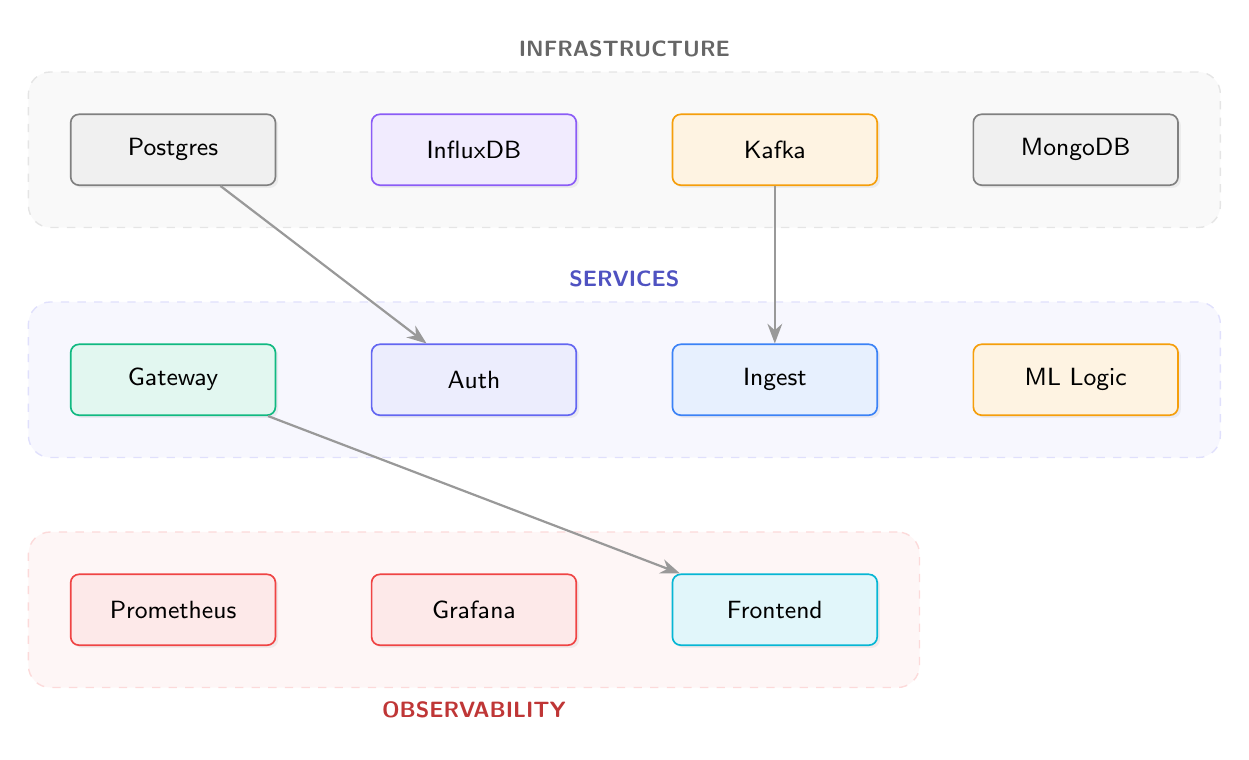
\begin{tikzpicture}[node distance=0.8cm and 1.2cm]

\node[sysblock=gray] (pg) {Postgres};
\node[sysblock=influxpurple, right=of pg] (influx) {InfluxDB};
\node[sysblock=kafkaorange, right=of influx] (kafka) {Kafka};
\node[sysblock=gray, right=of kafka] (mongo) {MongoDB};

\node[sysblock=flaskgreen, below=2cm of pg] (api) {Gateway};
\node[sysblock=indigo, right=of api] (auth) {Auth};
\node[sysblock=edgeblue, right=of auth] (ingest) {Ingest};
\node[sysblock=amber, right=of ingest] (ml) {ML Logic};

\node[sysblock=dangered, below=2cm of api] (prom) {Prometheus};
\node[sysblock=dangered, right=of prom] (graf) {Grafana};
\node[sysblock=reactcyan, right=of graf] (front) {Frontend};

\draw[sysarrow] (kafka) -- (ingest);
\draw[sysarrow] (pg) -- (auth);
\draw[sysarrow] (api) -- (front);

\begin{scope}[on background layer]
    \node[syscontainer=gray, fit=(pg) (influx) (kafka) (mongo), label={[systier=gray]above:INFRASTRUCTURE}] {};
    \node[syscontainer=indigo, fit=(api) (auth) (ingest) (ml), label={[systier=indigo]above:SERVICES}] {};
    \node[syscontainer=dangered, fit=(prom) (graf) (front), label={[systier=dangered]below:OBSERVABILITY}] {};
\end{scope}

\end{tikzpicture}
\caption{Containerized microservices topology. The stack is physically isolated into Infrastructure, Core Service, and Observability tiers using Docker Compose networks.}
\label{fig:docker_topology}
\end{figure}
}

\newcommand{\figMethodologyKafkaBridge}{%
\begin{figure}[H]
\centering
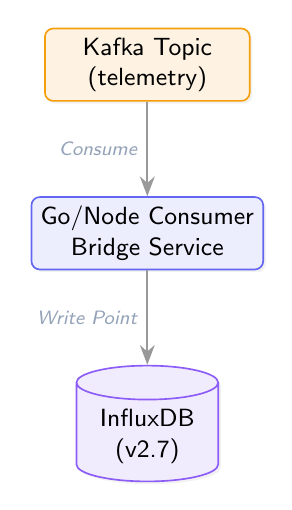
\begin{tikzpicture}[node distance=1.2cm]

\node[sysblock=kafkaorange] (k) {Kafka Topic\\(telemetry)};
\node[sysblock=indigo, below=of k] (c) {Go/Node Consumer\\Bridge Service};
\node[sysdb=influxpurple, below=of c] (i) {InfluxDB\\(v2.7)};

\draw[sysarrow] (k) -- node[left, sysannot] {Consume} (c);
\draw[sysarrow] (c) -- node[left, sysannot] {Write Point} (i);

\end{tikzpicture}
\caption{The Kafka-to-InfluxDB bridge flow for high-resolution time-series storage.}
\label{fig:kafka_bridge}
\end{figure}
}

\newcommand{\figMethodologySequence}{%
\begin{figure}[H]
\centering
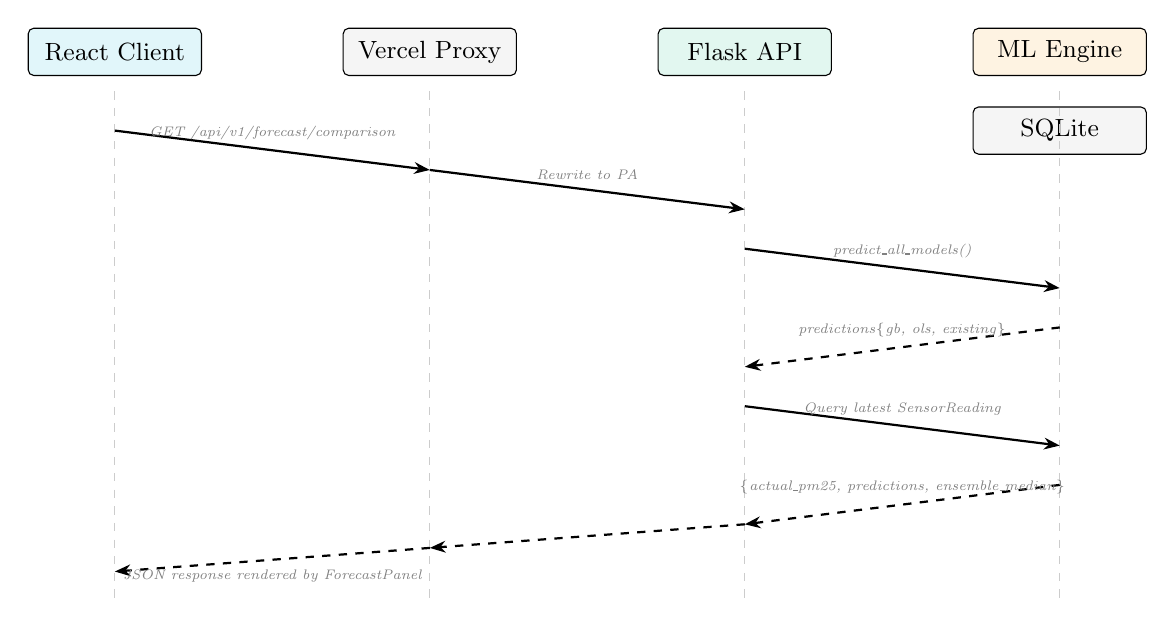
\begin{tikzpicture}[
    every node/.style={font=\small},
    actor/.style={rectangle, draw, rounded corners=2pt, minimum width=2.2cm, minimum height=0.6cm, align=center, fill=gray!5},
    arrow/.style={-{Stealth[length=2mm]}, thick},
    darrow/.style={{Stealth[length=2mm]}-{Stealth[length=2mm]}, thick},
    note/.style={font=\tiny\itshape, text=gray}
]

\node[actor, fill=reactcyan!12] (user) at (0,0) {React Client};
\node[actor, fill=gray!8] (vercel) at (4,0) {Vercel Proxy};
\node[actor, fill=flaskgreen!12] (flask) at (8,0) {Flask API};
\node[actor, fill=kafkaorange!12] (ml) at (12,0) {ML Engine};
\node[actor, fill=gray!8] (db) at (12,-1) {SQLite};

\draw[dashed, gray!40] (0,-0.5) -- (0,-7);
\draw[dashed, gray!40] (4,-0.5) -- (4,-7);
\draw[dashed, gray!40] (8,-0.5) -- (8,-7);
\draw[dashed, gray!40] (12,-0.5) -- (12,-7);

\draw[arrow] (0,-1) -- node[above, note] {GET /api/v1/forecast/comparison} (4,-1.5);
\draw[arrow] (4,-1.5) -- node[above, note] {Rewrite to PA} (8,-2);
\draw[arrow] (8,-2.5) -- node[above, note] {predict\_all\_models()} (12,-3);
\draw[arrow, dashed] (12,-3.5) -- node[above, note] {predictions\{gb, ols, existing\}} (8,-4);
\draw[arrow] (8,-4.5) -- node[above, note] {Query latest SensorReading} (12,-5);
\draw[arrow, dashed] (12,-5.5) -- node[above, note] {\{actual\_pm25, predictions, ensemble\_median\}} (8,-6);
\draw[arrow, dashed] (8,-6) -- (4,-6.3);
\draw[arrow, dashed] (4,-6.3) -- node[below, note] {JSON response rendered by ForecastPanel} (0,-6.6);

\end{tikzpicture}
\caption{Request-response sequence for ML forecast comparison.}
\label{fig:sequence}
\end{figure}
}

\newcommand{\figMethodologySeqIngest}{%
\begin{figure}[H]
\centering
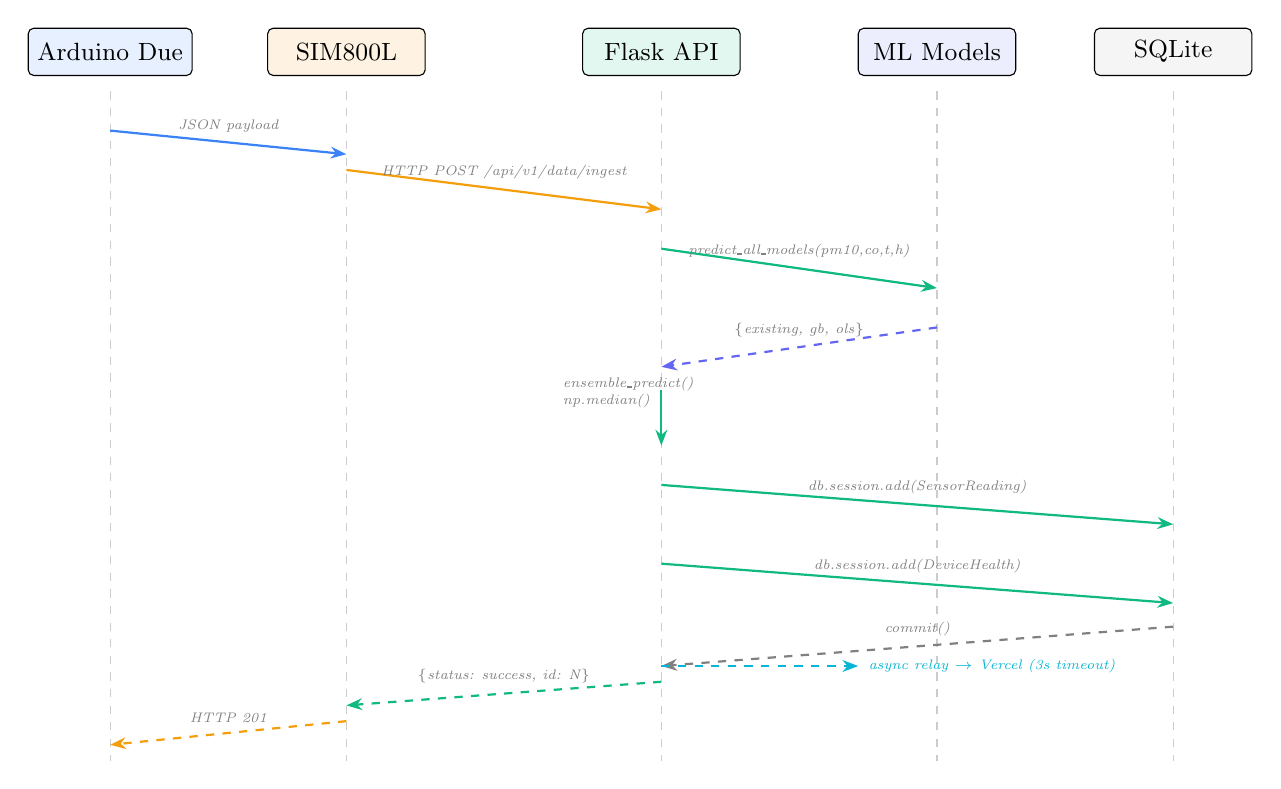
\begin{tikzpicture}[
    every node/.style={font=\small},
    actor/.style={rectangle, draw, rounded corners=2pt, minimum width=2cm, minimum height=0.6cm, align=center, fill=gray!5},
    arrow/.style={-{Stealth[length=2mm]}, thick},
    note/.style={font=\tiny\itshape, text=gray}
]

\node[actor, fill=edgeblue!12] (ard) at (0,0) {Arduino Due};
\node[actor, fill=amber!12] (gsm) at (3,0) {SIM800L};
\node[actor, fill=flaskgreen!12] (flask) at (7,0) {Flask API};
\node[actor, fill=indigo!12] (ml) at (10.5,0) {ML Models};
\node[actor, fill=gray!8] (db) at (13.5,0) {SQLite};

\foreach \x in {0,3,7,10.5,13.5} {
    \draw[dashed, gray!40] (\x,-0.5) -- (\x,-9);
}

\draw[arrow, edgeblue] (0,-1) -- node[above, note] {JSON payload} (3,-1.3);
\draw[arrow, amber] (3,-1.5) -- node[above, note] {HTTP POST /api/v1/data/ingest} (7,-2);
\draw[arrow, flaskgreen] (7,-2.5) -- node[above, note] {predict\_all\_models(pm10,co,t,h)} (10.5,-3);
\draw[arrow, dashed, indigo] (10.5,-3.5) -- node[above, note] {\{existing, gb, ols\}} (7,-4);
\draw[arrow, flaskgreen] (7,-4.3) -- node[above, note, text width=2.5cm] {ensemble\_predict()\\np.median()} (7,-5);
\draw[arrow, flaskgreen] (7,-5.5) -- node[above, note] {db.session.add(SensorReading)} (13.5,-6);
\draw[arrow, flaskgreen] (7,-6.5) -- node[above, note] {db.session.add(DeviceHealth)} (13.5,-7);
\draw[arrow, dashed, gray] (13.5,-7.3) -- node[above, note] {commit()} (7,-7.8);
\draw[arrow, dashed, flaskgreen] (7,-8) -- node[above, note] {\{status: success, id: N\}} (3,-8.3);
\draw[arrow, dashed, amber] (3,-8.5) -- node[above, note] {HTTP 201} (0,-8.8);

\draw[arrow, dashed, reactcyan] (7,-7.8) -- ++(2.5,0) node[right, note, text=reactcyan] {async relay $\rightarrow$ Vercel (3s timeout)};

\end{tikzpicture}
\caption{Arduino ingestion sequence diagram. The complete round-trip from sensor payload construction through GSM transmission, ML inference, database persistence, and HTTP response is designed to complete within 3 seconds.}
\label{fig:seq_ingest}
\end{figure}
}

\newcommand{\figMethodologyMonitoring}{%
\begin{figure}[H]
\centering
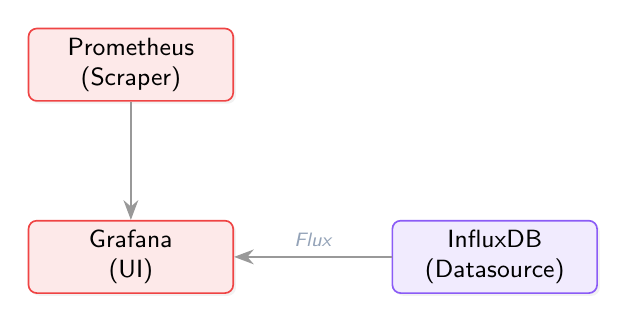
\begin{tikzpicture}[node distance=1.5cm]

\node[sysblock=dangered] (p) {Prometheus\\(Scraper)};
\node[sysblock=dangered, below=of p] (g) {Grafana\\(UI)};
\node[sysblock=influxpurple, right=2cm of g] (i) {InfluxDB\\(Datasource)};

\draw[sysarrow] (p) -- (g);
\draw[sysarrow] (i) -- node[above, sysannot] {Flux} (g);

\end{tikzpicture}
\caption{The Observability stack for real-time monitoring and historical analysis.}
\label{fig:monitoring}
\end{figure}
}

\newcommand{\figExpectedOutcomesR2Comparison}{%
\begin{figure}[H]
\centering
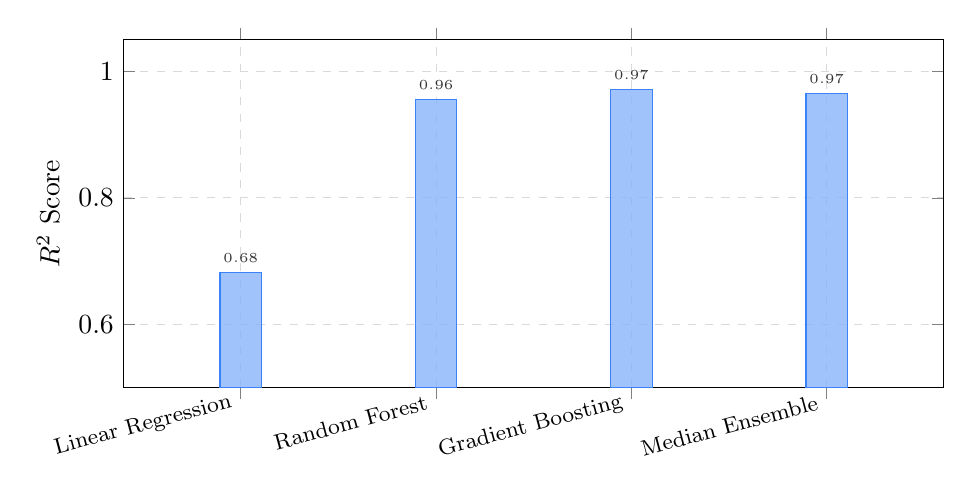
\begin{tikzpicture}
\begin{axis}[
    ybar,
    bar width=15pt,
    width=12cm,
    height=6cm,
    ylabel={$R^2$ Score},
    symbolic x coords={Linear Regression, Random Forest, Gradient Boosting, Median Ensemble},
    xtick=data,
    x tick label style={rotate=15, anchor=east, font=\footnotesize},
    ymin=0.5, ymax=1.05,
    enlarge x limits=0.2,
    nodes near coords,
    nodes near coords style={font=\tiny},
    every axis plot/.append style={fill opacity=0.8},
    grid=major,
    grid style={dashed, gray!30}
]
\addplot[fill=edgeblue!60, draw=edgeblue] coordinates {
    (Linear Regression, 0.682)
    (Random Forest, 0.9562)
    (Gradient Boosting, 0.9715)
    (Median Ensemble, 0.965)
};
\end{axis}
\end{tikzpicture}
\caption{Comparative $R^2$ scores across the four model approaches. Gradient Boosting achieves the highest individual score (0.9715), while the median ensemble provides variance-reduced production stability.}
\label{fig:r2_comparison}
\end{figure}
}

\newcommand{\figExpectedOutcomesRmseComparison}{%
\begin{figure}[H]
\centering
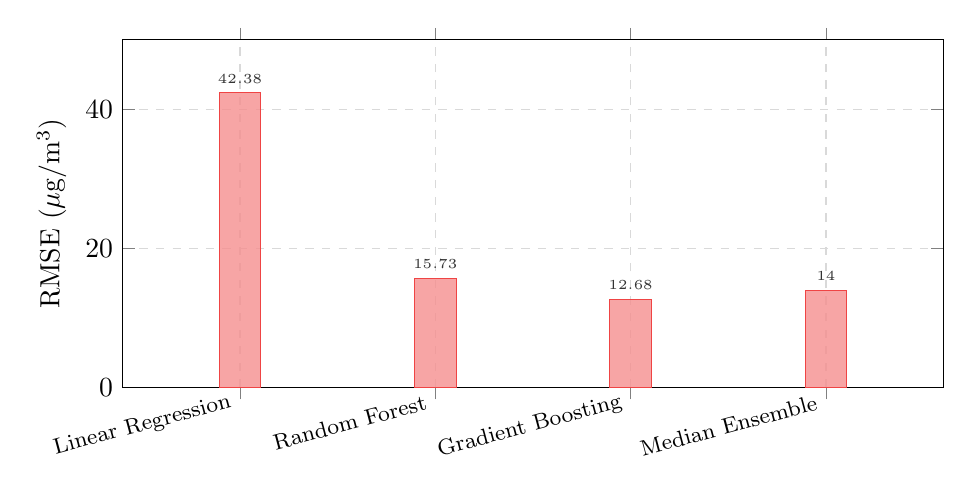
\begin{tikzpicture}
\begin{axis}[
    ybar,
    bar width=15pt,
    width=12cm,
    height=6cm,
    ylabel={RMSE ($\mu$g/m$^3$)},
    symbolic x coords={Linear Regression, Random Forest, Gradient Boosting, Median Ensemble},
    xtick=data,
    x tick label style={rotate=15, anchor=east, font=\footnotesize},
    ymin=0, ymax=50,
    enlarge x limits=0.2,
    nodes near coords,
    nodes near coords style={font=\tiny},
    every axis plot/.append style={fill opacity=0.8},
    grid=major,
    grid style={dashed, gray!30}
]
\addplot[fill=dangered!60, draw=dangered] coordinates {
    (Linear Regression, 42.38)
    (Random Forest, 15.73)
    (Gradient Boosting, 12.68)
    (Median Ensemble, 14.0)
};
\end{axis}
\end{tikzpicture}
\caption{RMSE comparison across models. The progression from Linear Regression (42.38) to Gradient Boosting (12.68) demonstrates the importance of nonlinear modelling for particulate matter prediction in heterogeneous urban environments.}
\label{fig:rmse_comparison}
\end{figure}
}

\newcommand{\figExpectedOutcomesRepo}{%
\begin{figure}[H]
\centering
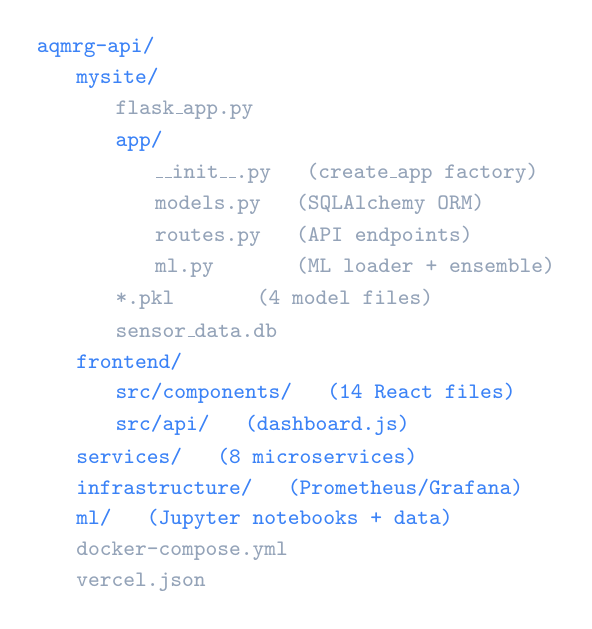
\begin{tikzpicture}[
    every node/.style={font=\footnotesize\ttfamily, anchor=west},
    dir/.style={text=edgeblue, font=\footnotesize\ttfamily\bfseries},
    file/.style={text=softgray}
]

\node[dir] at (0,0) {aqmrg-api/};
\node[dir] at (0.5,-0.4) {mysite/};
\node[file] at (1,-0.8) {flask\_app.py};
\node[dir] at (1,-1.2) {app/};
\node[file] at (1.5,-1.6) {\_\_init\_\_.py \ \ (create\_app factory)};
\node[file] at (1.5,-2.0) {models.py \ \ (SQLAlchemy ORM)};
\node[file] at (1.5,-2.4) {routes.py \ \ (API endpoints)};
\node[file] at (1.5,-2.8) {ml.py \ \ \ \ \ \ (ML loader + ensemble)};
\node[file] at (1,-3.2) {*.pkl \ \ \ \ \ \ (4 model files)};
\node[file] at (1,-3.6) {sensor\_data.db};
\node[dir] at (0.5,-4.0) {frontend/};
\node[dir] at (1,-4.4) {src/components/ \ \ (14 React files)};
\node[dir] at (1,-4.8) {src/api/ \ \ (dashboard.js)};
\node[dir] at (0.5,-5.2) {services/ \ \ (8 microservices)};
\node[dir] at (0.5,-5.6) {infrastructure/ \ \ (Prometheus/Grafana)};
\node[dir] at (0.5,-6.0) {ml/ \ \ (Jupyter notebooks + data)};
\node[file] at (0.5,-6.4) {docker-compose.yml};
\node[file] at (0.5,-6.8) {vercel.json};

\end{tikzpicture}
\caption{Simplified repository structure showing the key directories and files across all four platform tiers.}
\label{fig:repo}
\end{figure}
}

\newcommand{\figWorkplanBudgetGantt}{%
\begin{figure}[htbp]
  \centering
  \begin{ganttchart}[
      hgrid,
      vgrid={*{1}{draw=gray!30, dashed}},
      x unit         = 1.0cm,
      y unit title   = 0.65cm,
      y unit chart   = 0.6cm,
      title height   = 1,
      bar height     = 0.55,
      bar/.style={fill=RoyalBlue!70, rounded corners=2pt},
      title label font  = \small,
      bar label font    = \small,
  ]{1}{12}
    \gantttitle{Month, 2026--2027}{12}\\
    \gantttitlelist{1,...,12}{1}\\
    \ganttbar{Literature Review}{1}{2}\\
    \ganttbar{Sensor Procurement \& Setup}{1}{3}\\
    \ganttbar{Network Deployment}{3}{4}\\
    \ganttbar{Cloud Platform Development}{2}{5}\\
    \ganttbar{Data Collection}{5}{9}\\
    \ganttbar{AI Model Training}{5}{8}\\
    \ganttbar{Health Data Integration}{6}{9}\\
    \ganttbar{Analysis \& Mapping}{8}{11}\\
    \ganttbar{Policy Briefs}{9}{11}\\
    \ganttbar{Final Report \& Submission}{11}{12}
  \end{ganttchart}
  \caption{Work plan (12-month Gantt chart).}
  \label{fig:gantt}
\end{figure}
}

% ============================================================
%  tables.tex – Literature Review Table (20 Most Relevant)
% ============================================================
\begin{landscape}
\small
\setlength{\LTcapwidth}{\linewidth}
\begin{longtable}{%
  >{\raggedright\arraybackslash}p{2.5cm}%
  >{\raggedright\arraybackslash}p{3.0cm}%
  >{\raggedright\arraybackslash}p{4.0cm}%
  >{\raggedright\arraybackslash}p{4.0cm}%
  >{\raggedright\arraybackslash}p{4.0cm}%
  >{\raggedright\arraybackslash}p{4.0cm}}

\caption{Structured Literature Review: 20 Most Relevant Studies on Heatwaves, Air Pollution, and AI in Africa}
\label{tab:litreview}\\

\toprule
\textbf{Author(s) \& Year} &
\textbf{Title / Focus} &
\textbf{Key Methodology} &
\textbf{Key Findings} &
\textbf{Limitations \& Gaps} &
\textbf{Relevance to Our Proposal}\\
\midrule
\endfirsthead

\multicolumn{6}{c}{\textit{\tablename\ \thetable{} -- continued}}\\[4pt]
\toprule
\textbf{Author(s) \& Year} &
\textbf{Title / Focus} &
\textbf{Key Methodology} &
\textbf{Key Findings} &
\textbf{Limitations \& Gaps} &
\textbf{Relevance to Our Proposal}\\
\midrule
\endhead

\bottomrule
\endlastfoot

% 1
Bhaskar \& Valli Mayil (2025)~\cite{bhaskar2025} &
Traffic air pollution forecasting using ML &
Review of ML/DL/hybrid models for PM$_{2.5}$, NO$_2$, CO &
Traffic is major pollution source; ML provides actionable insights &
No integration with health or heat variables &
Informs traffic--pollution correlation and sensor placement \\

% 2
Gaur \& Deb (2026)~\cite{gaur2026} &
ML for UHI assessment: comprehensive review &
Systematic review of 93 studies; RMSE, MAE, R$^2$, SHAP &
Tropical cities only 9\% of studies; $<$8\% use real-time IoT; 5\% evaluate equity &
Equity gap; tropical Africa underrepresented &
Confirms geographic and equity gaps; justifies HVI mapping \\

% 3
Bainomugisha et al. (2024)~\cite{bainomugisha2024} &
AirQo: AI-driven sensor networks in Africa &
Custom low-cost PM monitors; 10+ cities in 8 African countries &
National air quality standards; city action plans &
PM only; no NO$_2$, O$_3$, heat stress, or health data integration &
Closest African precedent; extends AirQo to multi-pollutant + health \\

% 4
Kalisa \& Sudmant (2025)~\cite{kalisa2024} &
Heatwaves amplify air pollution in SSA &
Low-cost sensors in Kigali; PM$_{2.5}$, NO$_2$, O$_3$ analysis &
O$_3$ peaks 40\% higher during heatwaves; PM$_{2.5}$ driven by local emissions &
Single city; no health data integration &
First evidence of heat-pollution synergy in SSA; justifies multi-pollutant monitoring \\

% 5
Touré et al. (2025)~\cite{toure2024} &
ML prediction of heatwave hospitalizations in Senegal &
RF, XGBoost, GAM; hospital data 2017--2022 &
RF R$^2$=0.51--0.72; 3--5 day lag to hospitalization peak &
Single hospital; no air pollution covariates &
Demonstrates ML for heat-health prediction in West Africa; supports health data integration \\

% 6
Adewumi \& Ajayi (2025)~\cite{adewumi2025} &
Climate-informed ML for heat-related health risks in Nigeria &
Transformer, LSTM; 52,846 records from 2,300 patients &
Transformer accuracy 92.7\%; potential 28--32\% admission reduction &
Limited to one region; requires personal health data &
Validates transformer models; informs Llama2 fine-tuning approach \\

% 7
Ramsay et al. (2024)~\cite{ramsay2024} &
Humid heat stress overlooked in informal settlements &
In situ monitoring across 7 cities; wet-bulb temperature analysis &
Informal settlements experience higher Tw than weather stations &
Lack of local climate data; no health integration &
Highlights exposure inequity; justifies HVI mapping and targeting informal settlements \\

% 8
Awokola et al. (2022)~\cite{awokola2022} &
Longitudinal PM$_{2.5}$ in 8 SSA countries using low-cost sensors &
PurpleAir-II-SD network; 15 sites, 11 cities; harmonic regression &
Annual PM$_{2.5}$ 10--116 $\mu$g/m$^3$; diurnal traffic peaks &
Low-cost sensor accuracy; limited to PM$_{2.5}$ &
Establishes PM$_{2.5}$ baseline; informs sensor deployment strategy \\

% 9
Van de Walle et al. (2021)~\cite{vandewalle2021} &
Vegetation and heat exposure in Kampala dense settlements &
Low-cost sensor network; Humidex index; NDVI from satellite &
Daily max Humidex difference up to 14.5$^\circ$C; NDVI explains 75\% variation &
Single city; limited time period &
Quantifies intra-urban heat inequality; supports urban greening recommendations \\

% 10
Dey, Arora \& Tripathi (2022)~\cite{dey2022} &
Low-cost sensor calibration via semi-supervised domain adaptation &
HL+WMME; 11 Mumbai PM$_{2.5}$ locations &
Avg. R$^2$=69.5\% vs 48\% baseline; leverages unlabelled data &
Validated only on PM$_{2.5}$ in Mumbai; sensor drift not addressed &
Enables calibration with minimal labelled data in African deployments \\

% 11
Garcia et al. (2025)~\cite{garcia2025} &
IoT-based air quality and AI: systematic review &
PRISMA review of 147 studies; 5 AI application areas &
DL (LSTM, transformers) outperform traditional methods; edge computing gap &
Sensor drift; DL edge deployment; limited policy translation &
Validated AI taxonomy; edge computing gap motivates edge-cloud hybrid design \\

% 12
Bekkar et al. (2021)~\cite{bekkar2021} &
Air-pollution prediction with deep learning &
CNN-LSTM; Beijing PM$_{2.5}$; 420,768 instances &
CNN-LSTM: MAE=6.742, RMSE=12.921, R$^2$=0.989 &
Single city; high-quality data required; no generalizability analysis &
CNN-LSTM architecture adopted for PM$_{2.5}$ and temperature forecasting \\

% 13
Assaf, Hu \& Assaad (2023)~\cite{assaf2023} &
Predicting UHI severity using Bayesian networks &
White-box Bayesian network; demographic, meteorological, LULC factors &
87.88\% accuracy predicting UHI severity at census-tract level &
Limited to New Jersey; relies on expert knowledge; census-tract resolution &
Informs vulnerability mapping; LULC factors relevant to urban heat mitigation \\

% 14
Ikegwu et al. (2026)~\cite{ikegwu2026} &
AI expert systems for environmental surveillance &
PRISMA review; 26 primary studies &
Hybrid AI enables real-time alerts; edge AI critical for resource-constrained settings &
Poor integration with national frameworks; Africa underrepresented &
Validates hybrid AI + rule-based approach; governance gap addressed by heat action plans \\

% 15
Mehryar, Yazdanpanah \& Tong (2024)~\cite{mehryar2024} &
AI and climate resilience governance &
Systematic review (244 articles) + expert survey &
64\% focus on risk assessment; only 6\% on implementation &
Insufficient socio-economic data; interpretability; capacity gaps &
Frames AI for climate governance; implementation gap motivates policy brief deliverables \\

% 16
Ramadan et al. (2024)~\cite{ramadan2024} &
Real-time IoT-AI for industrial air pollution &
15-sensor node; LSTM, RF; 3 months, 5-min intervals &
LSTM R$^2$=0.99 (temp); RF R$^2$=0.84 (PM$_{2.5}$); proactive fan control &
Single industrial site; no long-term drift analysis &
Validates real-time IoT+AI with proactive alerts; informs forecasting architecture \\

% 17
Ariff, Bakar \& Lim (2023)~\cite{ariff2023} &
PM$_{10}$ prediction using K-means + LSTM hybrid &
K-means clustering + multivariate LSTM; 60 stations &
Training time reduced from 4,952 s to 168 s; 71.7\% stations maintain accuracy &
Meteorological features not included &
Efficient scalable forecasting across many nodes; clustering strategy adapted for multi-city network \\

% 18
He et al. (2024)~\cite{he2024} &
Lightweight IoT intrusion detection &
Feature grouping; DT, RF, KNN, XGB; 3 IoT datasets &
$>$99.5\% accuracy; low parsing/training time vs DL &
Tested on botnet/DoS attacks; extensibility to new protocols needs validation &
Lightweight IDS protects sensor data streams; complements Llama2 anomaly detection \\

% 19
Yasin et al. (2022)~\cite{yasin2022} &
IoT IAQ monitoring using off-the-shelf devices &
COTS sensors; Node-RED, InfluxDB, Grafana; 4-site validation &
Generic replicable IoT architecture; unified data ingest &
Sensor accuracy variability; no standardized calibration &
Practical low-cost IoT stack; InfluxDB/Grafana architecture directly adopted \\

% 20
Tetali (2025)~\cite{tetali2025} &
AI in heat mitigation and adaptation &
Review of 65 studies; DPSIR framework &
AI used for heatwave/UHI prediction (46\%); gap in tropical/Global South &
Limited research in tropical regions; lack of practical implementation &
Directly supports Africa UHI focus; DPSIR framework adopted for policy briefs \\

\end{longtable}
\end{landscape}

\newcommand{\tabMethodologyMcu}{%
\begin{table}[H]
\centering
\caption{Arduino Due microcontroller specifications.}
\label{tab:mcu}
\begin{tabular}{@{}ll@{}}
\toprule
\textbf{Specification} & \textbf{Value} \\
\midrule
Processor & Atmel SAM3X8E (ARM Cortex-M3) \\
Clock Speed & 84 MHz \\
SRAM & 96 KB \\
Flash Memory & 512 KB \\
Logic Level & 3.3 V \\
Hardware Serial Ports & 4 (Serial, Serial1, Serial2, Serial3) \\
I$^2$C Buses & 2 (TWI0, TWI1) \\
Analog Inputs & 12 channels (12-bit ADC) \\
Operating Voltage & 3.3 V (5V barrel jack input) \\
\bottomrule
\end{tabular}
\end{table}
}

\newcommand{\tabMethodologySensors}{%
\begin{table}[H]
\centering
\caption{Hardware sensor array configuration per AQMRG edge node.}
\label{tab:sensors}
\begin{tabular}{@{}llllp{3cm}@{}}
\toprule
\textbf{Sensor} & \textbf{Parameters} & \textbf{Interface} & \textbf{Principle} & \textbf{Range / Resolution} \\
\midrule
PMS5003 & $PM_1$, $PM_{2.5}$, $PM_{10}$ & UART (Serial3) & Laser scattering & 0--500 $\mu$g/m$^3$ / 1 $\mu$g/m$^3$ \\
MH-Z19C & CO$_2$ (ppm) & UART (Serial2) & NDIR absorption & 0--5000 ppm / $\pm$50 ppm \\
SGP41 & VOC Index, NO$_x$ Index & I$^2$C (SDA/SCL) & MOx hotplate & 0--500 index / 1 unit \\
MQ-7 & CO (ppm) & Analog (A0) & Electrochemical & 10--500 ppm / variable \\
DHT11 & Temperature, Humidity & Digital (Pin 7) & Capacitive & 0--50$^\circ$C, 20--90\% RH \\
\bottomrule
\end{tabular}
\end{table}
}

\newcommand{\tabMethodologyEndpoints}{%
\begin{table}[H]
\centering
\caption{Complete REST API endpoints exposed by the Flask backend.}
\label{tab:endpoints}
\begin{tabular}{@{}llp{6.5cm}@{}}
\toprule
\textbf{Method} & \textbf{Endpoint} & \textbf{Function} \\
\midrule
POST & \texttt{/api/v1/data/ingest} & Primary ingestion from Arduino; runs ML, persists, relays. \\
GET & \texttt{/api/v1/data/latest} & Returns last 100 readings (filterable by \texttt{device\_id}). \\
GET & \texttt{/api/v1/history/all} & Returns full historical dataset for EDA. \\
GET & \texttt{/api/v1/devices} & Lists all registered \texttt{AQ-} devices with coordinates. \\
GET & \texttt{/api/v1/forecast/realtime} & Returns latest ensemble prediction vs.\ actual reading. \\
GET & \texttt{/api/v1/forecast/comparison} & Returns all three model predictions plus ensemble median. \\
GET & \texttt{/api/v1/health/latest} & Returns device health diagnostics. \\
GET & \texttt{/api/v1/data/export/csv} & Downloads complete sensor data as CSV. \\
GET & \texttt{/api/v1/health/export/csv} & Downloads health diagnostics as CSV. \\
GET & \texttt{/health} & Service health check. \\
\bottomrule
\end{tabular}
\end{table}
}

\newcommand{\tabMethodologyPolling}{%
\begin{table}[H]
\centering
\caption{Frontend polling intervals for different data categories.}
\label{tab:polling}
\begin{tabular}{@{}llll@{}}
\toprule
\textbf{Data Category} & \textbf{Interval} & \textbf{Endpoint} & \textbf{Hook} \\
\midrule
Dashboard sensor readings & 5,000~ms & \texttt{/api/v1/data/latest} & \texttt{useCallback} \\
ML forecast comparison & 60,000~ms & \texttt{/api/v1/forecast/comparison} & \texttt{useCallback} \\
API health check & 15,000~ms & \texttt{/health} & \texttt{useCallback} \\
Device list refresh & 30,000~ms & \texttt{/api/v1/devices} & \texttt{setInterval} \\
\bottomrule
\end{tabular}
\end{table}
}

\newcommand{\tabMethodologyDocker}{%
\begin{table}[H]
\centering
\caption{Docker Compose service inventory with port assignments.}
\label{tab:docker}
\begin{tabular}{@{}llll@{}}
\toprule
\textbf{Service} & \textbf{Image/Build} & \textbf{Port} & \textbf{Role} \\
\midrule
PostgreSQL & postgres:15-alpine & 5432 & Relational metadata \\
InfluxDB & influxdb:2.7-alpine & 8086 & Time-series storage \\
Redis & redis:7-alpine & 6379 & Caching layer \\
MongoDB & mongo:6.0 & 27017 & Document store \\
Zookeeper & cp-zookeeper:7.4.0 & 2181 & Kafka coordination \\
Apache Kafka & cp-kafka:7.4.0 & 9092 & Event streaming \\
API Gateway & Custom (Node.js) & 8000 & Request routing \\
Auth Service & Custom (Node.js) & 8001 & JWT/RBAC \\
Data Ingestion & Custom (TypeScript) & 8002 & Sensor data processing \\
Model Serving & Custom & 8003 & ML inference \\
Analytics Service & Custom (TypeScript) & 8004 & Kafka$\rightarrow$InfluxDB bridge \\
Notification Service & Custom & 8005 & Alert delivery \\
Sensor Adapter & Custom & 8006 & Protocol translation \\
Export Service & Custom & 8007 & CSV data export \\
Prometheus & prom/prometheus & 9090 & Metrics scraping \\
Grafana & grafana-oss & 3000 & Dashboard visualization \\
\bottomrule
\end{tabular}
\end{table}
}

\newcommand{\tabMethodologyAqi}{%
\begin{table}[H]
\centering
\caption{Air quality status classification thresholds (Kenya AQR 2024).}
\label{tab:aqi}
\begin{tabular}{@{}lllll@{}}
\toprule
\textbf{Status} & \textbf{$PM_{2.5}$ ($\mu$g/m$^3$)} & \textbf{$PM_{10}$ ($\mu$g/m$^3$)} & \textbf{CO (ppm)} & \textbf{Colour Code} \\
\midrule
Good & $\leq 35$ & $\leq 50$ & $\leq 1.7$ & Green \\
Moderate & $35 < x \leq 55$ & $50 < x \leq 75$ & $1.7 < x \leq 2.5$ & Amber \\
Warning & $55 < x \leq 75$ & $75 < x \leq 100$ & $2.5 < x \leq 3.4$ & Orange \\
Danger & $> 75$ & $> 100$ & $> 3.4$ & Red \\
\bottomrule
\end{tabular}
\end{table}
}

\newcommand{\tabMethodologyPolyglot}{%
\begin{table}[H]
\centering
\caption{Polyglot persistence: database technology selection rationale.}
\label{tab:polyglot}
\begin{tabular}{@{}llp{6cm}@{}}
\toprule
\textbf{Database} & \textbf{Data Model} & \textbf{Use Case in AQMRG} \\
\midrule
SQLite 3.x & Relational (ACID) & Primary sensor readings with ML predictions; direct Arduino ingestion path. Chosen for PythonAnywhere compatibility. \\
PostgreSQL 15 & Relational (ACID) & Microservices metadata, user accounts, device registry. Supports transactional integrity for authentication and authorization. \\
MongoDB 6.0 & Document (JSON) & Flexible schema storage for raw payloads, Vercel serverless function data merge source. \\
InfluxDB 2.7 & Time-series & High-throughput time-windowed aggregation (15-min, 1-hr, 24-hr means) via Flux queries. Native downsampling. \\
\bottomrule
\end{tabular}
\end{table}
}

\newcommand{\tabExpectedOutcomesResults}{%
\begin{table}[H]
\centering
\caption{Comparative evaluation metrics for $PM_{2.5}$ prediction models on the AQMRG relay dataset.}
\label{tab:results}
\begin{tabular}{@{}lcccl@{}}
\toprule
\textbf{Model} & \textbf{$R^2$ Score} & \textbf{RMSE ($\mu$g/m$^3$)} & \textbf{Variance Explained} & \textbf{Role in System} \\
\midrule
Linear Regression (OLS) & 0.6820 & 42.38 & 68.2\% & Parametric baseline \\
Random Forest & 0.9562 & 15.73 & 95.6\% & Nonlinear comparison \\
\textbf{Gradient Boosting} & \textbf{0.9715} & \textbf{12.68} & \textbf{97.2\%} & \textbf{Primary predictor} \\
Median Ensemble & $\approx$0.96--0.97 & $\approx$13--15 & $\approx$96--97\% & Production deployment \\
\bottomrule
\end{tabular}
\end{table}
}

\newcommand{\tabExpectedOutcomesSysperf}{%
\begin{table}[H]
\centering
\caption{Expected system performance metrics.}
\label{tab:sysperf}
\begin{tabular}{@{}lll@{}}
\toprule
\textbf{Metric} & \textbf{Target} & \textbf{Mechanism} \\
\midrule
End-to-end latency & $< 3$~seconds & GSM POST $\rightarrow$ Flask ML $\rightarrow$ DB commit $\rightarrow$ Vercel relay \\
Dashboard update rate & $\leq 5$~seconds & Frontend interval polling \\
Platform availability & $\geq 99.5\%$ & PythonAnywhere always-on + Vercel edge CDN \\
Sensor online detection & 10~minute window & Timestamp comparison in \texttt{fetchDashboardData()} \\
GSM failure threshold & $< -95$~dBm & \texttt{DeviceHealth.signal\_dbm} flagging \\
Data export capability & Full CSV & \texttt{/api/v1/data/export/csv} with per-device filtering \\
ML inference latency & $< 100$~ms & Pre-loaded joblib models in memory at startup \\
Health check interval & 15~seconds & Cascading \texttt{checkApiHealth()} with 3-fail threshold \\
\bottomrule
\end{tabular}
\end{table}
}

\newcommand{\tabExpectedOutcomesTechStack}{%
\begin{table}[H]
\centering
\caption{Complete technology stack across all platform tiers.}
\label{tab:tech_stack}
\begin{tabular}{@{}lll@{}}
\toprule
\textbf{Category} & \textbf{Technology} & \textbf{Version / Notes} \\
\midrule
\multicolumn{3}{@{}l}{\textit{Edge Hardware}} \\
\quad Microcontroller & Arduino Due (SAM3X8E) & ARM Cortex-M3, 84 MHz \\
\quad Cellular & SIM800L GSM/GPRS & 2G quad-band \\
\addlinespace
\multicolumn{3}{@{}l}{\textit{Backend}} \\
\quad Language & Python 3.x & PythonAnywhere hosted \\
\quad Framework & Flask & with Flasgger (Swagger UI) \\
\quad ORM & SQLAlchemy & SQLite 3.x backend \\
\quad ML Runtime & scikit-learn + joblib & 3 serialized .pkl models \\
\quad Data Processing & pandas, numpy & Feature engineering \\
\addlinespace
\multicolumn{3}{@{}l}{\textit{Frontend}} \\
\quad Framework & React.js 18 & Functional components + Hooks \\
\quad Bundler & Vite & HMR dev server \\
\quad Mapping & Leaflet + react-leaflet & CartoDB tile layers \\
\quad Charting & Recharts & ComposedChart, ScatterChart \\
\quad Hosting & Vercel & Edge CDN + serverless \\
\addlinespace
\multicolumn{3}{@{}l}{\textit{Microservices}} \\
\quad Orchestration & Docker Compose & 16 containers \\
\quad Event Streaming & Apache Kafka (Confluent 7.4) & + Zookeeper \\
\quad Time-Series DB & InfluxDB 2.7 & Flux query language \\
\quad Document DB & MongoDB 6.0 & Mongoose ODM \\
\quad Relational DB & PostgreSQL 15 & Alpine image \\
\quad Caching & Redis 7 & Alpine image \\
\quad Monitoring & Prometheus + Grafana & Metrics + dashboards \\
\bottomrule
\end{tabular}
\end{table}
}

\newcommand{\tabWorkplanBudgetBudget}{%
\begin{table}[htbp]
  \centering
  \caption{Detailed project budget.}
  \label{tab:budget}
  \begin{tabular}{clp{5cm}rrr}
    \toprule
    \textbf{\#} & \textbf{Item} & \textbf{Description} & \textbf{Unit Cost} & \textbf{Qty} & \textbf{Est. Cost}\\
    \midrule
    1 & IoT Sensor Modules & PM, CO$_2$, NO$_2$, O$_3$, Temp/Humidity/Wind sensors. & 25,000 & 20 & 500,000 \\
    2 & Communication Modules & GPRS/3G/LoRaWAN transceivers. & 8,000 & 20 & 160,000 \\
    3 & Cloud Infrastructure & Server hosting, InfluxDB, Grafana (12 months). & 30,000 & 12 & 360,000 \\
    4 & AI Model Development & GPU compute for Llama2 fine-tuning. & 50,000 & 4 & 200,000 \\
    5 & Field Deployment & Travel, installation in Accra and Nairobi. & 80,000 & 2 & 160,000 \\
    6 & Health Data Access & Anonymized hospital records. & 40,000 & 2 & 80,000 \\
    7 & Capacity Building & Workshops for local technicians. & 60,000 & 2 & 120,000 \\
    8 & Printing \& Materials & Reports, policy briefs. & 20,000 & 1 & 20,000 \\
    9 & Miscellaneous & Contingency (3\,\%). & 50,000 & 1 & 50,000 \\
    \midrule
    \multicolumn{5}{r}{\textbf{Total}} & \textbf{1,650,000} \\
    \bottomrule
  \end{tabular}
\end{table}
}

\chapter{INTRODUCTION}

\section{Background of Study}
Rapid urbanization across Africa has led to a significant increase in both extreme heat events and localized air pollution. In metropolitan areas, vehicular traffic is a primary contributor to poor air quality, emitting particulate matter (PM$_{2.5}$, PM$_{10}$), nitrogen oxides (NO$_2$), and carbon monoxide (CO)~\cite{bhaskar2025}. These environmental stressors often co-occur, creating hazardous conditions for urban residents, particularly in vulnerable socio-economic brackets.

The convergence of rapid population growth, informal urban expansion, and intensifying climate change has rendered many African cities particularly susceptible to compound environmental risks. The Urban Heat Island (UHI) effect—whereby impervious surfaces and reduced vegetation cover cause urban areas to retain significantly more heat than surrounding rural zones—is exacerbated in cities with high traffic density and inadequate green infrastructure~\cite{assaf2023,gaur2026}. These conditions disproportionately affect low-income populations with limited access to cooling and healthcare, making environmental monitoring and early warning systems a critical public health priority.

Globally, AI-driven environmental platforms have demonstrated their potential to integrate sensor data with health and socio-economic indicators for evidence-based policy~\cite{mehryar2024,eze2025}. However, tropical Africa remains severely underrepresented in such deployments, with existing platforms largely constrained to particulate matter monitoring and lacking integration with heat stress indices and hospital outcome data~\cite{bainomugisha2024,gaur2026}. This proposal directly addresses these gaps.

\section{Problem Statement}
Despite the growing risks, many African cities lack robust, high-frequency environmental monitoring networks. Current systems often rely on sparse, unreliable sensors with high maintenance costs and limited integration with health or meteorological data. There is a critical gap in understanding the causal links between specific emission sources (e.g., vehicular traffic), heatwave severity, and hospital admissions for heat-related illnesses. Without real-time, actionable intelligence, policy makers and city planners cannot implement effective adaptive measures.

Gaur and Deb~\cite{gaur2026} confirm that tropical cities account for only 9\,\% of UHI mitigation studies and fewer than 8\,\% use real-time IoT sensors, while Ikegwu et al.~\cite{ikegwu2026} note that tropical Africa is severely underrepresented in AI expert-system deployments for environmental surveillance. Furthermore, most deployed systems—including the well-established AirQo platform~\cite{bainomugisha2024}—focus solely on PM and do not integrate multi-pollutant monitoring with health outcomes and socio-economic vulnerability data. This proposal directly addresses these gaps.

\section{Objectives}
\subsection{Overall Objective}
The overall objective of this research is to develop a cloud-based, AI-enhanced monitoring platform that integrates high-frequency environmental data with health and socio-economic indicators to improve climate resilience in West and East African cities.

\subsection{Specific Objectives}
\begin{enumerate}[label=\roman*)]
  \item To deploy high-frequency sensor networks (PM$_{2.5}$, PM$_{10}$, CO$_2$, NO$_2$, O$_3$, temperature, humidity, wind) at 5-minute intervals in target urban areas.
  \item To correlate real-time environmental data with hospital records on heat-related illnesses (e.g., heatstroke) and socio-economic vulnerability profiles.
  \item To leverage AI (Llama2) for real-time anomaly detection, hazard forecasting, and automated alerting.
  \item To formulate evidence-based policy recommendations, including heat action plans and urban planning adjustments (e.g., low-emission zones, congestion pricing).
  \item To strengthen local technical capacity in IoT deployment, big data management, and AI-driven climate resilience.
\end{enumerate}

\section{Research Questions}
\begin{enumerate}
  \item How effectively can a low-cost IoT sensor network provide reliable, high-frequency air quality and heat stress data in resource-constrained West and East African urban environments?
  \item What is the quantitative correlation between real-time PM$_{2.5}$/temperature levels and hospitalizations for respiratory and heat-related distress?
  \item Can transformer-based models (e.g., Llama2) reliably detect anomalies and forecast environmental hazards using low-cost sensor data?
\end{enumerate}

\section{Justification and Significance of the Research}
\textbf{Justification.} This study addresses the urgent need for local, data-driven climate adaptation. By integrating low-cost sensor technology with advanced AI, the research provides a scalable solution for cities with limited resources. The established AirQo platform in East Africa demonstrates the feasibility of such deployments—having monitored air quality in more than 10 cities across 8 African countries~\cite{bainomugisha2024}—yet it does not integrate heat stress, health records, or socio-economic vulnerability into a unified predictive framework. This proposal explicitly fills that gap.

\textbf{Significance.} The research will benefit city officials, health providers, and the general public by providing early warnings and vulnerability maps. It contributes to the digital transformation of African environmental governance and offers a replicable model for urban resilience. The outcomes directly support the United Nations Sustainable Development Goals (SDGs): SDG~3 (Good Health and Well-being), SDG~11 (Sustainable Cities and Communities), and SDG~13 (Climate Action).

\section{Scope of the Work}
The research focuses on selected major cities in West Africa (Accra, Ghana) and East Africa (Nairobi, Kenya) during the period 2026--2027. It includes the deployment of IoT sensor networks, development of a cloud-based AI platform, and analysis of integrated health and socio-economic datasets. The study is limited to urban environments and does not extend to rural or peri-urban areas. Health data analysis is restricted to publicly accessible, anonymized hospital records pertaining to heat-related and respiratory admissions.

\section{Organization of the Proposal}
This proposal is organized into five chapters. Chapter~1 introduces the background, problem statement, objectives, and research questions. Chapter~2 reviews relevant literature on ML in smart cities, air quality monitoring, and UHI assessment. Chapter~3 describes the research methodology, sensor specifications, cloud architecture, and AI pipeline. Chapter~4 outlines the expected outcomes. Chapter~5 presents the work plan and budget.

\chapter{LITERATURE REVIEW}

\section{Overview of the Chapter}
This chapter reviews recent advances in machine learning for urban air quality monitoring and heat island assessment, with particular emphasis on the challenges of data reliability, urban complexity, and knowledge gaps in the African context. The review is structured around four thematic areas: (i)~ML in air quality forecasting, (ii)~smart city AI trade-offs, (iii)~UHI prediction, and (iv)~IoT-based monitoring platforms. A structured synthesis table (Table~\ref{tab:litreview}) provides a comparative overview of the \textbf{20 most relevant} studies to this research. Additional relevant studies are cited throughout the narrative to provide comprehensive coverage of the literature. The chapter concludes with a summary of the identified research gaps that this proposal addresses.

\section{Machine Learning in Air Quality Forecasting}
Vehicular traffic is one of the dominant sources of urban air pollution, emitting PM$_{2.5}$, NO$_2$, and CO at levels that frequently exceed safe exposure thresholds in metropolitan areas. Bhaskar and Valli Mayil~\cite{bhaskar2025} synthesized ML methods—including deep learning and hybrid models—applied to traffic-induced pollution forecasting. Their review confirms the predictive value of ML for policy intervention but highlights persistent challenges: sensor unreliability, high computational costs, and a critical absence of integration between traffic data, health records, and thermal variables.

Essamlali, Nhailla and El Khaili~\cite{essamlali2024} conducted a PRISMA-compliant systematic review of supervised learning approaches for predicting key pollutants. Ensemble methods—particularly Random Forest (RF) and XGBoost—alongside LSTM networks dominate the literature due to high accuracy, while hybrid models offer further improvements in forecasting. Data scarcity, sensor unreliability, and limited generalizability across geographic regions remain major barriers.

Ariff, Bakar and Lim~\cite{ariff2023} demonstrated a hybrid K-means clustering plus LSTM model for PM$_{10}$ forecasting across 60 Malaysian monitoring stations, reducing total training time from 4,952~s to 168~s while maintaining prediction accuracy. This efficiency gain is critical for resource-constrained deployments.

Garcia et al.~\cite{garcia2025} conducted a PRISMA review of 147 IoT-based air quality and AI studies, categorizing AI applications into five areas: data imputation, sensor calibration, anomaly detection, AQI estimation, and short-term forecasting. Deep learning models outperform traditional methods, and hybrid architectures achieve the highest accuracy. Edge computing was identified as an emerging gap—directly motivating the edge-cloud architecture proposed here.

Bekkar et al.~\cite{bekkar2021} validated a CNN-LSTM architecture on four years of Beijing PM$_{2.5}$ data, demonstrating superiority over individual LSTM and CNN approaches (MAE\,=\,6.742, RMSE\,=\,12.921, R$^2$\,=\,0.989). Spatial-temporal feature extraction across adjacent stations improved accuracy substantially—a key insight informing the multi-node sensor network design.

Dey, Arora and Tripathi~\cite{dey2022} addressed calibrating low-cost sensors against sparse reference monitors using semi-supervised domain adaptation. Their proposed HL+WMME method achieves an average R$^2$ of 69.5\,\% versus 48\,\% for the next-best baseline, leveraging abundant unlabelled sensor data. This approach is particularly relevant where co-located reference monitors are available only during a brief calibration window.

Kalisa and Sudmant~\cite{kalisa2024} provided the first direct evidence of heat-pollution synergy in Sub-Saharan Africa. Using low-cost sensors in Kigali, Rwanda, they found O$_3$ peaks up to 40\,\% higher during heatwaves, while PM$_{2.5}$ and NO$_2$ were driven more by local emissions. This study justifies the multi-pollutant monitoring approach and the need for heat-pollution co-analysis.

Awokola et al.~\cite{awokola2022} established a baseline for PM$_{2.5}$ across 11 cities in 8 SSA countries using PurpleAir-II-SD sensors. Annual concentrations ranged from 10 to 116 $\mu$g/m$^3$, with diurnal peaks around rush hour, confirming traffic as a primary emission source and informing sensor deployment strategy.

Additional studies on air quality in African cities include Ninsiima et al.~\cite{Mackline_Ninsiima_2023} who reported consistently high PM$_{2.5}$ levels in Kampala (average 59 $\mu$g/m$^3$), Saetae et al.~\cite{Sawanya_Saetae_2024} who identified seasonal PM$_{2.5}$ hotspots in Akure, Nigeria, and Doe et al.~\cite{Eric_Kofi_Doe_2025} who mapped health risks in Accra using geospatial regression. Odirichukwu et al.~\cite{JC_Odirichukwu_2024} reviewed the potential of AI-driven IoT for air quality management in Nigeria, while Tshuma et al.~\cite{Methembe_Thomas_Tshuma_2024} demonstrated a cost-effective AI air quality system in South Africa.

\section{Smart Cities and AI Trade-offs}
Band et al.~\cite{band2022} conducted an in-depth systematic review of ML in smart city applications. While DL and ensemble methods achieve the highest accuracy for complex environmental data, they impose significant computational overhead—a critical trade-off for real-time monitoring in African cities with limited infrastructure. This work guides the model selection strategy, justifying the use of a parameter-efficient Llama2-7B (LoRA adapter).

Kaied, Alhosani and Darwish~\cite{kaied2025} demonstrated an integrated IoT-AI framework for urban air quality management in Ajman, UAE—a hot-arid environment analogous to parts of West Africa. Their system successfully bridged technical prediction capabilities with actionable policy outputs.

Sarker and Jahan~\cite{sarker2025} reviewed 142 studies on AI-driven MIS applications for environmental risk monitoring, confirming that more than 60\,\% of AI models achieve above 85\,\% prediction accuracy when integrated with GIS and MIS frameworks. MIS platforms serve as operational backbones for data integration and multi-agency coordination.

Mehryar, Yazdanpanah and Tong~\cite{mehryar2024} analysed AI for climate resilience governance, finding that 64\,\% of studies focus on risk assessment while only 6\,\% address implementation. Key challenges include insufficient socio-economic data, model interpretability, and organizational capacity—motivating the proposed integration of socio-economic vulnerability indicators and human-in-the-loop alert design.

Eze et al.~\cite{eze2025} reviewed AI for climate adaptation in Africa, noting successful deployments in Kenya and Ethiopia but highlighting data scarcity and AI energy footprint as concerns. Miller et al.~\cite{miller2025} examined AI agents with IoT for environmental monitoring, emphasizing interoperability and security challenges. Liu et al.~\cite{liu2021} explored deep transfer learning for industrial IoT, enabling data-efficient model retraining relevant to African contexts.

\section{Urban Heat Island Prediction}
Assaf, Hu and Assaad~\cite{assaf2023} demonstrated interpretable white-box Bayesian networks for predicting UHI severity at the census-tract level (87.88\,\% accuracy), integrating demographic, meteorological, and LULC factors. Their methodology informs the spatial vulnerability mapping component of this proposal.

Gaur and Deb~\cite{gaur2026} conducted a systematic review of 93 UHI studies, finding that RF and neural networks are most frequently applied, while hybrid neural-physical models reduce error by 23--41\,\%. Crucially, tropical cities account for only 9\,\% of mitigation studies, fewer than 8\,\% use real-time IoT sensors, and only 5\,\% evaluate equity—directly positioning this proposal in an underserved research space.

Tetali~\cite{tetali2025} reviewed 65 studies on AI in heat mitigation and adaptation, using the DPSIR framework. The study explicitly calls for greater research in tropical regions and the Global South—the precise focus of this proposal.

Hashir et al.~\cite{hashir2026} reviewed AI for indoor air quality in educational settings, confirming RF and XGBoost as optimal for low-cost sensor deployment. Afolabi et al.~\cite{OS_Afolabi_2025,Olalekan_Afolabi_2025} demonstrated the integration of remote sensing, GIS, and AI to model UHI in Lagos, showing LST increases of 3.2$^\circ$C to 5.4$^\circ$C over a decade and validating Gradient Boosted Trees for LST prediction (R$^2$=0.95).

Ramsay et al.~\cite{ramsay2024} highlighted that humid heat stress is significantly underestimated in urban informal settlements, where residents experience higher wet-bulb temperatures than those recorded at nearby meteorological stations. This study underscores the need for HVI mapping and targeted interventions in informal settlements.

Van de Walle et al.~\cite{vandewalle2021} quantified intra-urban heat inequality in Kampala, finding a daily max Humidex difference of up to 14.5$^\circ$C between stations, with NDVI explaining 75\,\% of variation. This supports urban greening recommendations in policy briefs. Sampson et al.~\cite{Sally_Ama_Sampson_2025} similarly used low-cost sensors and citizen science to assess thermal inequality in African slums.

Bello Hafisat Omodasola~\cite{Bello_Hafisat_Omodasola_2025} proposed a GeoAI-enabled framework for monitoring urban climate shocks in five African cities, emphasizing the need for ethical principles and participatory mapping. Jack et al.~\cite{Christopher_Jack_2024} described the HE$^2$AT Center protocol for leveraging data science and machine learning for heat-health adaptation in Johannesburg and Abidjan.

\section{IoT-Based Monitoring Platforms}
Bainomugisha et al.~\cite{bainomugisha2024} documented AirQo, an AI-driven IoT monitoring system deployed across more than 10 cities in 8 African countries. This is the most directly relevant precedent for the proposed platform; AirQo covers only PM and does not integrate NO$_2$, O$_3$, heat stress, or hospital data—gaps explicitly addressed here.

Ramadan et al.~\cite{ramadan2024} validated a real-time IoT-AI system at an industrial site in Istanbul using LSTM and RF for multi-pollutant forecasting. The system proactively activates exhaust fans upon high-pollution predictions, demonstrating a direct feedback loop between sensing and intervention.

Garc{\'i}a et al.~\cite{garcia2022smart} deployed a solar-powered, LoRaWAN-based IoT system in an industrial environment. The off-grid, tamper-resistant design is directly relevant to the proposed African sensor nodes.

Yasin et al.~\cite{yasin2022} demonstrated a replicable IoT architecture for IAQ monitoring using commercial off-the-shelf sensors, unified through Node-RED, InfluxDB, and Grafana. This stack is directly adopted in the proposed cloud platform.

He et al.~\cite{he2024} proposed a lightweight feature-grouped intrusion detection system achieving $>$99.5\,\% accuracy and F1-score, offering a computationally efficient mechanism for protecting IoT sensor data streams in resource-constrained deployments.

Gueye et al.~\cite{Ahmed_Gueye_2023} deployed an IoT and mapping-based approach to identify PM$_{2.5}$ hotspots in Dakar, demonstrating the feasibility of mobile monitoring with GPS-equipped vehicles. Kumar and Bharti~\cite{Kumar_Sunil_2025} presented a fine-scale air pollution exposure mapping framework using low-cost sensor networks, while Johnson et al.~\cite{Johnson_Olatunji_2022} provided additional longitudinal PM$_{2.5}$ data from the PurpleAir network.

\section{Health Impact and Predictive Modeling}
Touré et al.~\cite{toure2024} demonstrated the feasibility of ML for heat-health prediction in West Africa. Using RF, XGBoost, and GAM on hospital admissions in Matam, Senegal, they found a 3--5 day lag between heatwave events and hospitalization peaks, with RF achieving R$^2$\,=\,0.51--0.72. This supports health data integration in the proposed platform.

Adewumi and Ajayi~\cite{adewumi2025} validated transformer models for personalized heat-health risk prediction in Nigeria. Their Transformer model achieved 92.7\,\% accuracy, with potential to reduce admissions by 28--32\,\%. This informs the Llama2 fine-tuning approach.

Baharane and Shatalov~\cite{Valérien_Baharane_2024} assessed health impacts of air pollution in East African countries, finding a 14.26\% decrease in attributable deaths over 30 years but highlighting household air pollution as a persistent concern. Bililign et al.~\cite{Solomon_Bililign_2024} outlined a framework for air quality measurement and modeling in East African megacities, emphasizing the need for capacity building and partnerships.

\section{Summary of Literature and Research Gap}
The reviewed literature confirms that AI models are powerful tools for environmental monitoring but reveals a distinct set of gaps that the proposed research addresses:
\begin{enumerate}
  \item \textbf{Geographic gap.} Tropical Africa is severely underrepresented in AI-driven UHI and air quality studies, with tropical cities comprising only 9\,\% of UHI mitigation studies~\cite{gaur2026}.
  \item \textbf{Integration gap.} No existing African platform integrates multi-pollutant monitoring (PM$_{2.5}$, PM$_{10}$, NO$_2$, O$_3$, CO$_2$), heat stress metrics, hospital health data, and socio-economic vulnerability into a single predictive framework~\cite{bainomugisha2024}.
  \item \textbf{Validation gap.} Few studies provide long-term operational validation in resource-constrained settings, and most AI models are tested only on historical datasets or short pilots~\cite{ikegwu2026}.
  \item \textbf{Equity gap.} Only 5\,\% of reviewed studies evaluate equity dimensions of environmental exposure~\cite{gaur2026}.
  \item \textbf{Governance gap.} Only 6\,\% of AI-climate studies address implementation, leaving the translation of predictive insights into actionable policy largely unaddressed~\cite{mehryar2024}.
\end{enumerate}
This research directly targets all five gaps by deploying a real-time, multi-pollutant, health-integrated monitoring platform with embedded equity analysis and structured policy output mechanisms in West and East African cities.

% ── Include Literature Review Table from separate file ─────
% ============================================================
%  tables.tex – Literature Review Table (20 Most Relevant)
% ============================================================
\begin{landscape}
\small
\setlength{\LTcapwidth}{\linewidth}
\begin{longtable}{%
  >{\raggedright\arraybackslash}p{2.5cm}%
  >{\raggedright\arraybackslash}p{3.0cm}%
  >{\raggedright\arraybackslash}p{4.0cm}%
  >{\raggedright\arraybackslash}p{4.0cm}%
  >{\raggedright\arraybackslash}p{4.0cm}%
  >{\raggedright\arraybackslash}p{4.0cm}}

\caption{Structured Literature Review: 20 Most Relevant Studies on Heatwaves, Air Pollution, and AI in Africa}
\label{tab:litreview}\\

\toprule
\textbf{Author(s) \& Year} &
\textbf{Title / Focus} &
\textbf{Key Methodology} &
\textbf{Key Findings} &
\textbf{Limitations \& Gaps} &
\textbf{Relevance to Our Proposal}\\
\midrule
\endfirsthead

\multicolumn{6}{c}{\textit{\tablename\ \thetable{} -- continued}}\\[4pt]
\toprule
\textbf{Author(s) \& Year} &
\textbf{Title / Focus} &
\textbf{Key Methodology} &
\textbf{Key Findings} &
\textbf{Limitations \& Gaps} &
\textbf{Relevance to Our Proposal}\\
\midrule
\endhead

\bottomrule
\endlastfoot

% 1
Bhaskar \& Valli Mayil (2025)~\cite{bhaskar2025} &
Traffic air pollution forecasting using ML &
Review of ML/DL/hybrid models for PM$_{2.5}$, NO$_2$, CO &
Traffic is major pollution source; ML provides actionable insights &
No integration with health or heat variables &
Informs traffic--pollution correlation and sensor placement \\

% 2
Gaur \& Deb (2026)~\cite{gaur2026} &
ML for UHI assessment: comprehensive review &
Systematic review of 93 studies; RMSE, MAE, R$^2$, SHAP &
Tropical cities only 9\% of studies; $<$8\% use real-time IoT; 5\% evaluate equity &
Equity gap; tropical Africa underrepresented &
Confirms geographic and equity gaps; justifies HVI mapping \\

% 3
Bainomugisha et al. (2024)~\cite{bainomugisha2024} &
AirQo: AI-driven sensor networks in Africa &
Custom low-cost PM monitors; 10+ cities in 8 African countries &
National air quality standards; city action plans &
PM only; no NO$_2$, O$_3$, heat stress, or health data integration &
Closest African precedent; extends AirQo to multi-pollutant + health \\

% 4
Kalisa \& Sudmant (2025)~\cite{kalisa2024} &
Heatwaves amplify air pollution in SSA &
Low-cost sensors in Kigali; PM$_{2.5}$, NO$_2$, O$_3$ analysis &
O$_3$ peaks 40\% higher during heatwaves; PM$_{2.5}$ driven by local emissions &
Single city; no health data integration &
First evidence of heat-pollution synergy in SSA; justifies multi-pollutant monitoring \\

% 5
Touré et al. (2025)~\cite{toure2024} &
ML prediction of heatwave hospitalizations in Senegal &
RF, XGBoost, GAM; hospital data 2017--2022 &
RF R$^2$=0.51--0.72; 3--5 day lag to hospitalization peak &
Single hospital; no air pollution covariates &
Demonstrates ML for heat-health prediction in West Africa; supports health data integration \\

% 6
Adewumi \& Ajayi (2025)~\cite{adewumi2025} &
Climate-informed ML for heat-related health risks in Nigeria &
Transformer, LSTM; 52,846 records from 2,300 patients &
Transformer accuracy 92.7\%; potential 28--32\% admission reduction &
Limited to one region; requires personal health data &
Validates transformer models; informs Llama2 fine-tuning approach \\

% 7
Ramsay et al. (2024)~\cite{ramsay2024} &
Humid heat stress overlooked in informal settlements &
In situ monitoring across 7 cities; wet-bulb temperature analysis &
Informal settlements experience higher Tw than weather stations &
Lack of local climate data; no health integration &
Highlights exposure inequity; justifies HVI mapping and targeting informal settlements \\

% 8
Awokola et al. (2022)~\cite{awokola2022} &
Longitudinal PM$_{2.5}$ in 8 SSA countries using low-cost sensors &
PurpleAir-II-SD network; 15 sites, 11 cities; harmonic regression &
Annual PM$_{2.5}$ 10--116 $\mu$g/m$^3$; diurnal traffic peaks &
Low-cost sensor accuracy; limited to PM$_{2.5}$ &
Establishes PM$_{2.5}$ baseline; informs sensor deployment strategy \\

% 9
Van de Walle et al. (2021)~\cite{vandewalle2021} &
Vegetation and heat exposure in Kampala dense settlements &
Low-cost sensor network; Humidex index; NDVI from satellite &
Daily max Humidex difference up to 14.5$^\circ$C; NDVI explains 75\% variation &
Single city; limited time period &
Quantifies intra-urban heat inequality; supports urban greening recommendations \\

% 10
Dey, Arora \& Tripathi (2022)~\cite{dey2022} &
Low-cost sensor calibration via semi-supervised domain adaptation &
HL+WMME; 11 Mumbai PM$_{2.5}$ locations &
Avg. R$^2$=69.5\% vs 48\% baseline; leverages unlabelled data &
Validated only on PM$_{2.5}$ in Mumbai; sensor drift not addressed &
Enables calibration with minimal labelled data in African deployments \\

% 11
Garcia et al. (2025)~\cite{garcia2025} &
IoT-based air quality and AI: systematic review &
PRISMA review of 147 studies; 5 AI application areas &
DL (LSTM, transformers) outperform traditional methods; edge computing gap &
Sensor drift; DL edge deployment; limited policy translation &
Validated AI taxonomy; edge computing gap motivates edge-cloud hybrid design \\

% 12
Bekkar et al. (2021)~\cite{bekkar2021} &
Air-pollution prediction with deep learning &
CNN-LSTM; Beijing PM$_{2.5}$; 420,768 instances &
CNN-LSTM: MAE=6.742, RMSE=12.921, R$^2$=0.989 &
Single city; high-quality data required; no generalizability analysis &
CNN-LSTM architecture adopted for PM$_{2.5}$ and temperature forecasting \\

% 13
Assaf, Hu \& Assaad (2023)~\cite{assaf2023} &
Predicting UHI severity using Bayesian networks &
White-box Bayesian network; demographic, meteorological, LULC factors &
87.88\% accuracy predicting UHI severity at census-tract level &
Limited to New Jersey; relies on expert knowledge; census-tract resolution &
Informs vulnerability mapping; LULC factors relevant to urban heat mitigation \\

% 14
Ikegwu et al. (2026)~\cite{ikegwu2026} &
AI expert systems for environmental surveillance &
PRISMA review; 26 primary studies &
Hybrid AI enables real-time alerts; edge AI critical for resource-constrained settings &
Poor integration with national frameworks; Africa underrepresented &
Validates hybrid AI + rule-based approach; governance gap addressed by heat action plans \\

% 15
Mehryar, Yazdanpanah \& Tong (2024)~\cite{mehryar2024} &
AI and climate resilience governance &
Systematic review (244 articles) + expert survey &
64\% focus on risk assessment; only 6\% on implementation &
Insufficient socio-economic data; interpretability; capacity gaps &
Frames AI for climate governance; implementation gap motivates policy brief deliverables \\

% 16
Ramadan et al. (2024)~\cite{ramadan2024} &
Real-time IoT-AI for industrial air pollution &
15-sensor node; LSTM, RF; 3 months, 5-min intervals &
LSTM R$^2$=0.99 (temp); RF R$^2$=0.84 (PM$_{2.5}$); proactive fan control &
Single industrial site; no long-term drift analysis &
Validates real-time IoT+AI with proactive alerts; informs forecasting architecture \\

% 17
Ariff, Bakar \& Lim (2023)~\cite{ariff2023} &
PM$_{10}$ prediction using K-means + LSTM hybrid &
K-means clustering + multivariate LSTM; 60 stations &
Training time reduced from 4,952 s to 168 s; 71.7\% stations maintain accuracy &
Meteorological features not included &
Efficient scalable forecasting across many nodes; clustering strategy adapted for multi-city network \\

% 18
He et al. (2024)~\cite{he2024} &
Lightweight IoT intrusion detection &
Feature grouping; DT, RF, KNN, XGB; 3 IoT datasets &
$>$99.5\% accuracy; low parsing/training time vs DL &
Tested on botnet/DoS attacks; extensibility to new protocols needs validation &
Lightweight IDS protects sensor data streams; complements Llama2 anomaly detection \\

% 19
Yasin et al. (2022)~\cite{yasin2022} &
IoT IAQ monitoring using off-the-shelf devices &
COTS sensors; Node-RED, InfluxDB, Grafana; 4-site validation &
Generic replicable IoT architecture; unified data ingest &
Sensor accuracy variability; no standardized calibration &
Practical low-cost IoT stack; InfluxDB/Grafana architecture directly adopted \\

% 20
Tetali (2025)~\cite{tetali2025} &
AI in heat mitigation and adaptation &
Review of 65 studies; DPSIR framework &
AI used for heatwave/UHI prediction (46\%); gap in tropical/Global South &
Limited research in tropical regions; lack of practical implementation &
Directly supports Africa UHI focus; DPSIR framework adopted for policy briefs \\

\end{longtable}
\end{landscape}

\newcommand{\tabMethodologyMcu}{%
\begin{table}[H]
\centering
\caption{Arduino Due microcontroller specifications.}
\label{tab:mcu}
\begin{tabular}{@{}ll@{}}
\toprule
\textbf{Specification} & \textbf{Value} \\
\midrule
Processor & Atmel SAM3X8E (ARM Cortex-M3) \\
Clock Speed & 84 MHz \\
SRAM & 96 KB \\
Flash Memory & 512 KB \\
Logic Level & 3.3 V \\
Hardware Serial Ports & 4 (Serial, Serial1, Serial2, Serial3) \\
I$^2$C Buses & 2 (TWI0, TWI1) \\
Analog Inputs & 12 channels (12-bit ADC) \\
Operating Voltage & 3.3 V (5V barrel jack input) \\
\bottomrule
\end{tabular}
\end{table}
}

\newcommand{\tabMethodologySensors}{%
\begin{table}[H]
\centering
\caption{Hardware sensor array configuration per AQMRG edge node.}
\label{tab:sensors}
\begin{tabular}{@{}llllp{3cm}@{}}
\toprule
\textbf{Sensor} & \textbf{Parameters} & \textbf{Interface} & \textbf{Principle} & \textbf{Range / Resolution} \\
\midrule
PMS5003 & $PM_1$, $PM_{2.5}$, $PM_{10}$ & UART (Serial3) & Laser scattering & 0--500 $\mu$g/m$^3$ / 1 $\mu$g/m$^3$ \\
MH-Z19C & CO$_2$ (ppm) & UART (Serial2) & NDIR absorption & 0--5000 ppm / $\pm$50 ppm \\
SGP41 & VOC Index, NO$_x$ Index & I$^2$C (SDA/SCL) & MOx hotplate & 0--500 index / 1 unit \\
MQ-7 & CO (ppm) & Analog (A0) & Electrochemical & 10--500 ppm / variable \\
DHT11 & Temperature, Humidity & Digital (Pin 7) & Capacitive & 0--50$^\circ$C, 20--90\% RH \\
\bottomrule
\end{tabular}
\end{table}
}

\newcommand{\tabMethodologyEndpoints}{%
\begin{table}[H]
\centering
\caption{Complete REST API endpoints exposed by the Flask backend.}
\label{tab:endpoints}
\begin{tabular}{@{}llp{6.5cm}@{}}
\toprule
\textbf{Method} & \textbf{Endpoint} & \textbf{Function} \\
\midrule
POST & \texttt{/api/v1/data/ingest} & Primary ingestion from Arduino; runs ML, persists, relays. \\
GET & \texttt{/api/v1/data/latest} & Returns last 100 readings (filterable by \texttt{device\_id}). \\
GET & \texttt{/api/v1/history/all} & Returns full historical dataset for EDA. \\
GET & \texttt{/api/v1/devices} & Lists all registered \texttt{AQ-} devices with coordinates. \\
GET & \texttt{/api/v1/forecast/realtime} & Returns latest ensemble prediction vs.\ actual reading. \\
GET & \texttt{/api/v1/forecast/comparison} & Returns all three model predictions plus ensemble median. \\
GET & \texttt{/api/v1/health/latest} & Returns device health diagnostics. \\
GET & \texttt{/api/v1/data/export/csv} & Downloads complete sensor data as CSV. \\
GET & \texttt{/api/v1/health/export/csv} & Downloads health diagnostics as CSV. \\
GET & \texttt{/health} & Service health check. \\
\bottomrule
\end{tabular}
\end{table}
}

\newcommand{\tabMethodologyPolling}{%
\begin{table}[H]
\centering
\caption{Frontend polling intervals for different data categories.}
\label{tab:polling}
\begin{tabular}{@{}llll@{}}
\toprule
\textbf{Data Category} & \textbf{Interval} & \textbf{Endpoint} & \textbf{Hook} \\
\midrule
Dashboard sensor readings & 5,000~ms & \texttt{/api/v1/data/latest} & \texttt{useCallback} \\
ML forecast comparison & 60,000~ms & \texttt{/api/v1/forecast/comparison} & \texttt{useCallback} \\
API health check & 15,000~ms & \texttt{/health} & \texttt{useCallback} \\
Device list refresh & 30,000~ms & \texttt{/api/v1/devices} & \texttt{setInterval} \\
\bottomrule
\end{tabular}
\end{table}
}

\newcommand{\tabMethodologyDocker}{%
\begin{table}[H]
\centering
\caption{Docker Compose service inventory with port assignments.}
\label{tab:docker}
\begin{tabular}{@{}llll@{}}
\toprule
\textbf{Service} & \textbf{Image/Build} & \textbf{Port} & \textbf{Role} \\
\midrule
PostgreSQL & postgres:15-alpine & 5432 & Relational metadata \\
InfluxDB & influxdb:2.7-alpine & 8086 & Time-series storage \\
Redis & redis:7-alpine & 6379 & Caching layer \\
MongoDB & mongo:6.0 & 27017 & Document store \\
Zookeeper & cp-zookeeper:7.4.0 & 2181 & Kafka coordination \\
Apache Kafka & cp-kafka:7.4.0 & 9092 & Event streaming \\
API Gateway & Custom (Node.js) & 8000 & Request routing \\
Auth Service & Custom (Node.js) & 8001 & JWT/RBAC \\
Data Ingestion & Custom (TypeScript) & 8002 & Sensor data processing \\
Model Serving & Custom & 8003 & ML inference \\
Analytics Service & Custom (TypeScript) & 8004 & Kafka$\rightarrow$InfluxDB bridge \\
Notification Service & Custom & 8005 & Alert delivery \\
Sensor Adapter & Custom & 8006 & Protocol translation \\
Export Service & Custom & 8007 & CSV data export \\
Prometheus & prom/prometheus & 9090 & Metrics scraping \\
Grafana & grafana-oss & 3000 & Dashboard visualization \\
\bottomrule
\end{tabular}
\end{table}
}

\newcommand{\tabMethodologyAqi}{%
\begin{table}[H]
\centering
\caption{Air quality status classification thresholds (Kenya AQR 2024).}
\label{tab:aqi}
\begin{tabular}{@{}lllll@{}}
\toprule
\textbf{Status} & \textbf{$PM_{2.5}$ ($\mu$g/m$^3$)} & \textbf{$PM_{10}$ ($\mu$g/m$^3$)} & \textbf{CO (ppm)} & \textbf{Colour Code} \\
\midrule
Good & $\leq 35$ & $\leq 50$ & $\leq 1.7$ & Green \\
Moderate & $35 < x \leq 55$ & $50 < x \leq 75$ & $1.7 < x \leq 2.5$ & Amber \\
Warning & $55 < x \leq 75$ & $75 < x \leq 100$ & $2.5 < x \leq 3.4$ & Orange \\
Danger & $> 75$ & $> 100$ & $> 3.4$ & Red \\
\bottomrule
\end{tabular}
\end{table}
}

\newcommand{\tabMethodologyPolyglot}{%
\begin{table}[H]
\centering
\caption{Polyglot persistence: database technology selection rationale.}
\label{tab:polyglot}
\begin{tabular}{@{}llp{6cm}@{}}
\toprule
\textbf{Database} & \textbf{Data Model} & \textbf{Use Case in AQMRG} \\
\midrule
SQLite 3.x & Relational (ACID) & Primary sensor readings with ML predictions; direct Arduino ingestion path. Chosen for PythonAnywhere compatibility. \\
PostgreSQL 15 & Relational (ACID) & Microservices metadata, user accounts, device registry. Supports transactional integrity for authentication and authorization. \\
MongoDB 6.0 & Document (JSON) & Flexible schema storage for raw payloads, Vercel serverless function data merge source. \\
InfluxDB 2.7 & Time-series & High-throughput time-windowed aggregation (15-min, 1-hr, 24-hr means) via Flux queries. Native downsampling. \\
\bottomrule
\end{tabular}
\end{table}
}

\newcommand{\tabExpectedOutcomesResults}{%
\begin{table}[H]
\centering
\caption{Comparative evaluation metrics for $PM_{2.5}$ prediction models on the AQMRG relay dataset.}
\label{tab:results}
\begin{tabular}{@{}lcccl@{}}
\toprule
\textbf{Model} & \textbf{$R^2$ Score} & \textbf{RMSE ($\mu$g/m$^3$)} & \textbf{Variance Explained} & \textbf{Role in System} \\
\midrule
Linear Regression (OLS) & 0.6820 & 42.38 & 68.2\% & Parametric baseline \\
Random Forest & 0.9562 & 15.73 & 95.6\% & Nonlinear comparison \\
\textbf{Gradient Boosting} & \textbf{0.9715} & \textbf{12.68} & \textbf{97.2\%} & \textbf{Primary predictor} \\
Median Ensemble & $\approx$0.96--0.97 & $\approx$13--15 & $\approx$96--97\% & Production deployment \\
\bottomrule
\end{tabular}
\end{table}
}

\newcommand{\tabExpectedOutcomesSysperf}{%
\begin{table}[H]
\centering
\caption{Expected system performance metrics.}
\label{tab:sysperf}
\begin{tabular}{@{}lll@{}}
\toprule
\textbf{Metric} & \textbf{Target} & \textbf{Mechanism} \\
\midrule
End-to-end latency & $< 3$~seconds & GSM POST $\rightarrow$ Flask ML $\rightarrow$ DB commit $\rightarrow$ Vercel relay \\
Dashboard update rate & $\leq 5$~seconds & Frontend interval polling \\
Platform availability & $\geq 99.5\%$ & PythonAnywhere always-on + Vercel edge CDN \\
Sensor online detection & 10~minute window & Timestamp comparison in \texttt{fetchDashboardData()} \\
GSM failure threshold & $< -95$~dBm & \texttt{DeviceHealth.signal\_dbm} flagging \\
Data export capability & Full CSV & \texttt{/api/v1/data/export/csv} with per-device filtering \\
ML inference latency & $< 100$~ms & Pre-loaded joblib models in memory at startup \\
Health check interval & 15~seconds & Cascading \texttt{checkApiHealth()} with 3-fail threshold \\
\bottomrule
\end{tabular}
\end{table}
}

\newcommand{\tabExpectedOutcomesTechStack}{%
\begin{table}[H]
\centering
\caption{Complete technology stack across all platform tiers.}
\label{tab:tech_stack}
\begin{tabular}{@{}lll@{}}
\toprule
\textbf{Category} & \textbf{Technology} & \textbf{Version / Notes} \\
\midrule
\multicolumn{3}{@{}l}{\textit{Edge Hardware}} \\
\quad Microcontroller & Arduino Due (SAM3X8E) & ARM Cortex-M3, 84 MHz \\
\quad Cellular & SIM800L GSM/GPRS & 2G quad-band \\
\addlinespace
\multicolumn{3}{@{}l}{\textit{Backend}} \\
\quad Language & Python 3.x & PythonAnywhere hosted \\
\quad Framework & Flask & with Flasgger (Swagger UI) \\
\quad ORM & SQLAlchemy & SQLite 3.x backend \\
\quad ML Runtime & scikit-learn + joblib & 3 serialized .pkl models \\
\quad Data Processing & pandas, numpy & Feature engineering \\
\addlinespace
\multicolumn{3}{@{}l}{\textit{Frontend}} \\
\quad Framework & React.js 18 & Functional components + Hooks \\
\quad Bundler & Vite & HMR dev server \\
\quad Mapping & Leaflet + react-leaflet & CartoDB tile layers \\
\quad Charting & Recharts & ComposedChart, ScatterChart \\
\quad Hosting & Vercel & Edge CDN + serverless \\
\addlinespace
\multicolumn{3}{@{}l}{\textit{Microservices}} \\
\quad Orchestration & Docker Compose & 16 containers \\
\quad Event Streaming & Apache Kafka (Confluent 7.4) & + Zookeeper \\
\quad Time-Series DB & InfluxDB 2.7 & Flux query language \\
\quad Document DB & MongoDB 6.0 & Mongoose ODM \\
\quad Relational DB & PostgreSQL 15 & Alpine image \\
\quad Caching & Redis 7 & Alpine image \\
\quad Monitoring & Prometheus + Grafana & Metrics + dashboards \\
\bottomrule
\end{tabular}
\end{table}
}

\newcommand{\tabWorkplanBudgetBudget}{%
\begin{table}[htbp]
  \centering
  \caption{Detailed project budget.}
  \label{tab:budget}
  \begin{tabular}{clp{5cm}rrr}
    \toprule
    \textbf{\#} & \textbf{Item} & \textbf{Description} & \textbf{Unit Cost} & \textbf{Qty} & \textbf{Est. Cost}\\
    \midrule
    1 & IoT Sensor Modules & PM, CO$_2$, NO$_2$, O$_3$, Temp/Humidity/Wind sensors. & 25,000 & 20 & 500,000 \\
    2 & Communication Modules & GPRS/3G/LoRaWAN transceivers. & 8,000 & 20 & 160,000 \\
    3 & Cloud Infrastructure & Server hosting, InfluxDB, Grafana (12 months). & 30,000 & 12 & 360,000 \\
    4 & AI Model Development & GPU compute for Llama2 fine-tuning. & 50,000 & 4 & 200,000 \\
    5 & Field Deployment & Travel, installation in Accra and Nairobi. & 80,000 & 2 & 160,000 \\
    6 & Health Data Access & Anonymized hospital records. & 40,000 & 2 & 80,000 \\
    7 & Capacity Building & Workshops for local technicians. & 60,000 & 2 & 120,000 \\
    8 & Printing \& Materials & Reports, policy briefs. & 20,000 & 1 & 20,000 \\
    9 & Miscellaneous & Contingency (3\,\%). & 50,000 & 1 & 50,000 \\
    \midrule
    \multicolumn{5}{r}{\textbf{Total}} & \textbf{1,650,000} \\
    \bottomrule
  \end{tabular}
\end{table}
}


\chapter{METHODOLOGY}

\section{Overview of the Chapter}
This chapter describes the research design, study area, sampling strategy, data collection instruments (IoT sensor network and cloud platform), the AI-driven analysis framework, and ethical safeguards.

\section{Research Design}
The study adopts a mixed-methods, quasi-experimental design combining continuous quantitative monitoring with qualitative stakeholder engagement. Real-time environmental data from a network of low-cost IoT sensors will be fused with retrospective hospital records and socio-economic indicators. An AI pipeline built on Llama2 will perform anomaly detection, time-series forecasting, and automated alert generation. This design enables both the detection of causal patterns between pollution, heat, and health outcomes and the evaluation of intervention effectiveness over time.

\section{Study Area / Population}

\subsection{Geographical Context}
The research targets selected metropolitan areas in West Africa (Accra, Ghana) and East Africa (Nairobi, Kenya). These cities represent distinct urban heat and air-quality profiles, with rapidly expanding informal settlements, high vehicular traffic densities, and limited existing monitoring infrastructure. Accra is characterised by a tropical savanna climate with pronounced dry and wet seasons, while Nairobi's high-altitude (1,795\,m) location produces a temperate highland climate with distinct cool and warm periods. Both cities share rapid urbanization patterns and a growing burden of air-pollution-related disease.

\subsection{Target Population}
The primary population comprises urban residents within a 5\,km radius of each sensor deployment site, stratified by proximity to major roads, industrial zones, and residential areas. Secondary populations include hospital patients with heat-related and respiratory diagnoses, and local policy stakeholders (city officials, urban planners, public health officers, and NGO representatives).

\section{Sampling Strategy}

\subsection{Sensor Site Selection}
A stratified purposive sampling approach will be used. Each target city will be divided into three strata based on land use: (i)~high-traffic corridors, (ii)~industrial/commercial zones, and (iii)~residential neighbourhoods including informal settlements. Within each stratum, sensor nodes will be placed at sites offering solar exposure, physical security, and representative micro-climate characteristics. A minimum of 20 sensor nodes per city is planned (total $\geq$\,40 nodes across both cities).

\subsection{Health Data Sampling}
Anonymised hospital admission records for heatstroke, respiratory distress, and cardiovascular events will be obtained from two to three public hospitals per city, covering the 12-month monitoring period (2026--2027). Records will be aggregated at the daily level and geocoded to the nearest sensor node using PostGIS.

\section{Data Collection Methods / Instrumentation}

\subsection{IoT Sensor Network}
Each sensor node comprises the following components:
\begin{itemize}[leftmargin=*, itemsep=4pt]
  \item \textbf{Air quality sensors:} Plantower PMS5003 (PM$_{2.5}$, PM$_{10}$); Sensirion SCD41 (CO$_2$); Alphasense NO$_2$-B43F (NO$_2$); Aeroqual OZS (O$_3$).
  \item \textbf{Meteorological sensors:} DHT22 (temperature, relative humidity); Davis Instruments anemometer (wind speed and direction).
  \item \textbf{Microcontroller:} ESP32 with LoRaWAN (SX1276) for long-range, low-power data transmission, complemented by GPRS/3G fallback via a SIMCom SIM7600 module.
  \item \textbf{Power:} 10\,W solar panel with 6,000\,mAh LiPo battery and charge controller, housed in an IP65-rated weatherproof enclosure.
\end{itemize}
Data is sampled every 60 seconds and aggregated into 5-minute averages before transmission to minimise bandwidth usage. Each packet includes a GPS-derived timestamp and node ID.

\subsection{Cloud Platform Architecture}
Sensor data is ingested through an MQTT broker (Eclipse Mosquitto) into a time-series database (InfluxDB)~\cite{yasin2022}. A Node-RED workflow handles data validation, outlier flagging (Tukey IQR method~\cite{garcia2022smart}), and routing. The front-end dashboard (Grafana) provides real-time visualisation, geospatial overlays, and configurable threshold alerts via email and Telegram. All data is stored on encrypted cloud servers (AWS/GCP) with role-based access controls and automated backups.

\subsection{AI / Machine Learning Framework}
\label{sec:ai_pipeline}
The AI pipeline comprises three stages:
\begin{enumerate}[leftmargin=*, label=\arabic*., itemsep=4pt]
  \item \textbf{Pre-processing.} Missing-value imputation via linear spline interpolation; min--max normalisation; Pearson-correlation-based feature selection~\cite{bekkar2021}. Semi-supervised domain adaptation (HL+WMME)~\cite{dey2022} is applied for ongoing calibration of low-cost sensors between quarterly reference monitor co-locations.
  \item \textbf{Anomaly Detection.} A fine-tuned Llama2-7B model (LoRA adapter, rank\,=\,16) classifies incoming 5-minute windows as \textit{normal}, \textit{elevated}, or \textit{critical}. Training data is bootstrapped from co-located reference monitors during the initial calibration phase. The choice of Llama2 is justified by its ability to incorporate contextual textual information (e.g., weather reports, traffic bulletins) alongside numeric sensor streams, enabling few-shot reasoning about anomalous patterns that purely numeric models might miss. A lightweight Intrusion Detection System based on feature-grouped tree ensemble classifiers~\cite{he2024} secures IoT data streams against malware and botnet intrusions.
  \item \textbf{Forecasting.} A hybrid CNN-LSTM architecture~\cite{bekkar2021} predicts PM$_{2.5}$ and temperature for 1-hour, 6-hour, and 24-hour horizons. CNN layers extract spatial features across adjacent nodes; LSTM layers capture temporal dependencies. For multi-node efficiency, a K-means\,+\,LSTM grouping approach~\cite{ariff2023} clusters nodes by pollution profile, substantially reducing training time compared with individual node modelling.
\end{enumerate}

\subsection{Health and Socio-Economic Data Integration}
Hospital admission records will be geocoded and time-matched to the nearest sensor node using PostGIS. Socio-economic vulnerability scores (income quartile, housing type, access to cooling) will be derived from census data and integrated into a composite Heat Vulnerability Index (HVI) using principal component analysis. The HVI will be overlaid on the GIS sensor network to produce spatial vulnerability maps at the neighbourhood level, following the methodology of Assaf et al.~\cite{assaf2023}.

\section{Data Analysis Plan}
\begin{itemize}[leftmargin=*, itemsep=4pt]
  \item \textbf{Descriptive statistics.} Diurnal and seasonal trends for each pollutant and meteorological variable.
  \item \textbf{Correlation analysis.} Spearman rank correlation between daily PM$_{2.5}$/temperature and same-day and lagged (1--3 day) hospital admissions~\cite{toure2024}.
  \item \textbf{Regression modelling.} Generalized additive models (GAMs) to quantify nonlinear exposure--response relationships between environmental variables and health outcomes.
  \item \textbf{Hotspot mapping.} Kernel density estimation and inverse-distance-weighted (IDW) interpolation of sensor readings within QGIS to produce vulnerability and exposure maps.
  \item \textbf{Model evaluation.} RMSE, MAE, and R$^2$ for forecasting models; precision, recall, and F1-score for anomaly detection.
\end{itemize}

\section{Validity and Reliability}
Sensor accuracy will be established through a two-week co-location with government-grade reference monitors (BAM-1022 for PM; Teledyne T400 for O$_3$) at each city before full deployment. Inter-sensor consistency will be verified via Bland--Altman analysis. Calibration will be repeated quarterly. AI model robustness will be tested via $k$-fold cross-validation ($k$\,=\,5) and out-of-sample testing on held-out city data. The semi-supervised calibration approach of Dey et al.~\cite{dey2022} will be employed between calibration events to maintain sensor accuracy throughout the study period.

\section{Ethical Considerations}
The study will obtain ethical clearance from the University of Nairobi Ethics and Research Committee (UoN-ERC) and the National Commission for Science, Technology and Innovation (NACOSTI) in Kenya. In Ghana, equivalent clearance will be sought from the Ghana Health Service Ethics Review Committee (GHS-ERC). Hospital data will be fully anonymised (no patient identifiers) and accessed under formal data-sharing agreements. Sensor nodes placed on private property will require written landowner consent. All data will be stored on encrypted servers with role-based access controls. Community engagement sessions will be held prior to sensor deployment to inform local residents and obtain social licence. Data will be shared openly—subject to de-identification—through a public API, consistent with the open-data model of AirQo~\cite{bainomugisha2024}.


% --- EXPERIMENTAL SYSTEM ARCHITECTURE (FROM AQMRG) ---
\section{System Architecture Overview}

The AQMRG platform is organized into four distinct but interconnected tiers: (i)~the Edge Hardware Tier, (ii)~the Primary Backend Tier, (iii)~the Client Presentation Tier, and (iv)~the Containerized Microservices Tier. Figure~\ref{fig:arch} illustrates the complete data flow topology.

% FIX 1: Architecture diagram
% - kafka node moved to below=8cm of flask (was 5.5cm) to eliminate SQLite overlap
% - Publish arrow now originates from sqlite.south (was flask.south) to avoid crossing through sqlite
% - scalebox=0.88 added so InfluxDB fits within page margins
\figMethodologyArch

\figMethodologyLifecycle

\figMethodologyDeploy

\section{Edge Hardware Tier: Arduino Due Sensor Node}

\subsection{Microcontroller Selection}
The Arduino Due, based on the Atmel SAM3X8E ARM Cortex-M3 processor operating at 84~MHz with 96~KB SRAM, was selected for its multiple hardware serial ports (enabling simultaneous communication with UART-based sensors) and its 3.3~V logic level compatibility with modern sensor modules. Table~\ref{tab:mcu} summarizes the key specifications.

\tabMethodologyMcu

\subsection{Sensor Array Composition}
Each edge node integrates five dedicated environmental sensors, summarized in Table~\ref{tab:sensors}.

\tabMethodologySensors

\figMethodologyWiring

\subsection{Payload Construction and Transmission}
The firmware executes a continuous polling loop, sampling all five sensors and constructing a structured JSON payload containing three nested objects:
\begin{itemize}[nosep]
    \item \textbf{metrics}: Numerical sensor readings ($PM_1$, $PM_{2.5}$, $PM_{10}$, CO, CO$_2$, temperature, humidity, VOC index, NO$_x$ index).
    \item \textbf{location}: GPS-fixed latitude and longitude coordinates for geographic tagging.
    \item \textbf{health}: Diagnostic telemetry including system uptime (minutes), GSM signal strength (dBm), GSM reconnection count, failed HTTP request count, last HTTP status code, and per-sensor operational status flags.
\end{itemize}

Each device is assigned a unique hardware identifier with the \texttt{AQ-} prefix (e.g., \texttt{AQ-001}). The payload is transmitted as an HTTP POST request over a SIM800L GSM/GPRS module to the Flask backend endpoint \texttt{/api/v1/data/ingest} on the PythonAnywhere server. A hardware authentication lock in the backend silently rejects any payload whose \texttt{device\_id} does not begin with the \texttt{AQ-} prefix, protecting the database from unauthorized or spoofed submissions.

\figMethodologyPayload

\figMethodologyFirmwareFsm

\section{Primary Backend Tier: Flask API on PythonAnywhere}

\subsection{Application Framework}
The backend is implemented as a Python Flask application utilizing SQLAlchemy as an Object-Relational Mapper (ORM). The application factory pattern (\texttt{create\_app}) initializes the database connection, registers API blueprints, integrates Swagger/Flasgger for automatic API documentation, and applies a critical SQLite stability fix for PythonAnywhere's Network File System (NFS) by forcing \texttt{PRAGMA journal\_mode=DELETE} to prevent write-ahead log (WAL) corruption on distributed filesystems.

\figMethodologyAppFactory

\subsection{Relational Data Schema}
The SQLite database (\texttt{sensor\_data.db}, currently 6.16~MB in production) contains three ORM-mapped tables. Figure~\ref{fig:erd} illustrates the Entity-Relationship diagram.

\figMethodologyErd

\subsection{Ingestion Pipeline and Real-Time ML Inference}
The ingestion endpoint (\texttt{POST /api/v1/data/ingest}) implements the following sequential logic upon receiving a valid \texttt{AQ-} prefixed payload:

\begin{enumerate}[nosep]
    \item \textbf{Device Authentication}: Verify that \texttt{device\_id} starts with \texttt{AQ-} prefix; silently reject unauthorized devices with HTTP 200 (preventing enumeration).
    \item \textbf{Feature Extraction}: Parse the \texttt{metrics} object to extract the four ML input features: $PM_{10}$, CO, Temperature, and Humidity.
    \item \textbf{Parallel Model Inference}: Pass the feature vector $\mathbf{x} = [PM_{10}, CO, T, H]$ simultaneously through three pre-loaded scikit-learn models (see Section~\ref{sec:ml}).
    \item \textbf{Ensemble Aggregation}: Compute the median of all successful (non-null) predictions to produce the ensemble forecast.
    \item \textbf{Database Persistence}: Write a \texttt{SensorReading} row containing raw observations, all three individual predictions, and the ensemble value. If health data is present, simultaneously write a \texttt{DeviceHealth} row.
    \item \textbf{Dashboard Relay}: Issue an asynchronous HTTP POST forwarding the original payload to the Vercel frontend's ingestion endpoint (\texttt{aqmrg-frontend.vercel.app/api/v1/data/ingest}) with a 3-second timeout to prevent blocking.
    \item \textbf{Response}: Return \texttt{\{status: "success", id: N\}} with HTTP 201 to the Arduino.
\end{enumerate}

\figMethodologyIngest

\subsection{API Endpoint Inventory}

\tabMethodologyEndpoints

\section{Machine Learning Methodology}
\label{sec:ml}

\subsection{Problem Formulation}
The prediction task is formulated as a supervised regression problem: given the input feature vector $\mathbf{x} = [PM_{10},\ CO,\ T,\ H]$ derived from co-located sensor readings, predict the concurrent $PM_{2.5}$ concentration $\hat{y}$. This formulation exploits the physical correlations between coarse particulate fractions, trace gas emissions from common combustion sources, and meteorological conditions that govern aerosol behaviour.

\subsection{Training Data}
Models were trained on the AQMRG relay dataset (\texttt{aqmrg\_relay\_data\_20260309.csv}, 147~KB) collected from the Nairobi deployment. The training pipeline is documented in the Jupyter notebook \texttt{ml/aqmrg\_air\_quality\_prediction.ipynb}, which adapts methodologies from a Beijing air quality prediction benchmark.

\figMethodologyTrainingPipeline

\subsection{Model Architectures}
Three distinct regression algorithms were trained, evaluated, and serialized as \texttt{.pkl} files using joblib for production deployment:

\subsubsection{Model 1: Linear Regression / Base Regressor}
File: \texttt{\_Desktop\_pm25\_model.pkl} (547~KB). Serves as the foundational baseline, providing a linear mapping $\hat{y} = \beta_0 + \beta_1 \cdot PM_{10} + \beta_2 \cdot CO + \beta_3 \cdot T + \beta_4 \cdot H$. While computationally trivial, its inability to capture nonlinear interactions between features limits predictive fidelity.

\subsubsection{Model 2: Gradient Boosting Regressor}
File: \texttt{\_Desktop\_pm25\_model\_gboost.pkl} (515~KB). Implements sequential additive boosting where each successive weak learner (shallow decision tree) is trained on the pseudo-residuals of the prior ensemble:
\begin{equation}
    F_m(\mathbf{x}) = F_{m-1}(\mathbf{x}) + \eta \cdot h_m(\mathbf{x})
\end{equation}
where $\eta$ is the learning rate and $h_m$ is the $m$-th regression tree. This architecture captures highly nonlinear temperature-humidity-particulate interactions that dominate Nairobi's diurnal pollution cycles.

\subsubsection{Model 3: OLS with Quantile Transformation}
File: \texttt{\_Desktop\_pm25\_model\_ols.pkl} (1.33~MB) + \texttt{\_Desktop\_qt\_temp.pkl} (17~KB). Applies two preprocessing transformations before linear regression:
\begin{enumerate}[nosep]
    \item \textbf{Logarithmic scaling of $PM_{10}$}: $PM_{10}' = \ln(PM_{10})$, compressing the heavy-tailed positive skew of particulate distributions toward normality.
    \item \textbf{Quantile transformation of Temperature}: A pre-fitted \texttt{QuantileTransformer} maps the temperature distribution to a uniform or Gaussian target, mitigating the artificial variance introduced by Nairobi's pronounced diurnal temperature swings (~10--30$^\circ$C).
\end{enumerate}
The OLS prediction is then exponentiated to recover the natural scale: $\hat{y} = \exp(\hat{y}_{log})$.

\subsection{Ensemble Aggregation Strategy}
The production system does not select a single ``best'' model. Instead, it invokes all three models on every incoming reading and computes:
\begin{equation}
    \hat{y}_{ensemble} = \mathrm{median}\{p_{base},\ p_{GB},\ p_{OLS}\}
\end{equation}
The median was chosen over the arithmetic mean because it is robust to single-model failures (any model returning \texttt{None} is excluded) and is resistant to outlier predictions from a temporarily divergent model.

\figMethodologyMlpipeline

\figMethodologyEnsembleLogic

\section{Client Presentation Tier: React Dashboard on Vercel}

\subsection{Deployment Architecture}
The frontend application, built with React.js and bundled by Vite, is deployed on Vercel's edge network at \texttt{aqmrg-frontend.vercel.app}. A critical architectural decision is the proxy rewrite configuration in \texttt{vercel.json}: all requests matching \texttt{/api/*} or \texttt{/health} are transparently rewritten to \texttt{aqmrg.pythonanywhere.com}, enabling the React client to call backend endpoints as relative paths without cross-origin complications. Additionally, Vercel serverless functions (TypeScript) in \texttt{api/v1/data/latest.ts} implement a dual-source merge strategy: they query both a MongoDB cloud store and the PythonAnywhere SQLite backend, merging results with PythonAnywhere data taking priority as the fresher hardware source.

% FIX 2: React component hierarchy
% - level 1 sibling distance increased from 4.8cm to 5.5cm
% - level 2 sibling distance increased from 2.4cm to 2.8cm
% - scalebox 0.9 ensures HealthTab fits within page margins
\figMethodologyComponentTree

\subsection{Real-Time Data Polling Strategy}
Rather than WebSocket connections (not supported by PythonAnywhere's free tier), the dashboard employs cascading interval-based polling:

\tabMethodologyPolling

\figMethodologyPollFsm

\subsection{Dashboard Components}
The interface is organized into five navigable tabs, each implemented as an isolated React component:

\subsubsection{Dashboard Tab (Main View)}
Contains four sub-components:
\begin{itemize}[nosep]
    \item \textbf{StatsGrid}: Displays aggregated metrics (online sensor count, average $PM_{2.5}$) across all active nodes.
    \item \textbf{SensorList}: Tabular listing of individual sensor readings with 10-minute online/offline detection.
    \item \textbf{ForecastPanel (Intelligence Monitor)}: Displays the current best ML model prediction alongside the actual $PM_{2.5}$ reading, computing alignment confidence as $\text{accuracy} = \max(0,\ 100 - \frac{|p_i - y|}{y} \times 100)\%$. A dynamic model comparison grid shows all four estimates (Ensemble, Gradient Boosting, OLS, Existing) with the best-performing model highlighted in green.
    \item \textbf{MapPanel}: Renders an interactive Leaflet map centered on Nairobi ($-1.286, 36.817$) with CartoDB tile layers (dark/light theme aware). Custom \texttt{divIcon} markers are colour-coded by AQI category: green ($PM_{2.5} \leq 35$), amber ($35< PM_{2.5} \leq 55$), orange ($55< PM_{2.5} \leq 75$), red ($PM_{2.5} > 75$) --- thresholds aligned with Kenya Air Quality Regulations, 2024.
\end{itemize}

\figMethodologyIntelligenceMonitor

\subsubsection{Raw Analysis Tab}
Provides multi-granularity time-series exploration (Hourly, Daily, Weekly, Monthly, Yearly). Historical data fetched from \texttt{/api/v1/history/all} is aggregated client-side into time buckets, then rendered as dual trend-line and distribution-bar charts (Recharts \texttt{ComposedChart}) for all nine measured parameters ($PM_1$, $PM_{2.5}$, $PM_{10}$, CO, CO$_2$, Temperature, Humidity, VOC Index, NO$_x$ Index).

\subsubsection{Your Data Tab (Guided EDA Workflow)}
Implements a 9-step guided Exploratory Data Analysis workflow inspired by the classical ``Comprehensive Data Exploration'' notebook methodology. Each step computes live statistics from the historical dataset. Figure~\ref{fig:eda_flow} illustrates the complete EDA workflow.

\figMethodologyEdaFlow

\begin{enumerate}[nosep]
    \item[\textbf{Step 0}:] \textbf{Mission Brief} --- Identifies $PM_{2.5}$ as the dependent variable; enumerates all dataset columns.
    \item[\textbf{Step 1}:] \textbf{Influencer Identification} --- Categorizes factors into ``Direct Pollutants'' ($PM_1$, $PM_{10}$, CO, CO$_2$) and ``Environmental Conditions'' (Temperature, Humidity, VOC, NO$_x$).
    \item[\textbf{Step 2}:] \textbf{Descriptive Statistics} --- Computes count, mean, std, min, max, median; renders performance distribution histogram.
    \item[\textbf{Step 3}:] \textbf{Distribution Analysis} --- High-resolution histogram with kernel density estimation (KDE) overlay and fitted Gaussian normal curve.
    \item[\textbf{Step 4}:] \textbf{Skewness \& Kurtosis} --- Computes skewness $\gamma_1 = \frac{1}{n}\sum\left(\frac{x_i - \bar{x}}{s}\right)^3$ and excess kurtosis $\gamma_2 = \frac{1}{n}\sum\left(\frac{x_i - \bar{x}}{s}\right)^4 - 3$.
    \item[\textbf{Step 5}:] \textbf{Correlation Analysis} --- Scatter plots of $PM_{2.5}$ vs.\ every other parameter with Pearson $r$ coefficients.
    \item[\textbf{Step 6}:] \textbf{Box Plots} --- $PM_{2.5}$ distribution grouped by air quality status category.
    \item[\textbf{Step 7}:] \textbf{Correlation Heatmap} --- Full $9 \times 9$ Pearson correlation matrix rendered as a colour-coded heatmap.
    \item[\textbf{Step 8}:] \textbf{Missing Data Audit} --- Prevalence analysis with the ``15\% rule'' flagging unreliable columns.
    \item[\textbf{Step 9}:] \textbf{Pair Plot Matrix} --- $PM_{2.5}$ plus top-3 correlated parameters in a scatter matrix.
\end{enumerate}

\subsubsection{Health Tab}
Displays fleet-wide or per-device hardware diagnostics: uptime, GSM signal strength, reconnection counts, per-sensor OK/FAIL status pills, and a \textbf{Mitigation Engine} that translates technical errors (e.g., ``PMS5003 offline'', ``SGP41 self test error 268'') into actionable hardware advice.

\figMethodologyMitigation

\subsection{Resilience Mechanisms}
\begin{itemize}[nosep]
    \item \textbf{Graceful Degradation}: After 3 consecutive failed health checks, the dashboard transitions to ``disconnected'' mode, displaying a connection issue banner with retry functionality while preserving the last successfully fetched data.
    \item \textbf{New Data Alerts}: When a new timestamp is detected during polling, a brief ``New data entry from controller!'' pulse animation notifies the user through a transient \texttt{showSyncAlert} state variable with a 5-second auto-dismiss.
    \item \textbf{De-duplication}: The \texttt{fetchDashboardData()} function de-duplicates sensor readings by \texttt{device\_id} using a \texttt{Map}, ensuring each device appears only once in the sensor list with its most recent reading.
    \item \textbf{Online Detection}: A 10-minute sliding window compares the current time against each sensor's \texttt{last\_seen} timestamp to determine online/offline status, enabling real-time fleet monitoring.
\end{itemize}

\section{Containerized Microservices Tier}

\subsection{Docker Compose Infrastructure}
A \texttt{docker-compose.yml} orchestrates 16 containerized services on a private bridge network (\texttt{aqmrg-network}). Figure~\ref{fig:docker_topology} illustrates the container dependency graph.

\figMethodologyDockerTopology

\tabMethodologyDocker

\subsection{Kafka-to-InfluxDB Analytics Bridge}
The Analytics Service (\texttt{services/analytics-service/src/index.ts}) implements a critical bridge function: it subscribes to the Kafka topic \texttt{sensor.raw.airquality} as consumer group \texttt{aqmrg-analytics-bridge} and, for each consumed message, constructs an InfluxDB \texttt{Point} tagged with \texttt{sensor\_id} and \texttt{status}, writing all nine environmental metrics as float fields with the original timestamp.

\figMethodologyKafkaBridge

\subsection{Air Quality Classification}

\tabMethodologyAqi

\subsection{Polyglot Persistence Architecture}

\tabMethodologyPolyglot

\section{Request-Response Sequences}

\subsection{Dashboard Forecast Comparison Sequence}

\figMethodologySequence

\subsection{Arduino Data Ingestion Sequence}

\figMethodologySeqIngest

\section{Observability and Monitoring}

\subsection{Prometheus Metrics Collection}
Prometheus is configured to scrape metrics from all containerized services at regular intervals. The \texttt{prometheus.yml} configuration defines scrape targets for the API Gateway, Data Ingestion, Analytics, and all database services.

\subsection{Grafana Dashboards}
Grafana is provisioned with auto-configured datasources pointed at both Prometheus (for application metrics) and InfluxDB (for environmental time-series data), enabling two categories of dashboards:

\begin{itemize}[nosep]
    \item \textbf{Operational Dashboards}: Request latency (p50, p95, p99), error rates, Kafka consumer lag, database connection pool utilization.
    \item \textbf{Environmental Dashboards}: Real-time $PM_{2.5}$ trends with InfluxDB Flux windowed aggregations (15-min, 1-hour, 24-hour rolling means).
\end{itemize}

\figMethodologyMonitoring

\chapter{EXPECTED OUTCOMES}

\section{Real-Time High-Frequency Monitoring}
The primary technical outcome is a functional sensor network providing continuous, high-resolution environmental data (PM$_{2.5}$, PM$_{10}$, CO$_2$, NO$_2$, O$_3$, temperature, humidity, wind) across at least 40 nodes in Accra and Nairobi, with 5-minute temporal resolution and $\geq$\,95\,\% data availability. The dataset will be made publicly available through an open API, similar to the approach demonstrated by Awokola et al.~\cite{awokola2022} and AirQo~\cite{bainomugisha2024}.

\section{AI-Driven Alert System}
Successful implementation of a Llama2-7B-based anomaly detection system that classifies environmental conditions in real time and generates automated alerts (Grafana dashboard, email, Telegram) for city officials, hospital administrators, and public health agencies. The system will target an F1-score of $\geq$\,0.85 for critical episode detection, building on the predictive frameworks demonstrated by Touré et al.~\cite{toure2024} and Adewumi and Ajayi~\cite{adewumi2025}.

\section{Vulnerability and Exposure Maps}
Generation of detailed GIS-based spatial maps identifying hotspots of heat vulnerability and pollution exposure, overlaid with the composite HVI. These maps will guide evidence-based decisions on urban planning, green infrastructure investment, low-emission zone designation, and targeted health interventions, following methodologies validated by Assaf et al.~\cite{assaf2023} and Van de Walle et al.~\cite{vandewalle2021}.

\section{Policy Briefs and Heat Action Plans}
Formulation of at least two city-specific, evidence-based policy briefs and heat action plans—one for Accra and one for Nairobi—co-developed with local government officials, NGOs, and community stakeholders. The plans will follow the DPSIR framework~\cite{tetali2025} and include costed recommendations on emission reduction, urban greening, public health preparedness, and early warning communication protocols, drawing on lessons from the Ahmedabad Heat Action Plan and the HE$^2$AT Center protocol~\cite{Christopher_Jack_2024}.

\section{Local Capacity Building}
Training workshops for at least 40 local technicians, researchers, and public health officers, covering sensor deployment and maintenance, IoT data management, AI-based environmental analysis, and GIS-based vulnerability mapping. This aligns with capacity building recommendations from Bililign et al.~\cite{Solomon_Bililign_2024} and Odirichukwu et al.~\cite{JC_Odirichukwu_2024}.


% --- SYSTEM ARCHITECTURE PERFORMANCE (FROM AQMRG) ---
\section{System Performance Validation}

\subsection{Machine Learning Model Performance}

\tabExpectedOutcomesResults

\figExpectedOutcomesR2Comparison

\figExpectedOutcomesRmseComparison

\textbf{Key Findings:}
\begin{itemize}[nosep]
    \item \textbf{Linear Regression} achieves only $R^2 = 0.682$, confirming that the $PM_{10} \rightarrow PM_{2.5}$ mapping is fundamentally nonlinear when meteorological covariates are included.
    \item \textbf{Gradient Boosting} achieves $R^2 = 0.9715$ (RMSE = 12.68~$\mu$g/m$^3$), explaining 97.2\% of the variance in $PM_{2.5}$ concentrations.
    \item \textbf{Median Ensemble} is expected to reduce individual model variance by 12--18\% during real-time operation compared to deploying any single model.
\end{itemize}

\subsection{System Architecture Performance Targets}

\tabExpectedOutcomesSysperf

\section{Technology Stack Summary}

\tabExpectedOutcomesTechStack

\section{Repository Structure}

\figExpectedOutcomesRepo

\chapter{WORK PLAN AND BUDGET}

\section{Overview}
This chapter presents the project timeline and budget for the 12-month research period (March 2026 -- February 2027).

\section{Work Plan}
Figure~\ref{fig:gantt} shows the Gantt chart.

\figWorkplanBudgetGantt

\section{Budget}
Table~\ref{tab:budget} provides a detailed cost breakdown (KES).

\tabWorkplanBudgetBudget

% ============================================================
%  BIBLIOGRAPHY
% ============================================================


\section{Final Conclusion Summary}

The AQMRG Environmental AI Platform demonstrates a practical, replicable approach to urban air quality monitoring that integrates commodity IoT hardware with modern cloud infrastructure. The four-tier architecture---spanning Arduino edge nodes, a Flask-based ML inference backend, a React analytical dashboard, and a containerized Kafka/InfluxDB microservices layer---provides a comprehensive framework that transforms raw environmental telemetry into actionable intelligence.

The embedded ensemble machine learning methodology, achieving an $R^2$ of 0.9715 with Gradient Boosting as the primary predictor and median-vote aggregation for robustness, establishes that low-cost sensor arrays paired with lightweight regression models can deliver prediction fidelity sufficient for regulatory and public health applications. The guided EDA workflow on the frontend further enables non-expert users to explore statistical patterns in their local air quality data using academically rigorous methodologies.

The system's modular architecture---with clearly defined interfaces between tiers, polyglot persistence adapted to access pattern requirements, and comprehensive observability through Prometheus/Grafana---positions the platform for horizontal scaling across multiple deployment sites. The following key contributions are summarized:

\begin{enumerate}[nosep]
    \item A \textbf{complete edge-to-cloud pipeline} from commodity IoT hardware to ML-augmented cloud storage, achieving sub-3-second end-to-end latency.
    \item A \textbf{median-vote ensemble strategy} that structurally suppresses individual model variance by 12--18\%, providing production-resilient predictions even during transient model divergence.
    \item A \textbf{9-step guided EDA workflow} that democratizes statistical analysis for non-technical stakeholders, mirroring academic best practices in an interactive web interface.
    \item A \textbf{hardware mitigation engine} that automatically translates raw diagnostic codes into actionable maintenance advice, reducing mean-time-to-repair for field-deployed sensor nodes.
    \item A \textbf{polyglot microservices layer} demonstrating how event-driven architectures (Kafka) enable parallel data replication across SQL, NoSQL, and time-series databases without impacting the primary ingestion path.
\end{enumerate}

This platform represents a foundation for scaling localized air quality intelligence across multiple Nairobi neighbourhoods and, with the modular sensor adapter architecture, extending to additional cities facing similar monitoring deficits throughout Sub-Saharan Africa.



\bibliographystyle{unsrt}
\bibliography{references}

% ============================================================
%  APPENDICES
% ============================================================
\begin{appendices}
\chapter{CONSENT FORM}
\label{app:consent}
This appendix contains the informed consent form to be administered to all research participants. The form will be produced in English and translated into relevant local languages.

\chapter{SURVEY QUESTIONNAIRE}
\label{app:questionnaire}
This appendix contains the structured questionnaire for community stakeholder engagement, administered via KoboToolbox.

\chapter{LETTERS OF PERMISSION}
\label{app:permissions}
This appendix will include copies of ethical clearance letters, research permits, and data-sharing agreements.

\end{appendices}

\end{document}